\documentclass[a4paper,aps,secnumarabic,balancelastpage,amsmath,amssymb,nofootinbib,floatfix]{report}

\usepackage[utf8]{inputenc}
\usepackage{gensymb}
\usepackage{SIunits}
\usepackage{physics}
\usepackage{array}
\usepackage{gensymb}
\usepackage{amsmath}
\usepackage{amssymb}
\usepackage{enumitem}
\usepackage{graphicx}
\usepackage[italian]{babel}
\usepackage{graphicx} 
\usepackage{geometry}
\usepackage{hyperref}
\usepackage{makeidx}
\usepackage{bm}
\usepackage{fullpage}
\usepackage{forest}
\usepackage{subfigure}
\usepackage{graphicx}
\usepackage{subcaption}
\usepackage[export]{adjustbox}
\usepackage{wrapfig}
\usepackage{amsmath}
\usepackage{algorithm}
\usepackage{algpseudocode}
\usepackage{amssymb}
\usepackage{amsmath}
\usepackage{tikz}
\usetikzlibrary{trees}
\usepackage{amsmath}
\usepackage{listings}
\hypersetup{
    colorlinks=true,
    linkcolor=blue,
    filecolor=magenta,      
    urlcolor=cyan,
}
\urlstyle{same}
\usepackage{listings}
\usepackage{xcolor}
\usepackage[table]{xcolor}
\usepackage{colortbl}
\usepackage{amssymb}
\usepackage{tikz}
\usetikzlibrary{arrows,positioning}
\definecolor{codeblue}{rgb}{0.25, 0.5, 0.75}

\lstset{
    language=Python,
    basicstyle=\ttfamily\small,
    keywordstyle=\color{codeblue}\bfseries,
    commentstyle=\color{gray},
    numbers=left,
    numberstyle=\tiny\color{gray},
    stepnumber=1,
    numbersep=5pt,
    showstringspaces=false,
    breaklines=true,
    frame=single
}


\makeindex
\selectlanguage{italian}

\begin{document}
\title{\textbf{Fundamentals of information systems FIS}}

\author{\textbf{Daniele Gelmini, Pietro Capece}}
\date{}
\maketitle
\tableofcontents





\chapter{E-mails rules}
    \begin{itemize}
        \item Always write to both teachers for matters concerning the course, exams, etc. Remember to use \textbf{[FIS2024] "topic"} as the title of the email.
        \item Write to a single teacher if the question/observation is about the lessons/topics of the specific teacher.
        \item Write to Giorgio Maria Di Nunzio for the Python and machine learning parts.
        \item Write to Gianmaria Silvello for the algorithmic and data structures parts.
    \end{itemize}
\chapter{Computational Thinking}
    \textbf{Computational thinking} involves recognizing a problem and transforming it into a form that can be solved by either a computer or a human. The aim is often to automate the process for greater efficiency. A common approach to problem-solving is the \textit{brute-force} method, also known as the naive solution, where every possible option is explored until the correct one is found.
    
    A key concept in computational contexts is the \textbf{protocol}, which refers to a defined set of rules or procedures that govern the way a task or process is carried out, especially in communication or network systems.
    
    Another fundamental aspect is \textbf{generalization}, which is the ability to apply a known method to solve an unknown problem. By leveraging existing strategies or algorithms, we can approach new problems more effectively.
    
    \bigskip
    
    \noindent \textbf{Efficiency} plays a central role in computational thinking because it allows us to save time, resources, and computational power. Efficient algorithms are especially valuable for handling large datasets and completing tasks faster. Evaluating algorithm efficiency often involves analyzing two scenarios:
    
    \begin{itemize}
        \item \textbf{Worst-case scenario:} This occurs when an algorithm takes the maximum amount of time or resources to complete, typically when dealing with the least favorable input. Understanding the worst-case performance is crucial for evaluating an algorithm's limits.
        
        \item \textbf{Average-case scenario:} This refers to the expected time or resources an algorithm takes for a typical input. It gives a more realistic measure of an algorithm's performance in everyday use.
    \end{itemize}
    
    \bigskip
    
    \noindent Computational thinking can be broken down into four main areas:
    
    \begin{itemize}
        \item \textbf{Decomposition:} Breaking down a complex problem into smaller, more manageable sub-problems. This allows each part to be solved independently and then combined to form a complete solution.
        
        \item \textbf{Pattern recognition:} Identifying patterns or trends within a problem or dataset. Recognizing patterns helps predict future outcomes or simplifies the problem by focusing on recurring structures.
        
        \item \textbf{Abstraction:} Reducing the complexity of a problem by focusing on the essential details and ignoring irrelevant information. This makes large-scale problems easier to handle and provides clarity on key aspects.
        
        \item \textbf{Algorithm:} A step-by-step procedure or set of instructions designed to solve a problem or perform a task. Developing an algorithm is a central part of computational thinking, as it provides a structured way to automate solutions.
    \end{itemize}
    
    Together, these four areas provide a systematic approach to solving complex problems, making them suitable for automation by computers.


\chapter{Design and Analysis of Algorithms}
    \section{What is an Algorithm?}
    An \textbf{algorithm} is a sequence of instructions that describes the solution to a problem. It is a well-defined computational procedure that takes one or more values as input and produces one or more values as output. Algorithms provide a structured way to discuss problems and solutions, giving us a formal language to describe computational tasks.
    
    \subsection{Euclid's Algorithm (one of the first problem constructed)}
    Given two positive numbers \(n\) and \(m\), the goal is to find their greatest common divisor (GCD). The algorithm works as follows:
    \begin{enumerate}
        \item \textbf{Find remainder:} Divide \(m\) by \(n\), and let \(r\) be the remainder such that \(0 \leq r < n\).
        \item \textbf{Is it zero?} If \(r = 0\), the algorithm terminates; \(n\) is the GCD.
        \item \textbf{Reduce:} Set \(m \leftarrow n\), \(n \leftarrow r\), and repeat from step 1, it gives back a feedback.
    \end{enumerate}
    This algorithm is efficient and widely used for GCD computations. 
    
    \subsection{Knuth's Five Rules for Algorithms}
    For a sequence of steps to be considered an algorithm, it must satisfy the following criteria:
    \begin{enumerate}
        \item \textbf{Finiteness:} The algorithm must terminate after a finite number of steps.
        \item \textbf{Definiteness:} Each step must be precisely and unambiguously defined.
        \item \textbf{Input:} It must take zero or more inputs.
        \item \textbf{Output:} It must produce one or more outputs.
        \item \textbf{Effectiveness:} Each step must be basic enough to be executed with paper and pencil in a finite amount of time.
    \end{enumerate}
    If an algorithm does not satisfy finiteness, it becomes a computational method rather than a true algorithm.
    
    \section{Sorting Algorithms}
    The sorting problem involves rearranging a sequence of numbers into a specific order. 
    
    \subsection{Problem Definition}
    \textbf{Input:} A sequence of numbers \(\langle a_1, a_2, \dots, a_n \rangle\).  
    \textbf{Output:} A permutation \(\langle a'_1, a'_2, \dots, a'_n \rangle\) such that \(a'_1 \leq a'_2 \leq \dots \leq a'_n\). \newline
    An example of sorting is:
    \[
    \langle 34, 2, 1, 45, 565 \rangle \rightarrow \langle 1, 2, 34, 45, 565 \rangle
    \]
    Here, the initial sequence is an \textit{instance} of the sorting problem. A sorting algorithm is \textit{correct} if it always produces the correct sorted sequence for any given input.
    
    \section{Computational Problems}
    A computational problem \(\Pi\) is a relation between a set of instances \(I\) and a set of possible solutions \(S\):
    \[
    \Pi \subseteq I \times S \text{ such that } \forall i \in I, \exists s \in S \text{ with } (i, s) \in \Pi.
    \]
    An algorithm \(A\) solves the problem \(\Pi\) if, for every instance \(i \in I\), it produces a corresponding solution \(s \in S\).
    
    \section{Algorithm Performance}
    The primary focus in algorithm design is performance. Other important aspects include:
    \begin{itemize}
        \item \textbf{Correctness:} An algorithm must produce the correct output for all valid inputs. This is essential because an incorrect algorithm, no matter how efficient, is useless if it doesn't solve the problem correctly.
    
        \item \textbf{Cost:} The overall resources (time, space, energy) required to implement and run the algorithm should be minimal. Lower cost means the algorithm is more practical for real-world applications, especially at scale.
    
        \item \textbf{Maintainability:} The ease with which the algorithm can be updated or modified. A maintainable algorithm is important for adapting to new requirements or fixing bugs without having to completely rewrite it.
    
        \item \textbf{Stability and robustness:} The algorithm should perform consistently and handle unexpected situations (e.g., invalid inputs) gracefully. Stability ensures that the algorithm remains reliable, while robustness guarantees that it works under a variety of conditions.
    
        \item \textbf{Modularity:} The algorithm should be designed in such a way that it is composed of smaller, independent modules. This makes it easier to understand, test, and reuse parts of the algorithm in other contexts.
    
        \item \textbf{Security:} The algorithm should ensure that it is safe from vulnerabilities that could be exploited. This is crucial for algorithms dealing with sensitive data or in security-critical applications.
    
        \item \textbf{User-friendliness:} The algorithm should be easy to use and understand, especially when it involves user interaction or configuration. A user-friendly algorithm can reduce errors and improve user adoption.
    
        \item \textbf{Time complexity:} The time complexity determines how the execution time of the algorithm grows with the size of the input. It is important because efficient time complexity ensures that the algorithm can handle large inputs within a reasonable time.
    \end{itemize}
    Performance often dictates the feasibility of using an algorithm in practice. For real-time systems, performance can be crucial. If an algorithm takes too long to execute, it may be unusable.
    
    \section{Algorithmic Analysis}
    Algorithmic analysis helps determine how efficient an algorithm is. It is based on the number of operations the algorithm performs to solve a problem. Given two algorithms \(A\) and \(B\) that solve the same problem, we can compare them based on their performance.
    
    \subsection{Efficiency}
    Even though computers are getting faster and faster, we should still care about algorithmic efficiency and memory use. Algorithmic efficiency is measured in terms of input size. For example:
    \begin{itemize}
        \item \textbf{Insertion sort} requires \(c_1 n^2\) operations to sort a sequence of \(n\) numbers.
        \item \textbf{Merge sort} requires \(c_2 n \log n\) operations.
    \end{itemize}
    \(c_1 n^2\) and \(c_2 n^2\) are constant which depend on the quality of the pc and of the programmer.
    \subsection{Example: Insertion Sort vs Merge Sort}
    Consider sorting a sequence of \(10^7\) numbers:
    \begin{itemize}
        \item \textbf{Insertion sort:} \(c_1 n^2\)
        \item \textbf{Merge sort:} \(c_2 n \log n\)
    \end{itemize}
    On a fast computer (\(10^{10}\) instructions/second) with a good implementation of insertion sort (\(c_1 = 2\)), it takes over 5.5 hours. On a slower computer (\(10^7\) instructions/second) with a poor implementation of merge sort (\(c_2 = 50\)), the sorting only takes about 20 minutes. This highlights the significant difference in performance between the two algorithms.
\chapter{Asymptotical Analysis}
    \section{Introduction to Asymptotic Analysis}
    
    Asymptotic analysis is used to describe the running time of an algorithm in terms of the input size \(n\) as \(n \rightarrow \infty\). It allows us to abstract away constants and focus on the growth of functions, comparing algorithms based on their efficiency. \newline    
    Let us consider two algorithms, \(A\) and \(B\), where the running time of algorithm \(A\), denoted as \(T_A(n) \sim n^2\), while for algorithm \(B\), the running time \(T_B(n) \sim n\). We can conclude that algorithm \(B\) is more efficient than algorithm \(A\) for all \(n \geq n_0\), where \(n_0\) is some sufficiently large threshold.
    
    \section{Asymptotic Notation}
    
    We use asymptotic notation to formalize this comparison. The goal is to describe the behavior of functions \(f(n)\) and \(g(n)\) as \(n\) becomes large. Consider the following types of asymptotic notation:
    
    \subsection{Big-Theta (\(\Theta\)) Notation}
    
    The function \(T_A(n)\) is said to be \(\Theta(g(n))\), denoted as:
    \[
    T_A(n) = \Theta(n^2)
    \]
    This means that \(T_A(n)\) is asymptotically bounded both above and below by \(g(n)\). Formally, 
    \[
    f(n) = \Theta(g(n))
    \] if there exist constants \(c_1, c_2 > 0\) and \(n_0 > 0\) such that:
    \[
    0 \leq c_1 g(n) \leq f(n) \leq c_2 g(n) \quad \text{for all} \quad n \geq n_0.
    \]
    In other words, \(f(n)\) lies between \(c_1 g(n)\) and \(c_2 g(n)\) for sufficiently large \(n\).
    
    \subsubsection{Example:}
    Let’s prove that \(f(n) = \frac{1}{2}n^2 - 3n\) is \(\Theta(n^2)\). \newline
    We need to find constants \(c_1, c_2 > 0\) and \(n_0 > 0\) such that:
    \[
    c_1 n^2 \leq \frac{1}{2}n^2 - 3n \leq c_2 n^2 \quad \text{for all} \quad n \geq n_0.
    \]
    1. Divide both sides by \(n^2\):
    \[
    c_1 \leq \frac{1}{2} - \frac{3}{n} \leq c_2.
    \]
    2. Choose \(n_0 = 7\), \(c_1 = \frac{1}{14}\), and \(c_2 = \frac{1}{2}\), ensuring that the inequality holds for all \(n \geq n_0\).
    
    \subsection{Big-O (\(O\)) Notation}
    
    Big-O notation defines an upper bound on the growth of a function, so provides an upper bound on the time taken by an algorithm in terms of the size of the input. For example, if \(T_B(n) = O(n)\), it means that \(T_B(n)\) grows at most as fast as \(n\). Formally, \(f(n) = O(g(n))\) if there exists a constant \(c > 0\) and \(n_0 > 0\) such that:
    \[
    0 \leq f(n) \leq c g(n) \quad \text{for all} \quad n \geq n_0.
    \] $\\$
    The \(f(n)\) function represents the number of operations (steps) that an algorithm performs to solve a problem of size n.
    
    \subsubsection{Example:}
    Let’s prove that \(f(n) = n + 4\) is \(O(n^2)\). \newline
    1. We need to find constants \(c > 0\) and \(n_0 > 0\) such that:
    \[
    f(n) \leq c n^2 \quad \text{for all} \quad n \geq n_0.
    \]
    2. We can choose \(c = 1\) and \(n_0 = 1\) to satisfy the inequality \(n + 4 \leq n^2\) for all \(n \geq n_0\).
    
    \subsection{Big-Omega (\(\Omega\)) Notation}
    
    Big-Omega notation provides a lower bound for the growth of a function. For example, \(T_A(n) = \Omega(n^2)\) means that \(T_A(n)\) grows at least as fast as \(n^2\). Formally, \(f(n) = \Omega(g(n))\) if there exists a constant \(c > 0\) and \(n_0 > 0\) such that:
    \[
    f(n) \geq c g(n) \quad \text{for all} \quad n \geq n_0.
    \]
    
    \subsubsection{Example:}
    Let’s prove that \(6n^3\) is not \(\Theta(n^2)\) by contradiction.
    \newline
    Assume that \(6n^3 = O(n^2)\), meaning there exists a constant \(c > 0\) such that:
    \[
    6n^3 \leq c n^2 \quad \text{for all} \quad n \geq n_0.
    \]
    Dividing both sides by \(n^2\), we get:
    \[
    6n \leq c.
    \]
    This leads to a contradiction because \(6n\) grows unbounded as \(n\) increases, while \(c\) is a constant.
    
    \section{General Polynomial Functions and Their Growth}
    
    For any polynomial function of degree \(d\), such as:
    \[
    f(n) = a_d n^d + a_{d-1} n^{d-1} + \cdots + a_1 n + a_0,
    \]
    we can say that \(f(n) = \Theta(n^d)\). The lower-order terms and constants do not affect the asymptotic growth, so:
    \[
    f(n) = \Theta(n^d).
    \]
    
    \section{Theorem: Relationship Between Asymptotic Notations}
    
    For any two functions \(f(n)\) and \(g(n)\):
    \[
    f(n) = \Theta(g(n)) \quad \text{if and only if} \quad f(n) = O(g(n)) \quad \text{and} \quad f(n) = \Omega(g(n)).
    \]
    This theorem implies that if \(f(n)\) is both \(O(g(n))\) and \(\Omega(g(n))\), it must also be \(\Theta(g(n))\).
    
    \subsubsection{Example:}
    Let’s prove that \(f(n) = (n + a)^b\) is \(O(n^b)\) for \(b \geq 0\). Divide both sides by \(n^b\), then simplify:
    \[
    \frac{(n+a)^b}{n^b} = \left( 1 + \frac{a}{n} \right)^b \leq 2,
    \]
    showing that \(f(n)\) is \(O(n^b)\).
    
    \subsection{Exponential Growth}
    
    Finally, consider an exponential function like \(f(n) = 2^{n+1}\). We want to show that \(f(n) = O(2^n)\). \newline 
    1. Start by simplifying \(2^{n+1}\):
    \[
    2^{n+1} = 2 \cdot 2^n.
    \]
    2. This shows that \(f(n) = O(2^n)\), where the constant \(c = 2\).

\chapter{Insertion Sort and Selection Sort}
    \section{Insertion Sort}
    The Insertion Sort algorithm iterates over a list of elements, and at each iteration, it inserts the current element into its correct position in the sorted part of the list (on the left). It works by shifting larger elements one position to the right to make room for the inserted element. The algorithm ensures that the leftmost part of the array, relative to the current index, is always ordered.
    \begin{itemize}
        \item \textbf{Initial array:} A = \{5, 2, 4, 6, 1, 3\}
        \item \textbf{Sorted steps:}
        \begin{itemize}
            \item After first iteration: A = \{2, 5, 4, 6, 1, 3\}
            \item After second iteration: A = \{2, 4, 5, 6, 1, 3\}
            \item After third iteration: A = \{2, 4, 5, 6, 1, 3\}
            \item After fourth iteration: A = \{1, 2, 4, 5, 6, 3\}
            \item After fifth iteration: A = \{1, 2, 3, 4, 5, 6\}
        \end{itemize}
    \end{itemize}
    Note:
    \begin{enumerate}
        \item The leftmost element, with respect to the current index, is always ordered.
        \item When an element is moved from position $j$ to a position $i < j$, the elements from $i$ to $j-1$ must be shifted to make room for it.
        \item If there is only one element the problem is always solved.
    \end{enumerate}
    \subsection{Insertion Sort Pseudo-code}
    The following is the pseudo-code for the Insertion Sort algorithm:
    \begin{verbatim}
    INSERTION-SORT(A)
        for j = 2 to length(A) do
            key = A[j]
            // insert A[j] into the
            // sorted sequence A[1..j-1]
            i = j - 1
            while i > 0 and A[i] > key do
                A[i+1] = A[i]
                i = i - 1
            A[i+1] = key
    \end{verbatim}
    \textbf{Explanation of the steps:}
    \begin{itemize}
        \item We start from the second element in the list and treat the first element as a sorted list.
        \item For each new element, we compare it to the already sorted part and shift larger elements to the right to insert the new element in its correct position.
    \end{itemize}
    
    \subsection{First Iteration Example}
    Consider the array A = \{5, 2, 4, 6, 1, 3\}:
    \begin{itemize}
        \item $j = 2$, $A[2] = 2$, $i = 1$, key = 2
        \item While $i > 0$ and $A[i] = 5 > 2$:
        \begin{itemize}
            \item $A[i+1] = 5 \Rightarrow A = \{5, 5, 4, 6, 1, 3\}$
            \item $i = i-1 = 0$
        \end{itemize}
        \item Exit the loop: $A[i+1] = 2 \Rightarrow A = \{2, 5, 4, 6, 1, 3\}$
    \end{itemize}
    
    \subsection{From Pseudo-code to Python}
    The following is the Python code for Insertion Sort:
    
    \begin{verbatim}
    def insertionSort(A):
        for j in range(1, len(A)):
            key = A[j]
            i = j
            while i >= 0 and A[i-1] > key:
                A[i] = A[i-1]
                i = i - 1
            A[i] = key
    \end{verbatim}
    
    \subsection{Running Time Analysis}
    The running time of an algorithm depends on the size of its input, denoted as $n$. The input size can be defined by the number of items in the input array.
    \begin{figure}[h]
        \centering
        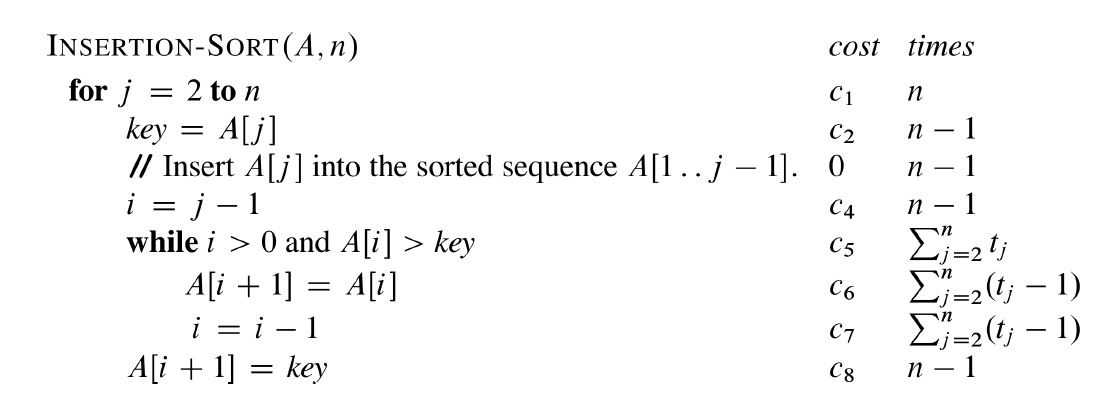
\includegraphics[width=0.9\linewidth]{insertion_sort.png}
    \end{figure}
    
    We are analyzing the time complexity of the \texttt{Insertion-Sort} algorithm. The cost of the algorithm is directly related to the number of times each step is repeated. Let’s go through the steps and calculate their costs.
    
    \subsection{Step-by-Step Cost Analysis}
    
    \begin{itemize}
        \item \textbf{Step 1:} The \texttt{for} loop iterates from $j = 2$ to $n$, so the condition is checked $n$ times, including the final check that fails. Hence, the total cost for this step is $c_1 \cdot n$.
        
        \item \textbf{Step 2:} The body of the \texttt{for} loop is executed $n-1$ times. Thus, this step has a cost of $c_2 \cdot (n-1)$.
        
        \item \textbf{Step 3:} The comment within the code is not executed, so its cost is $0$, even though it is "executed" $n-1$ times. Therefore, $c_3 = 0$.
        
        \item \textbf{Step 4:} The statement $i = j-1$ inside the \texttt{for} loop is executed $n-1$ times, hence the cost is $c_4 \cdot (n-1)$.
        
        \item \textbf{Step 5:} The \texttt{while} loop is nested inside the \texttt{for} loop. The cost depends on how many times the \texttt{while} loop is executed for each $j$, denoted as $t_j$. Therefore, the cost is the sum of $t_j$ from $j=2$ to $n$: 
        \[
        c_5 \cdot \sum_{j=2}^{n} t_j.
        \]
        
        \item \textbf{Steps 6 and 7:} The costs for these steps are also inside the \texttt{while} loop and depend on $t_j-1$, as the condition is not checked after the loop terminates. Hence, the total cost is:
        \[
        c_6 \cdot \sum_{j=2}^{n} (t_j - 1) + c_7 \cdot \sum_{j=2}^{n} (t_j - 1).
        \]
        
        \item \textbf{Step 8:} The assignment $A[i+1] = \texttt{key}$ occurs $n-1$ times, since it's inside the \texttt{for} loop. The total cost for this step is $c_8 \cdot (n-1)$.
    \end{itemize}
    
    \subsection{Overall Time Complexity}
    The total time complexity $T(n)$ of the \texttt{Insertion-Sort} algorithm is the sum of all these contributions:
    \[
    T(n) = c_1 \cdot n + c_2 \cdot (n-1) + 0 + c_4 \cdot (n-1) + c_5 \cdot \sum_{j=2}^{n} t_j + (c_6 + c_7) \cdot \sum_{j=2}^{n} (t_j - 1) + c_8 \cdot (n-1).
    \]
    
    \subsection{Best Case Scenario}
    In the best case, the input sequence is already sorted. This means that for all $j$, $t_j = 1$ (the \texttt{while} loop does not run). The time complexity becomes:
    \[
    T(n) = c_1 \cdot n + c_2 \cdot (n-1) + c_4 \cdot (n-1) + c_8 \cdot (n-1),
    \]
    which simplifies to:
    \[
    T(n) = (c_1 + c_2 + c_4 + c_8) \cdot n - (c_2 + c_4 + c_8).
    \]
    If we denote the constants as $b = c_1 + c_2 + c_4 + c_8$ and $d = -(c_2 + c_4 + c_8)$, the best case complexity is:
    \[
    T(n) = bn + d.
    \]
    In this case, everything inside the \texttt{while} loop is skipped and we assume all the constant equal to 1. Therefore, $T(n) = 5n - 4$.
    
    \subsection{Worst Case Scenario}
    In the worst case, the input sequence is sorted in reverse order. Here, $t_j = j$, which means the \texttt{while} loop executes $j$ times for $j=2,...,n$. The total cost for steps 5, 6, and 7 is:
    \[
    \sum_{j=2}^{n} t_j = \frac{n(n+1)}{2} - 1,
    \]
    and for steps 6 and 7:
    \[
    \sum_{j=2}^{n} (t_j - 1) = \frac{n(n-1)}{2}.
    \]
    Thus, the total time complexity in the worst case becomes:
    \[
    T(n) = c_1 \cdot n + c_2 \cdot (n-1) + c_4 \cdot (n-1) + c_5 \cdot \left(\frac{n(n+1)}{2} - 1\right) + (c_6 + c_7) \cdot \frac{n(n-1)}{2} + c_8 \cdot (n-1).
    \]
    This simplifies to:
    \[
    T(n) = \frac{3}{2}n^2 + \frac{7}{2}n - 4.
    \]
    
    \subsection{General Case}
    In general, the time complexity in the best case is $T(n) = bn + c$, where $b$ and $c$ are real constants, while in the worst case, it is $T(n) = an^2 + bn + c$, where $a$, $b$, and $c$ are real constants.

    \section{Selection Sort}
    Selection Sort is a simple comparison-based sorting algorithm that works by repeatedly selecting the smallest (or largest) element from an unsorted portion of the array and swapping it with the first unsorted element. 
    
    \subsection{Example}
    Consider the array \( A = [2, 5, 6, 4, 1, 3] \). The goal is to sort this array in ascending order using Selection Sort.
    
    \subsection{Steps of the Algorithm}
    \begin{itemize}
        \item Initial Setup: Start with the first element of the array as the current position \( j \) (initially \( j = 1 \)).
        \item Finding the Minimum: Compare the element at smallest with each subsequent element in the array:
        \begin{verbatim}
            For \( i = j + 1 \) to \( n \):
                If \( A[i] < A[smallest] \), update smallest to \( i \).
        \end{verbatim}
        \item Swap: After the inner loop completes, swap the elements at positions \( j \) and smallest.
        \item Repeat: Increment \( j \) and repeat the process until the entire array is sorted.
    \end{itemize}
    
    \subsection{Detailed Example Steps}
    \begin{itemize}
        \item Step 1: \begin{itemize}
            \item \( j = 1 \): \( A = [2, 5, 6, 4, 1, 3] \)
            \item Smallest is initially at index 1 (value 2).
            \item Compare with elements at indices 2 to 6.
            \item Smallest value found at index 5 (value 1).
            \item Swap \( A[1] \) with \( A[5] \):
            \item Result: \( A = [1, 5, 6, 4, 2, 3] \)
        \end{itemize}
        \item Step 2: \begin{itemize}
            \item \( j = 2 \): \( A = [1, 5, 6, 4, 2, 3] \)
            \item Smallest is at index 2 (value 5).
            \item Compare with elements at indices 3 to 6.
            \item Smallest value found at index 5 (value 2).
            \item Swap \( A[2] \) with \( A[5] \):
            \item Result: \( A = [1, 2, 6, 4, 5, 3] \)
        \end{itemize}
        \item Further Steps: Continue this process until \( j = n-1 \).
    \end{itemize}
    
    \subsection{Complexity Analysis}
    Selection Sort has a consistent time complexity of \( O(n^2) \), regardless of the initial order of the elements. This is because the algorithm always examines every element to find the minimum for each position in the array.
    
    There are no best-case or worst-case scenarios that can reduce the complexity since the algorithm must always perform the same number of comparisons.
    
    \subsection{Pseudocode}
    The pseudocode for Selection Sort is as follows:
    
    \begin{verbatim}
    n = length(A)
    for j = 1 to n - 1 do:
        smallest = j
        for i = j + 1 to n do:
            if A[i] < A[smallest] then
                smallest = i
        exchange A[j] with A[smallest]
    \end{verbatim}
    In Python, the exchange can be implemented using a temporary variable:
    \begin{verbatim}
    tmp = A[j]
    A[j] = A[smallest]
    A[smallest] = tmp
    \end{verbatim}
    
    \subsection{Cost Analysis}
    Let's denote the cost of each operation in the pseudocode:
    
    \begin{enumerate}
        \item Step 1 is executed once: \( 1 \)
        \item Step 2 is executed \( n \) times: \( n \)
        \item Step 3 is executed \( n-1 \) times: \( n - 1 \)
        \item Steps 4 and 5 are the sum of \( j \) from \( 1 \) to \( n-1 \): \( \sum_{j=1}^{n-1} t_j \)
        \item Steps 6 is the sum of \( j \) from \( 1 \) to \( n-1 \): \( 2 \sum_{j=1}^{n-1} (t_j - 1) \)
        \item Step 7 is executed \( n - 1 \) times: \( n - 1 \)
    \end{enumerate}
    The total cost \( T(n) \) in operations is given by:
    \[
    T(n) = 1 + n + (n - 1) + \sum_{j=1}^{n-1} t_j + 2 \sum_{j=1}^{n-1} (t_j - 1) + (n - 1)
    \]
    Using the steps for Insertion Sort, we can derive that:
    \[
    T(n) = 3n - 1 + \frac{n(n-1)}{2} + n(n-1) - 1
    \]
    Thus, the complexity of Selection Sort is in the order of \( O(n^2) \), it's remains the same for the best and worst case since we have to do the two for loops.
    
    \section{When to Use Selection Sort vs Insertion Sort}
    Selection Sort is generally not stable and does not perform well on large datasets due to its \( O(n^2) \) complexity. However, it has the advantage of performing a constant number of swaps, making it useful when memory writes are costly. \newline
    Insertion Sort, on the other hand, is more efficient for smaller datasets or partially sorted arrays, as it has a best-case time complexity of \( O(n) \) when the array is already sorted. Thus, Insertion Sort is preferable when dealing with nearly sorted data or small lists. In the best case Insertion sort is only $\Theta(n)$ since it doesn't enter the while loop.

\chapter{Divide and Conquer}

    \section{Recursive Algorithms}
    Before discussing divide-and-conquer algorithms, it is essential to understand the concept of recursive algorithms. A recursive algorithm is one that calls itself one or more times to solve a problem. The core idea is to divide the problem into smaller and simpler sub-problems, solve them individually, and then combine the solutions.
    
    A classical example is calculating the power of a number. For instance, calculating \(2^3\) can be done recursively by breaking it down as:
    \[
    2^3 = 2 \times 2^2 = 2 \times (2 \times 2^1)
    \]
    
    Recursion differs from iteration. While iteration involves loops, recursion involves a function calling itself. Iteration is generally more efficient in terms of constant factors, but recursion can simplify the design of an algorithm.
    
    \subsection{Base Case in Recursion}
    
    It is crucial that every recursive algorithm includes a base case, which provides a condition to stop the recursion. Without a base case, the algorithm would continue to call itself infinitely, leading to a stack overflow.
    
    \subsection{Execution Stack}
    Each time a recursive call is made, the current state of the function is saved in the execution stack (a LIFO structure). This is similar to a stack of objects where new items are added to the top. Once a function completes, its state is removed from the stack, and the previous function call is resumed. 
    
    For example, the execution stack for the function \texttt{RECURSIVE-POWER(2,3)} works as follows:
    
    \begin{itemize}
        \item The initial call \texttt{RECURSIVE-POWER(2,3)} leads to the call \texttt{RECURSIVE-POWER(2,2)}.
        \item Then, \texttt{RECURSIVE-POWER(2,2)} calls \texttt{RECURSIVE-POWER(2,1)}.
        \item Once \texttt{RECURSIVE-POWER(2,1)} returns the result, the previous calls are resumed until the final result is computed.
    \end{itemize}
    
    \section{Divide-and-Conquer Strategy}
    
    The divide-and-conquer strategy is commonly used in recursive algorithms. This strategy involves three main steps:
    \begin{itemize}
        \item \textbf{Divide:} Break the problem into smaller sub-problems.
        \item \textbf{Conquer:} Solve each sub-problem recursively.
        \item \textbf{Combine:} Combine the solutions of the sub-problems to form the final solution.
    \end{itemize}
    
    A classical example of this strategy is the \textbf{Merge-Sort} algorithm.
    
    \subsection{Merge-Sort Algorithm}
    
    Merge-sort is a sorting algorithm that follows the divide-and-conquer paradigm. Here are the steps:
    \begin{enumerate}
        \item Assume we have an unordered sequence of \(n\) elements.
        \item \textbf{Divide:} Split the sequence into two halves, each of length \(n/2\).
        \item \textbf{Conquer:} Sort both halves recursively using merge-sort.
        \item \textbf{Combine:} Merge the two sorted halves into one sorted sequence.
    \end{enumerate}
    
    The key part of the algorithm is the \textbf{combine} step, where two sorted arrays are merged.
    \begin{figure}[h!]
        \centering
        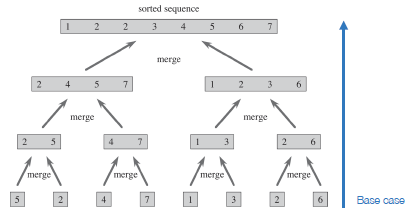
\includegraphics[width=0.75\linewidth]{immagini/merge_sort.png}
    \end{figure}
    \subsubsection{Merge-Sort Pseudo code}
    
    \begin{verbatim}
    MERGE-SORT(A, p, r)
        if p >= r
            return
        q = (p + r) / 2
        MERGE-SORT(A, p, q)
        MERGE-SORT(A, q+1, r)
        MERGE(A, p, q, r)
    \end{verbatim}
    
    Here, \(p\) and \(r\) represent the indices of the first and last elements of the array, and \(q\) is the middle index. The array is recursively split and sorted, and finally, the \texttt{MERGE} procedure combines the results.
    
    \subsubsection{Merge Procedure Pseudo code}
    
    \begin{verbatim}
    MERGE(A, p, q, r)
        n1 = q - p + 1
        n2 = r - q
        let L[1..n1+1] and R[1..n2+1] be new arrays
        for i = 1 to n1
            L[i] = A[p + i - 1]
        for j = 1 to n2
            R[j] = A[q + j]
        L[n1+1] = +infinite
        R[n2+1] = +infinite
        i = 1
        j = 1
        for k = p to r
            if L[i] <= R[j]
                A[k] = L[i]
                i = i + 1
            else
                A[k] = R[j]
                j = j + 1
    \end{verbatim}
    
    The \texttt{MERGE} function combines two sorted sub-arrays, \(L\) and \(R\), into a single sorted array. The use of sentinel values (\(\infty\)) ensures that the merging process can terminate correctly without additional checks.
    
    \section{Cost Analysis of Merge-Sort}
    The cost of Merge-Sort can be analyzed using recurrence relations. Here's the step-by-step breakdown:
    
    \subsection{Step 1: Divide the Array}
    
    Each time we divide the array, the size of the problem is halved. This results in two sub-problems of size \(n/2\). The time required to divide the array into two halves is constant, specifically \(\Theta(1)\), since it only involves calculating the midpoint \(q = (p + r) / 2\).
    
    \subsection{Step 2: Conquer the sub-problems}
    
    The two sub-problems are solved recursively, and the time to solve each sub-problem is given by the same merge-sort process. Therefore, the time required for solving both halves is \(T(n/2)\).
    
    \subsection{Step 3: Combine the Results (Merge Step)}
    
    The \texttt{MERGE} function takes \(\Theta(n)\) time because it processes all elements of the two sub-arrays, comparing and merging them into a single array. The merging process requires one pass through the elements, resulting in linear time complexity.
    
    \subsection{Overall Recurrence Relation}
    
    The time complexity of merge-sort can be described by the following recurrence relation:
    \[
    T(n) = 2T\left(\frac{n}{2}\right) + \Theta(n)
    \]
    This relation reflects the fact that we are solving two sub-problems of size \(n/2\), and the merging step takes \(\Theta(n)\) time.
    
    \subsection{Solving the Recurrence Relation}
    
    To solve this recurrence relation, we can use the \textbf{recursion tree method} or the \textbf{master theorem}. Let's go through the steps:
    \begin{enumerate}
        \item Recursive Expansion: Start by expanding the recurrence relation:
       \[
       T(n) = 2T\left(\frac{n}{2}\right) + \Theta(n)
       \]
       \[
       = 2\left(2T\left(\frac{n}{4}\right) + \Theta\left(\frac{n}{2}\right)\right) + \Theta(n)
       \]
       \[
       = 4T\left(\frac{n}{4}\right) + 2\Theta\left(\frac{n}{2}\right) + \Theta(n)
       \]
       \[
       = 8T\left(\frac{n}{8}\right) + 4\Theta\left(\frac{n}{4}\right) + 2\Theta\left(\frac{n}{2}\right) + \Theta(n)
       \]
       After expanding \(k\) times, we obtain:
       \[
       T(n) = 2^k T\left(\frac{n}{2^k}\right) + \sum_{i=0}^{k-1} 2^i \Theta\left(\frac{n}{2^i}\right)
       \] 
        \item Base Case:
       The base case occurs when the size of the sub-problem becomes 1, i.e., when \(n/2^k = 1\), which implies \(k = \log_2 n\). Substituting this into the expansion:
       \[
       T(n) = 2^{\log_2 n} T(1) + \sum_{i=0}^{\log_2 n - 1} 2^i \Theta\left(\frac{n}{2^i}\right)
       \]
       Since \(T(1)\) is a constant, we get:
       \[
       T(n) = n \cdot \Theta(1) + \sum_{i=0}^{\log_2 n - 1} \Theta(n)
       \]
        \item Sum Simplification:
       The sum simplifies to:
       \[
       \sum_{i=0}^{\log_2 n - 1} \Theta(n) = \log_2 n \cdot \Theta(n)
       \]
        \item Final Time Complexity:
       Therefore, the total time complexity is:
       \[
       T(n) = \Theta(n) + \log_2 n \cdot \Theta(n) = \Theta(n \log n)
       \]
    \end{enumerate}
        
    \subsection{Summary of Merge-Sort Complexity}
    
    Merge-Sort has a time complexity of \(\Theta(n \log n)\), which is optimal for comparison-based sorting algorithms. This time complexity holds for both the average and worst cases due to the divide-and-conquer structure, where the number of levels in the recursion tree is \(\log_2 n\), and each level performs \(\Theta(n)\) work for merging. The height of the tree is $h = log_2 n + 1$ and it has $n$ leaves.

\section{Recursion Tree Method for Complexity Analysis}

The recursion tree method is a visual tool to help analyze the complexity of recursive functions. Let’s consider the following exercises to explore this method in detail.

\subsection{Exercise 1: Analyzing \( T(n) = 3T\left(\frac{n}{4}\right) + \Theta(n^2) \)}
Given the recurrence relation:
\[
T(n) = 3T\left(\frac{n}{4}\right) + c n^2
\]
where \(c > 0\), \(a = 3\) is the number of subproblems, and \(b = 4\) represents the factor by which the problem size is reduced. The initial cost function \(cn^2\) is quadratic, meaning that the cost at each level will follow this quadratic pattern as the problem size decreases.

\subsection{Step-by-Step Analysis Using Recursion Tree}
\begin{enumerate}
    \item \textbf{Root Level}: At the root, the cost is \(cn^2\).

    \item \textbf{First Level of Subproblems}: We divide the problem into three subproblems, each of size \(n/4\), with cost:
   \[
   3 \cdot \left(\frac{n}{4}\right)^2 \cdot c = \frac{3}{16} n^2 c
   \]

    \item \textbf{Second Level}: Each subproblem of size \(n/4\) is divided again, resulting in three more subproblems per branch. The cost at this level becomes:
   \[
   \left(\frac{3}{16}\right)^2 n^2 c
   \]

    \item \textbf{Recursive Pattern}: We continue this process until reaching the leaves of the recursion tree, where the cost is constant (\(T(1)\)).
\end{enumerate}


\subsection{Calculating Total Cost}

The height of the tree is:
\[
h = \log_b n = \log_4 n
\]
and the number of leaves at the final level is approximately \(n\).

The total cost \(T(n)\) is the sum of the costs across each level:
\[
T(n) = \sum_{i=0}^{\log_4 n - 1} \left(\frac{3}{16}\right)^i \cdot c \, n^2 + \Theta(n^{\log_4 3})
\]

We can approximate this sum with an infinite geometric series:
\[
T(n) < \sum_{i=0}^{\infty} \left(\frac{3}{16}\right)^i \cdot c \, n^2
\]

Using the formula for the sum of an infinite geometric series \(\sum_{k=0}^{\infty} x^k = \frac{1}{1-x}\) for \(|x| < 1\), we get:
\[
T(n) < \frac{1}{1 - \frac{3}{16}} \cdot c \, n^2 + \Theta(n^{\log_4 3}) = \frac{16}{13} c \, n^2 + \Theta(n^{\log_4 3})
\]
Thus, we conclude:
\[
T(n) = O(n^2)
\]

\begin{center}
    \textbf{Recursion Tree for \(T(n) = 3T\left(\frac{n}{4}\right) + \Theta(n^2)\)}
\end{center}

\begin{tikzpicture}
    [level distance=1.5cm, sibling distance=4cm, edge from parent/.style={draw,-latex}]
    \node { \( T(n) = cn^2 \) }
        child { node { \( T(n/4) = \frac{3}{16} cn^2 \) }
            child { node { \( T(n/16) = \left(\frac{3}{16}\right)^2 cn^2 \) } }
            child { node { \( T(n/16) = \left(\frac{3}{16}\right)^2 cn^2 \) } }
            child { node { \( T(n/16) = \left(\frac{3}{16}\right)^2 cn^2 \) } }
        }
        child { node { \( T(n/4) = \frac{3}{16} cn^2 \) } }
        child { node { \( T(n/4) = \frac{3}{16} cn^2 \) } };
\end{tikzpicture}

\subsection{Exercise 2: Analyzing \( T(n) = T\left(\frac{n}{3}\right) + T\left(\frac{2n}{3}\right) + cn \)}

Given the recurrence relation:
\[
T(n) = T\left(\frac{n}{3}\right) + T\left(\frac{2n}{3}\right) + cn
\]
\begin{enumerate}
    \item Root Level: At the root, the cost is \(cn\).
    \item Division into Subproblems: We divide the problem into subproblems of size \(n/3\) and \(2n/3\), each with cost proportional to \(cn\). 
    \item Continuing the Division: This is an unbalanced tree, as the \(2n/3\) branch will continue dividing for more levels than the \(n/3\) branch.
\end{enumerate}

Since the right branch (\(2n/3\)) divides more slowly, it will dominate the total cost. Therefore, we approximate the cost by following the longer branch.

\subsection{Calculating Height and Total Cost}

The height \(h\) of the tree based on the \(2n/3\) branch is:
\[
h = \log_{3/2} n
\]
Since each level has a cost \(cn\), the total cost is:
\[
T(n) = cn \cdot \log_{3/2} n = O(n \log n)
\]

\begin{center}
    \textbf{Partial Recursion Tree for \(T(n) = T\left(\frac{n}{3}\right) + T\left(\frac{2n}{3}\right) + cn\)}


\begin{tikzpicture}
    [level distance=1.5cm, sibling distance=3cm, edge from parent/.style={draw,-latex}]
    \node { \( T(n) = cn \) }
        child { node { \( T(n/3) = \frac{1}{3} cn \) } }
        child { node { \( T(2n/3) = \frac{2}{3} cn \) }
            child { node { \( T(2n/9) = \frac{2}{9} cn \) }
                child { node { \(\cdots\) } }
            }
            child { node { \( T(4n/9) = \frac{4}{9} cn \) }
                child { node { \(\cdots\) } }
            }
        };
\end{tikzpicture}
\end{center}
\subsection{Summary}

In general, for a recurrence relation \( T(n) = a T\left(\frac{n}{b}\right) + \Theta(n^\alpha) \):
\begin{itemize}
    \item The recursion tree height is \( h = \log_b n \).
    \item The cost at each level is determined by the number of subproblems \(a\), the size reduction factor \(b\), and the initial complexity \(\alpha\).
    \item The total cost is derived from the sum of work at each level, up to the leaves.
\end{itemize}

\section{Exercise: Algorithm with Complexity \(\Theta(n \log n)\)}

Given a set \(S\) of \(n\) integers and another integer \(X\), determine if there exists a pair of elements in \(S\) whose sum equals \(X\). Note that we only need to find one such pair if it exists; it does not matter which pair.

A straightforward brute-force approach would involve two nested loops: for each element \(y \in S\), check if there exists another element \(w \in S\) such that \(y + w = X\). However, this approach has a time complexity of \(\Theta(n^2)\), which is suboptimal.

\subsection{Optimized Approach}
We aim to achieve a time complexity of \(\Theta(n \log n)\). Since sorting algorithms like merge-sort have this complexity, we can leverage sorting in our solution.

If there exist elements \(y, w \in S\) such that \(y + w = X\), then:
\[
w = X - y
\]
Define a new set \(S'\) as follows:
\[
            S' = \{z = X - y \mid y \in S\}
            \]
\begin{itemize}
    \item Sort \(S\) and \(S'\) using merge-sort, each with a time complexity of \(\Theta(n \log n)\).
    \item Merge \(S\) and \(S'\) into a new sequence \(S''\).
    \item Check if there exists an element in \(S\) that appears in \(S''\).
\end{itemize}

\subsection{Complexity Analysis}
\begin{itemize}
    \item Creating \(S'\) has a linear cost: \(\Theta(n)\).
    \item Sorting \(S\) and \(S'\) requires \(\Theta(n \log n)\).
    \item Merging \(S\) and \(S'\) takes linear time: \(\Theta(n)\).
    \item Checking for duplicate elements in \(S''\) also has a linear cost: \(\Theta(n)\).
\end{itemize}

Therefore, the total time complexity is:
\[
\Theta(n) + 2 \Theta(n \log n) = \Theta(n \log n)
\]

\section{Exercise: Finding an Element in a Sequence}

Given a sequence \(S\) of integers and an integer \(X\), determine whether \(X \in S\) and return the index \(i\) such that \(S[i] = X\).

\subsection{Linear Search}
If \(S\) is unordered, we must scan the entire sequence, resulting in a time complexity of \(\Theta(n)\). This is known as the linear scan.

\subsection{Binary Search}
If \(S\) is ordered, we can use binary search, which divides the search interval in half each step:
\begin{enumerate}
    \item Define two indices, \( \text{low} \) and \( \text{high} \).
    \item  Compute the midpoint as:
   \[
   \text{mid} = \left\lfloor \frac{\text{high} + \text{low}}{2} \right\rfloor
   \]
    \item If \(X < S[\text{mid}]\), continue searching in the left half \([ \text{low}, \text{mid} - 1 ]\).
    \item If \(X > S[\text{mid}]\), search in the right half \([ \text{mid} + 1, \text{high} ]\).
    \item If \(X = S[\text{mid}]\), return \(\text{mid}\).
\end{enumerate}
Each division reduces the search space by half, leading to a logarithmic time complexity: \(\Theta(\log n)\), which matches the height of a binary tree.

\subsection{Iterative Binary Search Algorithm}

\begin{verbatim}
def iterative_binary_search(S, X, low, high):
    while low <= high:
        mid = (high + low) // 2  # Equivalent to the floor of (high + low) / 2
        if S[mid] == X:
            return mid
        elif S[mid] < X:
            low = mid + 1
        else:
            high = mid - 1
    return None  # Return None if X is not found
\end{verbatim}

The \texttt{None} return indicates that the element was not found.

\subsection{Complexity Analysis}
The recurrence relation for the binary search is:
\[
T(n) = T\left(\frac{n}{2}\right) + \Theta(1)
\]
since each iteration reduces the problem size by half with a constant operation. Solving this recurrence, we find:
\[
T(n) = \Theta(\log n)
\]

\newpage

\chapter{Strassen Matrix Multiplication}
    
    Before introducing Strassen's method, let's examine standard matrix multiplication, called \textbf{Square-Matrix-Multiplication (SMMR)}. Given two \(n \times n\) matrices \(A\) and \(B\), we want to compute their product \(C = A \times B\).
    
    \subsection{Standard Matrix Multiplication (SMMR)}
    1. Divide matrices \(A\) and \(B\) as follows:
       \[
       A = \begin{bmatrix} A_{11} & A_{12} \\ A_{21} & A_{22} \end{bmatrix}, \quad B = \begin{bmatrix} B_{11} & B_{12} \\ B_{21} & B_{22} \end{bmatrix}
       \]
       
    2. Each element of \(C\) is computed as:
       \[
       C = A \times B = \begin{bmatrix} C_{11} & C_{12} \\ C_{21} & C_{22} \end{bmatrix}
       \]
       where
       \[
       C_{11} = A_{11} B_{11} + A_{12} B_{21}, \quad C_{12} = A_{11} B_{12} + A_{12} B_{22}
       \]
       \[
       C_{21} = A_{21} B_{11} + A_{22} B_{21}, \quad C_{22} = A_{21} B_{12} + A_{22} B_{22}
       \]
    
    This method requires 8 recursive multiplications for each submatrix.
    
    \subsection{Recursive SMMR Algorithm}
    
    \begin{verbatim}
    def SMMR(A, B):
        n = len(A)  # Number of rows in A
        C = [[0] * n for _ in range(n)]  # Initialize nxn matrix C with zeros
        
        if n == 1:
            C[0][0] = A[0][0] * B[0][0]
        else:
            # Partition matrices A, B, and C as described
            C11 = SMMR(A11, B11) + SMMR(A12, B21)
            C12 = SMMR(A11, B12) + SMMR(A12, B22)
            C21 = SMMR(A21, B11) + SMMR(A22, B21)
            C22 = SMMR(A21, B12) + SMMR(A22, B22)
            
            # Combine results into matrix C (requires additional merging steps in practice)
        
        return C
    \end{verbatim}
    
    \subsection{Complexity Analysis of SMMR}
    
    Dividing each matrix into four \( \frac{n}{2} \times \frac{n}{2} \) submatrices requires 8 multiplications. Assuming each submatrix has \( \left(\frac{n}{2}\right)^2 = \frac{n^2}{4} \) entries, we derive the recurrence:
    \[
    T(n) = \begin{cases} 
          \Theta(1) & \text{if } n = 1 \\
          8T\left(\frac{n}{2}\right) + \Theta(n^2) & \text{if } n > 1 
       \end{cases}
    \]
    
    The height of the recursion tree is \(\log_2 n\), and the total number of leaves is \(n^{\log_2 8} = n^3\), leading to:
    
    
    \section{Strassen's Algorithm}
    
    Strassen's algorithm presents a clever approach to improve the efficiency of matrix multiplication, specifically for large matrices. Although it is challenging to apply this algorithm beyond the context of matrix multiplication, studying it is highly useful for understanding the principles of recursion and complexity analysis in algorithms. 
    
    \subsection{Standard Recursive Matrix Multiplication}
    As previously discussed, multiplying two matrices \(A\) and \(B\) can be formulated as a recursive problem. Each matrix is divided into four \( \frac{n}{2} \times \frac{n}{2} \) submatrices, and recursive calls are made until we reach matrices of size \(1 \times 1\), where the multiplications are performed directly. This standard approach yields a time complexity of \(\Theta(n^3)\).
    
    \subsection{Overview of Strassen's Algorithm}
    Strassen’s algorithm reduces the complexity of matrix multiplication by leveraging specific combinations of additions and multiplications. It consists of four main steps:
    \begin{enumerate}
        \item Divide matrices \(A\) and \(B\) into \( \frac{n}{2} \times \frac{n}{2} \) submatrices, similar to the standard approach.
        \item Construct 10 intermediate matrices \( S_1, S_2, \dots, S_{10} \) of size \( \frac{n}{2} \times \frac{n}{2} \), each representing specific sums or differences of the submatrices of \(A\) and \(B\). These combinations are carefully chosen to optimize the calculation process, as we will see shortly. This step has a complexity of \(\Theta(n^2)\).
        \item Using the submatrices from steps 1 and 2, compute 7 product matrices \( P_1, P_2, \dots, P_7 \), each of size \( \frac{n}{2} \times \frac{n}{2} \), by recursively applying the Strassen algorithm.
        \item Finally, construct the resulting submatrices \( C_{11}, C_{12}, C_{21}, C_{22} \) for the product matrix \(C\), using the product matrices \(P_i\). This step also has a complexity of \(\Theta(n^2)\).
    \end{enumerate}
    
    The key improvement in Strassen's algorithm lies in reducing the number of recursive multiplications from 8 to 7, which reduces the overall complexity.
    
    \subsection{Detailed Steps of Strassen’s Algorithm}
    \subsubsection*{Step 1: Divide Matrices}
    This step involves partitioning \(A\) and \(B\) as:
    \[
    A = \begin{bmatrix} A_{11} & A_{12} \\ A_{21} & A_{22} \end{bmatrix}, \quad B = \begin{bmatrix} B_{11} & B_{12} \\ B_{21} & B_{22} \end{bmatrix}
    \]
    
    \subsubsection*{Step 2: Construct Intermediate Sum Matrices}
    Define the following intermediate matrices:
    \[
    \begin{aligned}
        S_1 &= B_{12} - B_{22}, \\
        S_2 &= A_{11} + A_{12}, \\
        S_3 &= A_{21} + A_{22}, \\
        S_4 &= B_{21} - B_{11}, \\
        S_5 &= A_{11} + A_{22}, \\
        S_6 &= B_{11} + B_{22}, \\
        S_7 &= A_{12} - A_{22}, \\
        S_8 &= B_{21} + B_{22}, \\
        S_9 &= A_{11} - A_{21}, \\
        S_{10} &= B_{11} + B_{12}.
    \end{aligned}
    \]
    
    \subsubsection*{Step 3: Compute Product Matrices}
    Calculate the seven product matrices as follows:
    \[
    \begin{aligned}
        P_1 &= A_{11} \cdot S_1, \\
        P_2 &= S_2 \cdot B_{22}, \\
        P_3 &= S_3 \cdot B_{11}, \\
        P_4 &= A_{22} \cdot S_4, \\
        P_5 &= S_5 \cdot S_6, \\
        P_6 &= S_7 \cdot S_8, \\
        P_7 &= S_9 \cdot S_{10}.
    \end{aligned}
    \]
    
    \subsubsection*{Step 4: Construct Final Product Matrix \(C\)}
    Using the product matrices \(P_1, P_2, \dots, P_7\), construct the final submatrices of \(C\):
    \[
    \begin{aligned}
        C_{11} &= P_5 + P_4 - P_2 + P_6, \\
        C_{12} &= P_1 + P_2, \\
        C_{21} &= P_3 + P_4, \\
        C_{22} &= P_5 + P_1 - P_3 - P_7.
    \end{aligned}
    \]
    The final product matrix \(C\) is given by:
    \[
    C = \begin{bmatrix} C_{11} & C_{12} \\ C_{21} & C_{22} \end{bmatrix}
    \]
    
    \subsection{Complexity Analysis of Strassen's Algorithm}
    Despite the algorithm's complexity in terms of individual operations, it reduces the number of multiplications needed, which decreases the overall complexity. Strassen's algorithm achieves a time complexity of:
    \[
    \Theta(n^{\log_2 7}) \approx \Theta(n^{2.8073})
    \]
    This represents a significant improvement over the standard matrix multiplication complexity of \(\Theta(n^3)\).

\chapter{The Master Theorem for Solving Recurrences}

\section{Introduction}

The \textbf{Master Theorem} provides a systematic way to analyze divide-and-conquer recurrences of the form:  
\[
T(n) = aT\left(\frac{n}{b}\right) + f(n)
\]
where:
\begin{itemize}
    \item \(a \geq 1\): Number of subproblems.
    \item \(b > 1\): Factor by which the input size is divided in each recursive step.
    \item \(f(n)\): Cost outside the recursive calls, often referred to as the "work" term.
\end{itemize}
The theorem helps determine the asymptotic complexity of \(T(n)\) without solving the recurrence fully. The theorem can not be applied if:
\begin{itemize}
    \item T(n) is not monotone, for example T(n) = sinx
    \item f(n) is not polynomial, for example f(n) = $2^x$
    \item b cannot be expressed as a constant, for example T(n) = T($\sqrt{n}$)
\end{itemize}

\section{Cases of the Master Theorem}

Let \(c = \log_b a\), representing the growth rate of the recursive tree. The complexity of \(T(n)\) depends on the relationship between \(f(n)\) and \(n^c\):

\subsection{Case 1: \(f(n) = O(n^{c - \epsilon})\)}
If \(f(n)\) grows slower than \(n^c\) by a polynomial factor (\(\epsilon > 0\)), then:  
\[
T(n) = \Theta(n^c)
\]

\subsection{Case 2: \(f(n) = \Theta(n^c)\)}
If \(f(n)\) and \(n^c\) grow at the same rate, then:  
\[
T(n) = \Theta(n^c \log n)
\]
The general formula is that if f(n) = $\theta(n^c log^kn)$ and \(f(n)\) and \(n^c\) grow at the same rate, then:
\[
T(n) = \Theta(n^c \log^{k+1}n)
\]

\subsection{Case 3: \(f(n) = \Omega(n^{c + \epsilon})\)}
If \(f(n)\) grows faster than \(n^c\) by a polynomial factor (\(\epsilon > 0\)) and the \textit{regularity condition} \(a f(\frac{n}{b}) \leq cf(n)\) (for \(c < 1\) and n sufficiently large) holds, then:  
\[
T(n) = \Theta(f(n))
\]

\subsection{Key notes:}
This theorem says that we choose the larger function comparing our $f(n)$ with $n^{\log_b a}$. The first case says $n^{\log_b a}$ is larger than $f(n)$ because we can equalize $f(n)$ to $n^{\log_b a}$ by subtracting a possible epsilon greater than zero. If we can do it then we have the first case. The last case says that $f(n)$ is larger than $n^{\log_b a}$ then $T(n) = \Theta(f(n))$. The second case says that the two functions are the same  $\rightarrow T(n) = \Theta(n^{\log_b a}\log n)$. If we are between cases we can not use the master theorem, if we are lucky we will know the answer immediately with the master theorem.


\section{Examples}

\subsection{Strassen's Algorithm}
\[
T(n) = 7T\left(\frac{n}{2}\right) + \Theta(n^2)
\]
\begin{itemize}
    \item \(a = 7\), \(b = 2\), \(f(n) = n^2\).
    \item \(c = \log_2 7 \approx 2.807\).
    \item Compare \(f(n) = n^2\) to \(n^{\log_2 7}\): \(f(n) = O(n^{c - \epsilon})\), \(\epsilon = 0.807\).
\end{itemize}
By Case 1:  
\[
T(n) = \Theta(n^{\log_2 7})
\]

\subsection{Example: \(T(n) = 9T(n/3) + n\)}
\begin{itemize}
    \item \(a = 9\), \(b = 3\), \(f(n) = n\).
    \item \(c = \log_3 9 = 2\).
    \item \(f(n) = O(n^{c - 1})\).
\end{itemize}
By Case 1:  
\[
T(n) = \Theta(n^2)
\]

\subsection{Example: \(T(n) = T(2n/3) + 1\)}
\begin{itemize}
    \item \(a = 1\), \(b = 3/2\), \(f(n) = 1\).
    \item \(c = \log_{3/2} 1 = 0\).
    \item \(f(n) = \Theta(1)\).
\end{itemize}
By Case 2:  
\[
T(n) = \Theta(\log n)
\]
We look if $n^{\log_{\frac{3}{2}} 1} = n^0 = 1$, since they are equal we are in case 2, therefore $T(n) = \Theta(n^{\log_b a} \log n) = \Theta(n^{\log_{\frac{3}{2}} 1} \log n) = \Theta(\log n)$ since the $n^x$ term is equal to one!

\subsection{Exercise: \(T(n) = 3T(n/4) + n \log n\)}

\begin{itemize}
    \item Parameters:
    \begin{itemize}
        \item \(a = 3\), \(b = 4\), \(f(n) = n \log n\).
        \item \(n^{\log_b a} = n^{\log_4 3} = n^{0.792}\).
    \end{itemize}
    \item Analysis:
    \begin{itemize}
        \item \(f(n) = \Omega(n^{\log_4 3 + \epsilon})\), with \(\epsilon \approx 0.2\).
        \item Check the regularity condition:
        \[
        af\left(\frac{n}{b}\right) = 3 \left(\frac{n}{4}\right) \log\left(\frac{n}{4}\right) \leq \frac{3}{4}n \log(n) = cf(n), \quad c = \frac{3}{4}.
        \]
        \item Regularity condition holds as \(c < 1\).
    \end{itemize}
    \item Conclusion: By the third case of the Master Theorem:
    \[
    T(n) = \Theta(n \log n).
    \]
\end{itemize}

\subsection{Exercise: \(T(n) = 2T(n/2) + n \log n\)}

\begin{itemize}
    \item Parameters:
    \begin{itemize}
        \item \(a = 2\), \(b = 2\), \(f(n) = n \log n\).
        \item \(n^{\log_b a} = n^{\log_2 2} = n\).
    \end{itemize}
    \item Analysis:
    \begin{itemize}
        \item Compare \(f(n)\) and \(n^{\log_b a}\):
        \[
        \frac{f(n)}{n^{\log_b a}} = \frac{n \log n}{n} = \log n.
        \]
        \item \(\log n < n^\epsilon\) asymptotically, but \(f(n)\) is not polynomially larger than \(n^{\log_b a}\).
    \end{itemize}
    \item Conclusion: The Master Theorem cannot be applied since \(f(n)\) is between the second and third case.
\end{itemize}

\subsection{Exercise 3: \(T(n) = 2T(n/2) + \frac{n}{\log n}\)}

\begin{itemize}
    \item Parameters:
    \begin{itemize}
        \item \(a = 2\), \(b = 2\), \(f(n) = \frac{n}{\log n}\).
        \item \(n^{\log_b a} = n^{\log_2 2} = n\).
    \end{itemize}
    \item Analysis:
    \begin{itemize}
        \item Compare \(f(n)\) and \(n^{\log_b a}\):
        \[
        \frac{f(n)}{g(n)} = \frac{\frac{n}{\log n}}{n} = \frac{1}{\log n}.
        \]
        \item As \(n \to \infty\), \(\frac{1}{\log n} \to 0\), so \(f(n) = O(n)\).
        \item Check if \(f(n) = O(n^{\log_b a - \epsilon})\):
        \[
        \lim_{n \to \infty} \frac{\frac{n}{\log n}}{n^{1-\epsilon}} = \frac{n^\epsilon}{\log n} \to \infty, \quad \text{(using L'Hôpital's Rule)}.
        \]
        \item Therefore, \(f(n)\) is not polynomially smaller than \(n\), and we are between cases.
    \end{itemize}
    \item Conclusion: The Master Theorem cannot be applied since \(f(n)\) is between cases 1 and 2.
\end{itemize}





\section{Exercises}

\subsection{Exercise 1: \(T(n) = 8T(n/2) + 1000n^2\)}

\begin{itemize}
    \item Parameters:
    \begin{itemize}
        \item \(a = 8\), \(b = 2\), \(f(n) = 1000n^2\).
        \item \(n^{\log_b a} = n^{\log_2 8} = n^3\).
    \end{itemize}
    \item Analysis:
    \begin{itemize}
        \item Check if \(f(n) = O(n^{3-\epsilon})\):
        \[
        c n^2 = O(n^{3-\epsilon}) \quad \text{for any } 0 < \epsilon < 1.
        \]
        \item Since \(f(n)\) satisfies the condition, we conclude \(T(n) = \Theta(n^3)\).
        \item Verify if \(f(n)\) is polynomially smaller:
        \[
        \lim_{n \to \infty} \frac{c n^2}{n^{3-\epsilon}} = \frac{\infty}{\infty}.
        \]
        Using L'Hôpital's Rule:
        \[
        \lim_{n \to \infty} \frac{2c n}{(3-\epsilon)n^{2-\epsilon}} = 0.
        \]
        Thus, \(f(n)\) is polynomially smaller.
    \end{itemize}
    \item Conclusion:
    \[
    T(n) = \Theta(n^3).
    \]
\end{itemize}

\subsection{Exercise 2: \(T(n) = 2T(n/2) + 10n\)}

\begin{itemize}
    \item Parameters:
    \begin{itemize}
        \item \(a = 2\), \(b = 2\), \(f(n) = \Theta(n)\).
        \item \(n^{\log_b a} = n^{\log_2 2} = n\).
    \end{itemize}
    \item Analysis:
    \begin{itemize}
        \item Since \(f(n) = \Theta(n)\), it satisfies the second case of the Master Theorem.
    \end{itemize}
    \item Conclusion:
    \[
    T(n) = \Theta(n \log n).
    \]
\end{itemize}

\subsection{Exercise 3: \(T(n) = 2T(n/2) + 10n^2\)}

\begin{itemize}
    \item Parameters:
    \begin{itemize}
        \item \(a = 2\), \(b = 2\), \(f(n) = 10n^2\).
        \item \(n^{\log_b a} = n^{\log_2 2} = n\).
    \end{itemize}
    \item Analysis:
    \begin{itemize}
        \item Check if \(f(n) = \Omega(n^{1+\epsilon})\): Yes.
        \item Verify the regularity condition:
        \[
        2 \cdot \frac{n^2}{2} < c \cdot 10n^2, \quad c < 1.
        \]
        The condition is satisfied. Because it results that $c > \frac{1}{2}$.
    \end{itemize}
    \item Conclusion:
    \[
    T(n) = \Theta(f(n)) = \Theta(n^2).
    \]
\end{itemize}

\subsection{Exercise 4: \(T(n) = 4T(n/2) + \frac{n^2}{\log n}\)}

\begin{itemize}
    \item Parameters:
    \begin{itemize}
        \item \(a = 4\), \(b = 2\), \(f(n) = \frac{n^2}{\log n}\).
        \item \(n^{\log_b a} = n^{\log_2 4} = n^2\).
    \end{itemize}
    \item Analysis:
    \begin{itemize}
        \item Check if \(f(n) = O(n^{2-\epsilon})\):
        \[
        \lim_{n \to \infty} \frac{\frac{n^2}{\log n}}{n^2} = \frac{1}{\log n} \to 0.
        \]
        \(f(n)\) grows slower than \(n^2\).
        \item Check if \(f(n)\) is polynomially smaller:
        \[
        \lim_{n \to \infty} \frac{\frac{n^2}{\log n}}{n^{2-\epsilon}} = \frac{n^\epsilon}{\log n} = \frac{\infty}{\infty}.
        \]
        Using L'Hôpital's Rule:
        \[
        \lim_{n \to \infty} \frac{\epsilon n^{\epsilon - 1}}{\frac{1}{n}} = \infty.
        \]
        \(f(n)\) is not polynomially smaller.
    \end{itemize}
    \item Conclusion:
    \[
    \text{The Master Theorem cannot be applied, as \(f(n)\) is between cases 1 and 2.}
    \]
\end{itemize}

\section{Proof of the Master Theorem}

\subsection{Theorem for Exact Powers of \(b > 1\)}

We start by proving the theorem for exact powers of \(b > 1\) such that \(n = 1, b, b^2, \ldots\).

\[
T(n) = aT\left(\frac{n}{b}\right) + f(n)
\]

This proof is structured around three lemmas:

\begin{enumerate}
    \item \textbf{Lemma 1:} Reduces the recurrence to an equation involving a summation.
    \item \textbf{Lemma 2:} Provides asymptotic bounds for this summation.
    \item \textbf{Lemma 3:} Combines the results of the first two lemmas to prove the Master Theorem.
\end{enumerate}

\subsection{Lemma 1}

Let \(a \geq 1\) and \(b > 1\) be constants, and let \(f(n)\) be a non-negative function defined on exact powers of \(b\). Define \(T(n)\) by the recurrence:

\[
T(n) =
\begin{cases} 
\Theta(1) & \text{if } n = 1, \\
aT\left(\frac{n}{b}\right) + f(n) & \text{if } n = b^i, i \in \mathbb{N}.
\end{cases}
\]

Then, 

\[
T(n) = \Theta\left(n^{\log_b a}\right) + \sum_{j=0}^{\log_b n - 1} a^j f\left(\frac{n}{b^i}\right).
\]

\paragraph{Proof of Lemma 1:}
We construct a recursion tree to analyze the recurrence.

\begin{forest}
    for tree={
        grow'=south, 
        circle, 
        draw, 
        minimum size=1.2em, 
        inner sep=1pt, 
        s sep+=10pt, 
        l sep+=10pt
    }
    [
        \(f(n)\) 
        [\(a f\left(\frac{n}{b}\right)\)
            [\(a^2 f\left(\frac{n}{b^2}\right)\)
                [\(\cdots\)
                    [\(\Theta(1)\)]
                ]
                [\(\cdots\)
                    [\(\Theta(1)\)]
                ]
            ]
            [\(a^2 f\left(\frac{n}{b^2}\right)\)
                [\(\cdots\)
                    [\(\Theta(1)\)]
                ]
                [\(\cdots\)
                    [\(\Theta(1)\)]
                ]
            ]
        ]
        [\(a f\left(\frac{n}{b}\right)\)
            [\(a^2 f\left(\frac{n}{b^2}\right)\)
                [\(\cdots\)
                    [\(\Theta(1)\)]
                ]
                [\(\cdots\)
                    [\(\Theta(1)\)]
                ]
            ]
            [\(a^2 f\left(\frac{n}{b^2}\right)\)
                [\(\cdots\)
                    [\(\Theta(1)\)]
                ]
                [\(\cdots\)
                    [\(\Theta(1)\)]
                ]
            ]
        ]
        [\(a f\left(\frac{n}{b}\right)\)
            [\(a^2 f\left(\frac{n}{b^2}\right)\)
                [\(\cdots\)
                    [\(\Theta(1)\)]
                ]
                [\(\cdots\)
                    [\(\Theta(1)\)]
                ]
            ]
            [\(a^2 f\left(\frac{n}{b^2}\right)\)
                [\(\cdots\)
                    [\(\Theta(1)\)]
                ]
                [\(\cdots\)
                    [\(\Theta(1)\)]
                ]
            ]
        ]
    ]
\end{forest}


The cost of this algorithm is given by:
\begin{itemize}
    \item The root contributes \(f(n)\).
    \item The second level contributes \(a f(n/b)\).
    \item The third level contributes \(a^2 f(n/b^2)\).
    \item The \(i\)-th level contributes \(a^i f(n/b^i)\).
    \item The leaves contribute \(\Theta\left(n^{\log_b a}\right)\).
\end{itemize}
Summing the contributions from all levels:

\[
T(n) = \sum_{j=0}^{\log_b a - 1} a^j f\left(\frac{n}{b^j}\right) + \Theta\left(n^{\log_b a}\right).
\]

The terms represent the cost of the internal levels and the cost of the leaves, respectively. The Master Theorem distinguishes between cases where:
\begin{itemize}
    \item The cost of the leaves dominates.
    \item The cost of the root dominates.
    \item The costs are balanced.
\end{itemize}

\subsection{Lemma 2}

Let \(a > 1\), \(b > 1\), and \(f(n)\) be a non-negative function defined on exact powers of \(b\). Define the star function \(g(n)\) as:

\[
g(n) = \sum_{j=0}^{\log_b n - 1} a^j f\left(\frac{n}{b^j}\right).
\]

Asymptotic bounds for \(g(n)\) are as follows:
\begin{enumerate}
    \item If \(f(n) = O(n^{\log_b a - \epsilon})\), \(\epsilon > 0\), then \(g(n) = O(n^{\log_b a})\).
    \item If \(f(n) = \Theta(n^{\log_b a})\), then \(g(n) = \Theta(n^{\log_b a} \log n)\).
    \item If \(af(n/b) < c f(n)\), \(c < 1\), and for all \(n \geq b\), then \(g(n) = \Theta(f(n))\).
\end{enumerate}

\paragraph{Case 1:}
Assume \(f(n) = O(n^{\log_b a - \epsilon})\), \(\epsilon > 0\). Then:

\[
f\left(\frac{n}{b^j}\right) = O\left(\left(\frac{n}{b^j}\right)^{\log_b a - \epsilon}\right).
\]

Substituting into the summation:

\[
g(n) = O\left(\sum_{j=0}^{\log_b n - 1} a^j \left(\frac{n}{b^j}\right)^{\log_b a - \epsilon}\right).
\]

Simplify:

\[
g(n) = O\left(n^{\log_b a - \epsilon} \sum_{j=0}^{\log_b n - 1} \left(\frac{a}{b^{\log_b a - \epsilon}}\right)^j\right).
\]

The sum is a geometric series:

\[
\sum_{j=0}^{\log_b n - 1} \left(\frac{a}{b^{\log_b a - \epsilon}}\right)^j = O(n^{\epsilon}).
\]

Thus:

\[
g(n) = O(n^{\log_b a}).
\]

\paragraph{Case 2:}
Assume \(f(n) = \Theta(n^{\log_b a})\). Substituting into the summation:

\[
g(n) = \Theta\left(\sum_{j=0}^{\log_b n - 1} a^j \left(\frac{n}{b^j}\right)^{\log_b a}\right).
\]

Simplify:

\[
g(n) = \Theta\left(n^{\log_b a} \sum_{j=0}^{\log_b n - 1} 1\right).
\]

\[
g(n) = \Theta(n^{\log_b a} \log n).
\]

\paragraph{Case 3:}
If \(af(n/b) < c f(n)\), \(c < 1\), then iterating \(j\) times:

\[
f\left(\frac{n}{b^j}\right) \leq \left(\frac{c}{a}\right)^j f(n).
\]

Substituting into the summation:

\[
g(n) = \sum_{j=0}^{\log_b n - 1} a^j \left(\frac{c}{a}\right)^j f(n).
\]

This simplifies to:

\[
g(n) = O(f(n)).
\]

\subsection{Lemma 3}

Combining Lemma 1 and Lemma 2, \(T(n)\) can be bounded asymptotically as follows:
\begin{enumerate}
    \item If \(f(n) = O(n^{\log_b a - \epsilon})\), then \(T(n) = \Theta(n^{\log_b a})\).
    \item If \(f(n) = \Theta(n^{\log_b a})\), then \(T(n) = \Theta(n^{\log_b a} \log n)\).
    \item If \(f(n) = \Omega(n^{\log_b a + \epsilon})\) and \(af(n/b) \leq cf(n)\), \(c < 1\), then \(T(n) = \Theta(f(n))\).
\end{enumerate}

\paragraph{Proof of lemma 3}
From Lemma 1, we know:
\[
T(n) = \Theta(n^{\log_b a}) + \sum_{j=0}^{\log_b n -1} a^j f\left(\frac{n}{b^j}\right)
\]

\subsubsection{Case 1: \(f(n) = O(n^{\log_b a - \epsilon})\) with \(\epsilon > 0\)}
From Lemma 2, we get:
\[
\sum_{j=0}^{\log_b n - 1} f\left(\frac{n}{b^j}\right) = O(n^{\log_b a})
\]
Therefore:
\[
T(n) = \Theta(n^{\log_b a}) + O(n^{\log_b a}) = \Theta(n^{\log_b a})
\]

\subsubsection{Case 2: \(f(n) = \Theta(n^{\log_b a})\)}
From Lemma 2, we have:
\[
\sum_{j=0}^{\log_b n - 1} a^j f\left(\frac{n}{b^j}\right) = \Theta(n^{\log_b a} \log n)
\]
Substituting this back:
\[
T(n) = \Theta(n^{\log_b a}) + \Theta(n^{\log_b a} \log n) = \Theta(n^{\log_b a} \log n)
\]

\subsubsection{Case 3: \(f(n) = \Omega(n^{\log_b a + \epsilon})\) with \(\epsilon > 0\)}
From Lemma 2:
\[
\sum_{j=0}^{\log_b n - 1} a^j f\left(\frac{n}{b^j}\right) = \Theta(f(n))
\]
Thus:
\[
T(n) = \Theta(n^{\log_b a}) + \Theta(f(n))
\]
Since \(f(n) = \Omega(n^{\log_b a + \epsilon})\), \(f(n)\) dominates. Therefore:
\[
T(n) = \Theta(f(n))
\]

\subsubsection{Proof for Floor and Ceiling Cases}
To handle:
\[
T(n) = aT\left(\left\lceil \frac{n}{b} \right\rceil \right) + f(n)
\]
and:
\[
T(n) = aT\left(\left\lfloor \frac{n}{b} \right\rfloor \right) + f(n)
\]

The lower bound is derived straightforwardly. Now, we prove the upper bound for:
\[
T(n) = aT\left(\left\lceil \frac{n}{b} \right\rceil \right) + f(n)
\]
This is a recursive problem:
\begin{itemize}
    \item At the root, we start with \(n\).
    \item At the next level, we get \(\lceil n/b \rceil\), followed by \(\lceil \lceil n/b \rceil / b \rceil\), and so on.
\end{itemize}
The size of the problem at level \(j\) is:
\[
n_j = 
\begin{cases} 
n & \text{if } j = 0 \\
\lceil n_{j-1}/b \rceil & \text{if } j > 0 
\end{cases}
\]

\subsubsection{Height of the Recursion Tree}
We aim to determine the depth \(k\) where \(n_k\) is a constant:
\[
n_j \leq \frac{n}{b^j} + \sum_{i=0}^{j-1} \frac{1}{b^i}
\]
Using the geometric series formula:
\[
n_j \leq \frac{n}{b^j} + \frac{b}{b-1}
\]
At the last level (\(j = \lfloor \log_b n \rfloor\)), the size of the problem becomes:
\[
n_{j} \leq \frac{n}{b^{\lfloor \log_b n \rfloor}} + \frac{b}{b-1}
\]
Thus, at depth \(\lfloor \log_b n \rfloor\), the size is \(O(1)\).

\subsubsection{Cost Analysis}
Now, evaluate the total cost:
\[
g(n) = \sum_{j=0}^{\lfloor \log_b n \rfloor - 1} a^j f(n_j)
\]
If \(a f(\lceil n/b \rceil) \leq c f(n)\) for \(n > b + \frac{b}{b-1}\) and \(c < 1\), we have:
\[
a^j f(n_j) \leq c^j f(n)
\]
Thus:
\[
g(n) \leq \sum_{j=0}^{\lfloor \log_b n \rfloor - 1} c^j f(n) < f(n) \sum_{j=0}^{\infty} c^j
\]
For \(c < 1\), the geometric series converges:
\[
g(n) = O(f(n))
\]



\chapter{Data Structure}

    In programming, we encounter various data structures beyond what is available in languages like Python. In Python, we often use lists to perform a variety of operations such as \texttt{pop}, \texttt{add}, \texttt{remove}, and \texttt{concatenate}, without explicit concerns about list size. Additionally, Python allows flexible data typing (e.g., adding an integer to a float), making it a convenient but less controlled environment. 
    
    \section{Data Types}
    A \textbf{data type} specifies the nature of values and defines the operations allowed on those values. For instance, in Python, stacks, queues, deques, and linked lists are often managed under the umbrella of lists, which provides flexibility but less control.
    
    \section{List}
    A \textbf{list} is a sequential collection of values, where each element has a specific position (or index).
    Indexes range from 0 to n-1( there n is the length of the list) or from 1 to n. Lists in Python are heterogeneous, meaning they can store values of different types, whereas strings are homogeneous since their elements are characters.
    
    Python supports several operations on lists, each of which is an example of an Abstract Data Type (ADT):
    \begin{itemize}
        \item \texttt{list.append(x)}: Add an item to the end of the list.
        \item \texttt{list.extend(L)}: Extend the list by appending all items in the given list \(L\).
        \item \texttt{list.insert(i, x)}: Insert item \(x\) at position \(i\).The first argument is the index of the element before which to insert, so a.insert(0,x) inserts at the front of the list.
        \item \texttt{list.remove(x)}:Remove the first item from the list whose value is x. It is an error if there is no such item.
        \item \texttt{list.pop(i)}: Remove and return the item at position \(i\), if no index is specified, a.pop() removes and returns the last item in the list.
        \item \texttt{list.index(x)}: Return the index of the first item  whose value is \(x\).
        \item \texttt{list.count(x)}: Count occurrences of \(x\) in the list.
    \end{itemize}
    
    \section{Stack}
    A \textbf{stack} is a collection of objects following the Last-In-First-Out (LIFO) principle, where elements are added to the top and removed from the top. The height (length) of the stack refers to the number of elements, while the top represents the most recently added element.
    
    Stack ADT(Abstract Data Type):
    \begin{itemize}
        \item \texttt{S.push(e)}: Add element \(e\) to the top.
        \item \texttt{S.pop()}: Remove and return the top element.
        \item \texttt{S.top()}: Return the top element without removing it.
        \item \texttt{S.is\_empty()}: Check if the stack is empty.
        \item \texttt{len(S)}: Return the length of the stack.
    \end{itemize}
    
    \section{Queue}
    A \textbf{queue} is a collection of objects following the First-In-First-Out (FIFO) principle, where elements are added at the back and removed from the front.
    
    Queue ADT:
    \begin{itemize}
        \item \texttt{Q.enqueue(e)}: Add element \(e\) to the back of the queue.
        \item \texttt{Q.dequeue()}: Remove and return the front element.
        \item \texttt{Q.first()}: Return the front element without removing it.
        \item \texttt{Q.is\_empty()}: Check if the queue is empty.
        \item \texttt{len(Q)}: Return the length of the queue.
    \end{itemize}
    
    \section{Deque}
    A \textbf{deque} (double-ended queue) it's a queue where you can get the first() or the last() element and allows elements to be added or removed from both ends. Unlike lists, deques restrict access to middle elements.
    
    Deque ADT:
    \begin{itemize}
        \item \texttt{Q.add\_first(e)}: Add element \(e\) to the front.
        \item \texttt{Q.add\_last(e)}: Add element \(e\) to the back.
        \item \texttt{Q.delete\_first()}: Remove and return the front element.
        \item \texttt{Q.delete\_last()}: Remove and return the back element.
        \item \texttt{Q.first()}, \texttt{Q.last()}, \texttt{Q.is\_empty()}, \texttt{len(Q)}: Same as queue operations.
    \end{itemize}
    
    In Python, deques can be implemented using the \texttt{collections} module. For example, \texttt{append()} adds to the back, and \texttt{popleft()} removes from the front.Given a deque D in Python, you can get an element at index i as D[i]. Indexed access is \(O(1)\) at both ends but degrades to \(O(n)\) for elements in the middle.
    
    \section{Linked List}
    A \textbf{linked list} is a data structure where elements are stored in nodes linked together in a sequence by pointers. Unlike arrays, where the order is maintained by indexes, linked lists maintain order through pointers.
    
    \subsection{Singly Linked List}
    In a singly linked list, each node has a value and a pointer to the next node. The first node is the head, and the last node is the tail. Maintaining a pointer to the head is essential for accessing the list. Traversing a list means moving from the head to the tail. A Linked List must maintain a pointer to the head, otherwise there is no way to locate that node. Sometimes also a pointed to the tail is stored (to avoid traversal). List “nodes” are “objects”.

    

    \begin{figure}[H]
        \centering
        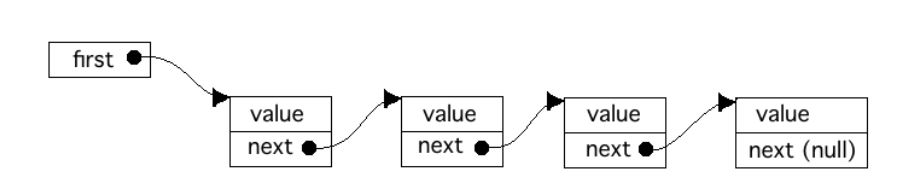
\includegraphics[width=0.5\linewidth]{immagini/singly linked list.JPG}
        \label{fig:enter-label}
    \end{figure}

    
    Adding a Node to a linked list
    \begin{enumerate}
        \item Create a new node, \texttt{newest = Node(e)}.
        \item Set \texttt{newest.next} to the current head:  \texttt{newest.next = L.head}
        \item Update \texttt{L.head} to point to \texttt{newest}.
        \item Increase the list size: \texttt{L.size=L.size+1}
    \end{enumerate}
    \begin{figure}[h!]
        \centering
        \begin{minipage}{0.45\textwidth}
          \centering
          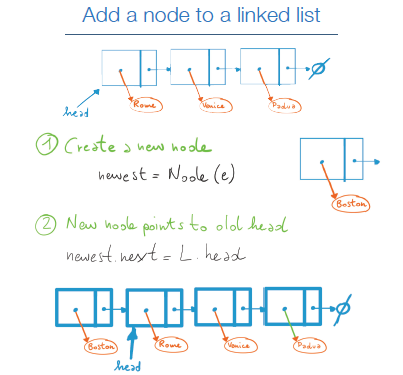
\includegraphics[width=\textwidth]{immagini/linkl1.png}
        \end{minipage}
        \hfill
        \begin{minipage}{0.45\textwidth}
          \centering
          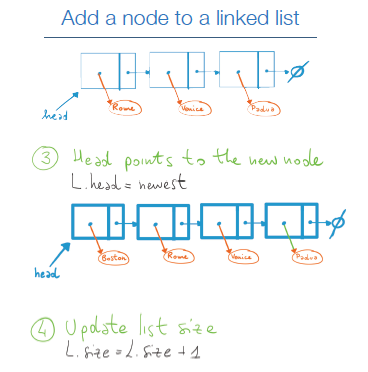
\includegraphics[width=\textwidth]{immagini/linkl2.png}
        \end{minipage}
        \label{fig:two_images}
    \end{figure}
    \newpage
    Removing a Node
    \begin{enumerate}
        \item Find the node with the value to remove (e.g., "Rome").
        \item Set \texttt{previous.next} to \texttt{current.next} and delete the current node.
    \end{enumerate}
    \begin{figure}[h!]
        \centering
        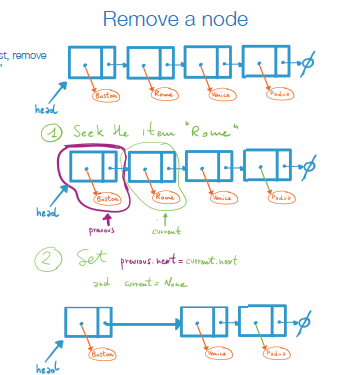
\includegraphics[width=0.5\linewidth]{immagini/linkl3.png}
    \end{figure}

    \subsection{Circularly Linked List}
    In a circularly linked list, the last node points back to the head, creating a circular structure. Be cautious with traversals as they loop infinitely.
    \begin{figure}[h]
        \centering
        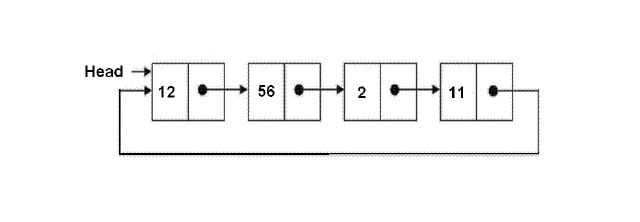
\includegraphics[width=0.8\linewidth]{immagini/circularly linked lists.JPG }
        \label{fig:enter-label}
    \end{figure}
    \newpage
    \subsection{Doubly Linked List}
    A doubly linked list has pointers in both directions, allowing traversal from both ends. It includes header and trailer nodes as sentinels, which simplify insertions.
    \begin{figure}[h!]
        \centering
        \begin{minipage}{0.7\textwidth}
          \centering
          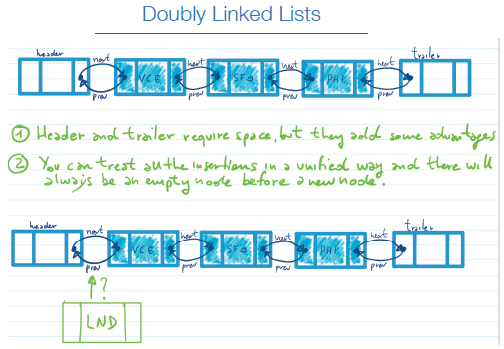
\includegraphics[width=\textwidth]{immagini/dlink1.png}
        \end{minipage}
        \hfill
        \begin{minipage}{0.7\textwidth}
          \centering
          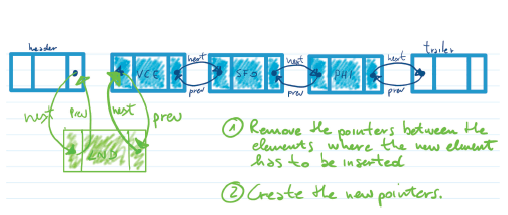
\includegraphics[width=\textwidth]{immagini/dlink2.png}
        \end{minipage}
        \label{fig:two_images}
    \end{figure}
    \subsection{Exercise: Find the Middle Node}
    Given a singly linked list of \(N\) nodes, find the middle node. If \(N\) is even, return the second middle element.
    
    \begin{itemize}
        \item Solution 1: Traverse the list and count nodes. Traverse again up to count/2 to find the middle node.
        \item Solution 2: Use two pointers, one moving twice as fast as the other. When the fast pointer reaches the end, the slow pointer is at the middle.
    \end{itemize}
    
    \subsection{Exercise: Check if a Linked List is a Palindrome}
    Given a singly linked list, check if it is a palindrome.
    
    \textbf{Solution}: Traverse the list, pushing each node onto a stack. Traverse again, popping elements from the stack and comparing each with the current node. If all match, return true.
    
    \subsection{Exercise: Reverse a Linked List}
    Given the head of a linked list, reverse the list.
    
    \textbf{Solution}:
    \begin{verbatim}
    current = head
    while current is not None:
        next = current.next
        current.next = prev
        prev = current
        current = next
    head = prev
    \end{verbatim}
    
    \subsection{Positional List}
    It is a data structure that allows us to perform arbitrary insertions and deletions or to refer to elements anywhere in a list. Numerical indexes are good, but they require to scan the entire list to find a specific element and to change dynamically when we update a list. An index does not always refer to the same element within a list. A positional list is an abstraction that provides the ability to identify the position of an element in a list.
    

    
    \section{Array vs. List-Based Data Structures}
    The complexity of those structure is different:
    \begin{itemize}
        \item Arrays: O(1)-time access to an element based on an index
        \item O(n) in a linked list to do the traversal
    \end{itemize}
    Also the storing consumption is different:
    \begin{itemize}
        \item Arrays: we may need to store 2n elements (dynamic resizing)
        \item Lists: we store n elements and n references (singly linked lists) and 2n references (doubly linked lists)
    \end{itemize}
    
    \begin{figure}[h]
        \centering
        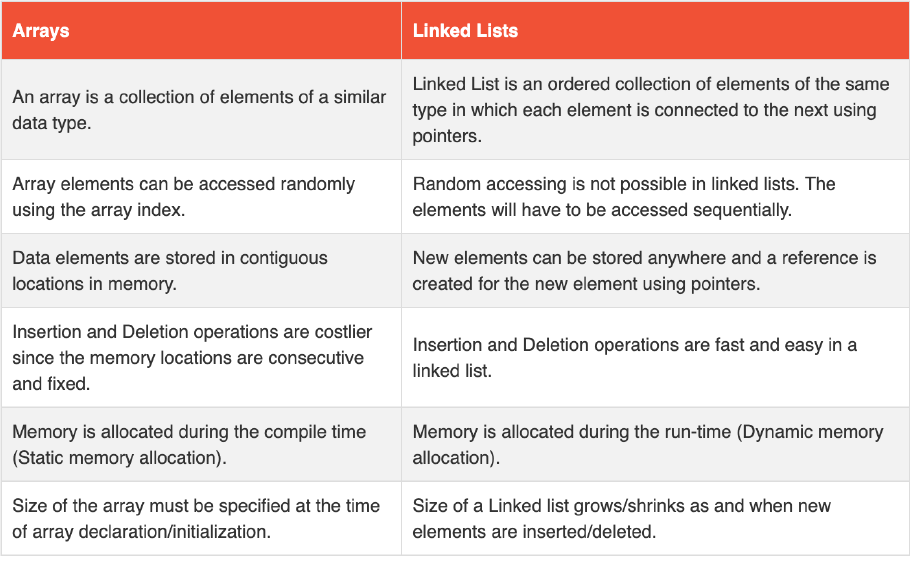
\includegraphics[width=0.9\linewidth]{immagini/06_data structure table .png}

    \end{figure}
        
    \section{Implementing Linked Lists with Arrays}

    \begin{enumerate}
        \item  Using Three Arrays: Implementation with three arrays:
                   \begin{itemize}
                       \item \texttt{next} keep the pointers to the next element.
                       \item \texttt{key} contains the actual elements.
                       \item \texttt{prev} stores the index of the previous element.
                   \end{itemize}
                Here, \texttt{L} maintains the index of the head.
        \item Using a Single Array: Represent objects in a contiguous sub-array \([j \dots k]\). Each attribute corresponds to an offset (e.g., key, next, prev), and the object's pointer is the starting index \(j\).
    \end{enumerate}
    \begin{figure}
        \centering
        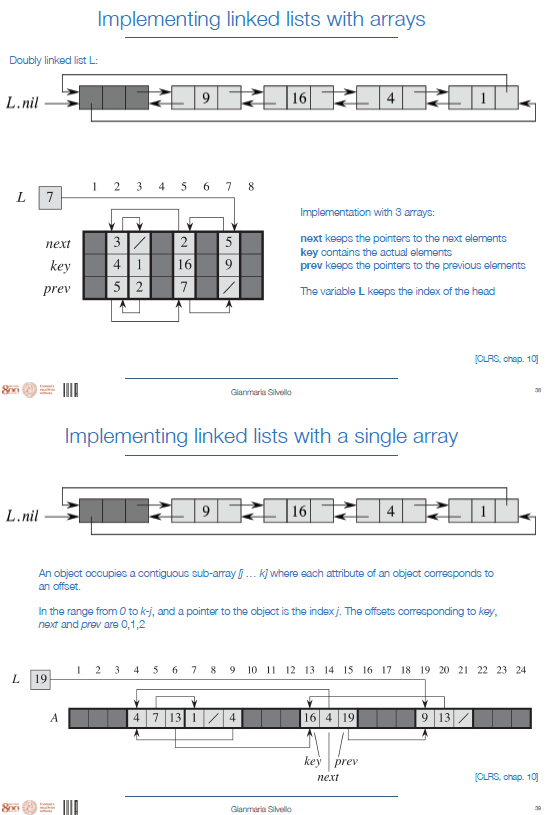
\includegraphics[width=1\linewidth]{immagini/listarray.png}
        \label{fig:enter-label}
    \end{figure}
    
    

    
    


\chapter{Trees}

\section{Introduction to Trees}
\begin{figure}[h!]
    \centering
    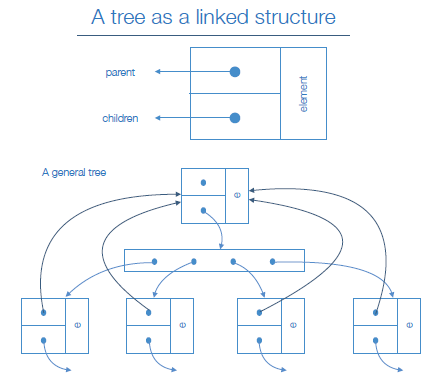
\includegraphics[width=0.75\linewidth]{immagini/general tree.png}
    \label{fig:enter-label}
\end{figure}
A \textbf{tree} is a data structure widely used to represent hierarchical relationships. It consists of nodes connected by edges and is fundamental in computer science for its structural properties. A formal tree structure satisfies the following conditions:
\begin{enumerate}
    \item It has \( n \) vertices and \( n - 1 \) edges.
    \item It is a connected graph without circuits.
    \item Any pair of vertices is connected by a unique path.
\end{enumerate}
If any of the above is true, the structure is a tree.

\section{Free Trees}
A \textbf{free tree} is a connected, acyclic, undirected graph. If a graph is acyclic but disconnected, it is termed a \textbf{forest}. Given an undirected graph \( G = (V, E) \):
\begin{itemize}
    \item If \( G \) is a free tree, any two vertices are connected by a unique path.
    \item \( G \) is connected, but if any edge is removed, the graph becomes disconnected.
    \item \( G \) has \( |E| = |V| - 1 \).
    \item \( G \) is acyclic, but adding any edge creates a cycle.
\end{itemize}

\section{Rooted Trees}
A \textbf{rooted tree} is a free tree where one of the nodes is called root.

    
\begin{figure}[h]
        \centering
        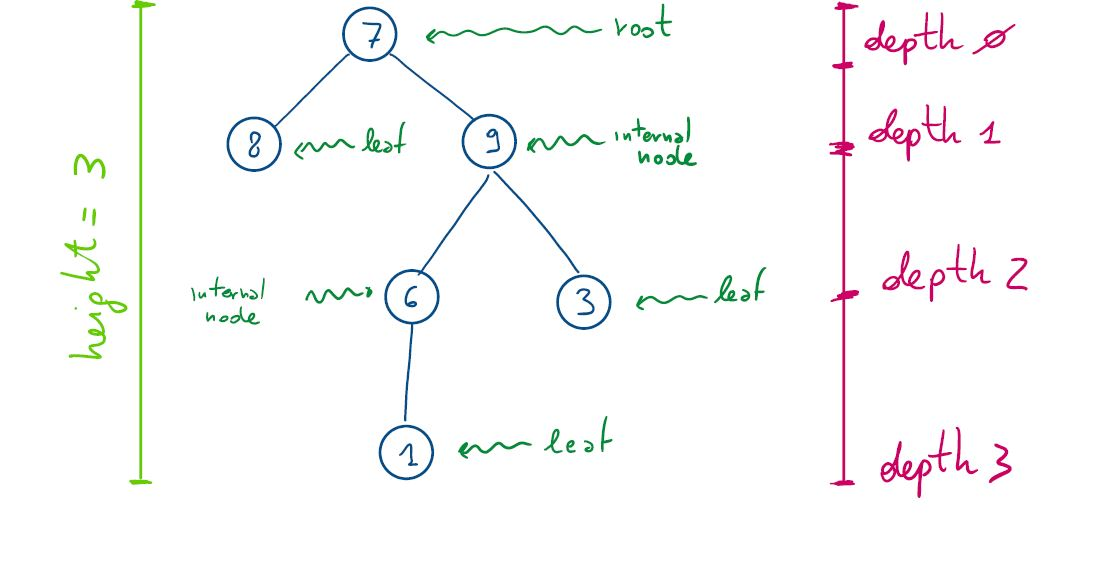
\includegraphics[width=0.5\linewidth]{immagini/rooated tree.JPG}
    \end{figure}



Each node in a rooted tree has:
\begin{itemize}
    \item \textbf{Parent}: The node directly linked above.
    \item \textbf{Child}: A node connected below.
    \item \textbf{Leaf}: A node with no children.
    \item \textbf{Internal node}: A node with at least one child.
    \item \textbf{Depth}: The level of a node from the root.
    \item \textbf{Degree}: The number of children of a node.
\end{itemize}

\subsection{Subtree and Ordered Trees}
The \textbf{subtree} rooted at \( x \) consists of \( x \) and all its descendants. In an \textbf{ordered tree}, the children of each node are arranged in a specific order (e.g.,if x has 3 children, say {y, w, z} we can say that y is the first child, w is the second child…).

\section{General Tree ADT}
The general tree Abstract Data Type (ADT) includes operations such as:
\begin{itemize}
    \item \texttt{p.element()}: Returns the element stored at position \( p \).
    \item \texttt{T.root()}: Returns the root of the tree or \texttt{None} if empty.
    \item \texttt{T.is\_root(p)}: Returns \texttt{True} if the node stored at position \( p \) is the root.
    \item \texttt{T.parent(p)}:Return the position of the parent of the node stored in \( p \).
    \item \texttt{T.num\_children(p)}: Returns the number of children of \( p \).
    \item \texttt{T.children(p)}: Generate an iteration of the children of position \( p \).
    \item \texttt{T.is\_leaf(p)} or \texttt{T.is\_external(p)}: Returns \texttt{True} if \( p \) is a leaf.
    \item \texttt{len(T)}: Returns the number of nodes.
    \item \texttt{T.is\_empty()}: Returns \texttt{True} if the tree is empty.
\end{itemize}

\section{Depth and Height of Trees}
\textbf{Depth} of a node \( p \) is the distance from \( p \) to the root. The \textbf{height} of a tree is the maximum depth among all nodes.

\subsection{Depth Calculation}
The depth of node \( p \) can be calculated using:
\begin{enumerate}
    \item Recursive method:
    \begin{verbatim}
    depth(T, p):
        if T.is_root(p):
            return 0
        else:
            return 1 + depth(T, T.parent(p))
    \end{verbatim}
    \item Iterative method:
    \begin{verbatim}
    depth(T, p):
        d = 0
        while T.parent(p) is not None:
            d += 1
            p = T.parent(p)
        return d
    \end{verbatim}
\end{enumerate}

\subsection{Height Calculation}
The height of a tree \( T \) can be computed as:
\begin{verbatim}
height(T):
    h = 0
    for each v in T.positions():
        if T.is_leaf(v):
            h = max(h, depth(T, v))
    return h
\end{verbatim}

Alternatively, using recursion:
\begin{verbatim}
height(T, p):
    if T.is_leaf(p):
        return 0
    else:
        h = 0
        for each w in T.children(p):
            h = max(h, height(T, w))
        return h + 1
\end{verbatim}

\section{Tree Traversal}
\subsection{Pre-order Traversal}
In \textbf{pre-order traversal}, the parent is visited before its children. This method is defined recursively:
\begin{verbatim}
preorder(T, p):
    visit(p)
    for each c in T.children(p):
        preorder(T, c)
\end{verbatim}
\begin{figure}[h!]
    \centering
    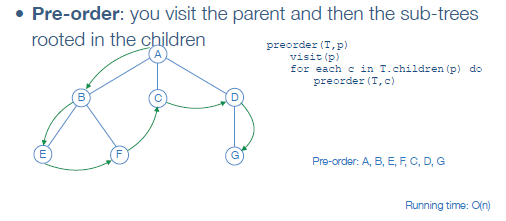
\includegraphics[width=0.75\linewidth]{immagini/tree1.png}
\end{figure}


\subsection{Post-order Traversal}
In \textbf{post-order traversal}, the children are visited before the parent.
\begin{verbatim}
postorder(T, p):
    for each c in T.children(p):
        postorder(T, c)
    visit(p)
\end{verbatim}
\begin{figure}[h!]
    \centering
    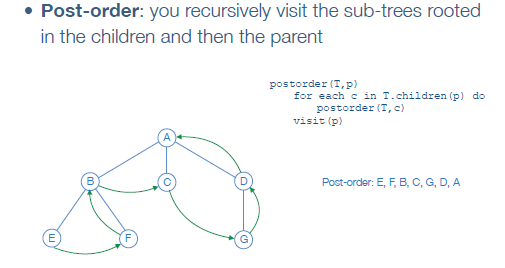
\includegraphics[width=0.75\linewidth]{immagini/tree2.png}
\end{figure}
\newpage
\subsection{Breadth-First Traversal (BFT)}
In \textbf{Breadth-First Traversal}, nodes are visited by depth level. This returns a tree. Not always it starts from left, it chooses a random child.
\begin{verbatim}
BFT(T):
    Q.enqueue(T.root())
    while not Q.is_empty():
        p = Q.dequeue()
        visit(p)
        for each c in T.children(p):
            Q.enqueue(c)
\end{verbatim}
\begin{figure}[h!]
    \centering
    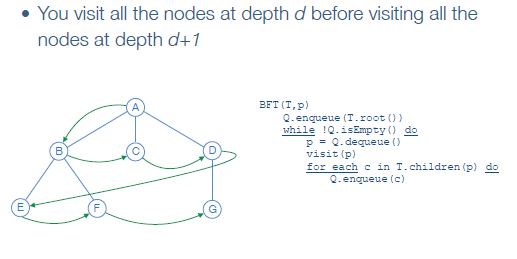
\includegraphics[width=0.75\linewidth]{immagini/tree3.png}
\end{figure}

\subsection{Exercise}
\begin{figure}[h!]
    \centering
    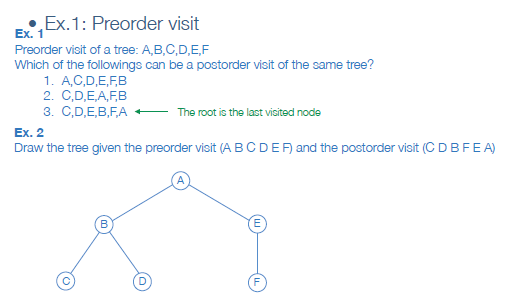
\includegraphics[width=1\linewidth]{immagini/tree4.png}
\end{figure}

\section{Binary Trees and Binary Search Trees (BST)}
A \textbf{binary tree} has each node with at most two children (left and right), the left child comes before the right child in the order of children of a node.
A binary tree is called \textbf{proper(or full)} if every node has zero or two children.
\begin{figure}[h!]
    \centering
    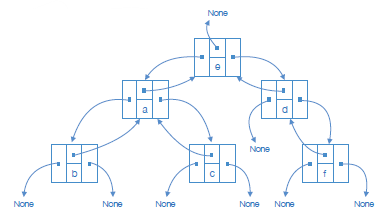
\includegraphics[width=0.75\linewidth]{immagini/tree5.png}
\end{figure}
A \textbf{Binary Search Tree (BST)} is an ordered binary tree where:
\begin{itemize}
    \item For any node \( x \), nodes in the left subtree of \( x \) have keys \( \leq x \).
    \item Nodes in the right subtree have keys \( \geq x \).
\end{itemize}
In other words: is a rooted binary tree data structure whose internal nodes each store a key greater than all the keys in
the node’s left subtree and less than those in its right subtree.

\paragraph{Complete and Full Binary Trees} There are many types of binary trees, but we will focus on two: complete and full.
\begin{itemize}
    \item \textbf{Full binary tree}: Every node has either 0 or 2 children.
    \item \textbf{Complete binary tree}: Every node has either 0 or 2 children, except for the last level, which may have some missing nodes. These nodes must be filled from left to right. A complete binary tree is also a heap.
\end{itemize}


\subsection{Binary Tree Traversal: In-Order}
In-order traversal for BST visits nodes from left to right:
\begin{verbatim}
inorder(T, x):
    if x is not None:
        inorder(T, x.left)
        visit(x)
        inorder(T, x.right)
\end{verbatim}
\begin{figure}[h!]
    \centering
    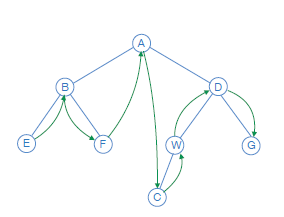
\includegraphics[width=0.6\linewidth]{immagini/tree6.png}
\end{figure}
\section{BST Operations}
Key operations in a BST include:
\begin{itemize}
    \item \textbf{Search}: Finding a node with a given key.
    \item \textbf{Minimum and Maximum}: Finding the smallest or largest element. By keeping going down to the left you will find the minimum, by going to the right you will find the maximum.
    \item \textbf{Successor and Predecessor}: Finding the next or previous node in sorted order.
\end{itemize}
\subsection{Binary Search Example: Tree-Search}
Searching for a key \( k \) in a BST starting from root node \( x \). Inputs: x is a given node where the search starts (usually the root) and k is the key to be searched in the tree. Outputs: a pointer to a node with key k or NIL if the key is not in the tree.

\begin{verbatim}
TREE-SEARCH(x, k):
    if x == NIL or k == x.key:
        return x
    if k < x.key:
        return TREE-SEARCH(x.left, k)
    else:
        return TREE-SEARCH(x.right, k)

ITERATIVE-TREE-SEARCH(x,k):
    while x!=NIL and k!=x.key() do
        if k<x.key
            x = x.left
        else
            x = x.right
    return x
\end{verbatim}

\begin{figure}[h!]
    \centering
    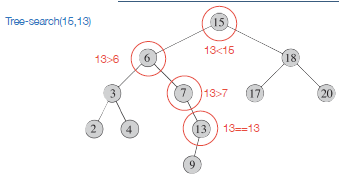
\includegraphics[width=0.75\linewidth]{immagini/tree7.png}
\end{figure}
The nodes encountered during the process form a path downward from the root, thus we visit a number of nodes which equals the height of the node k in the tree. Complexity: O(h) where h is the height
\newpage Exercise: Suppose we have numbers between 1 and 1000 in a binary search tree, and we want to search for the number 364. Which of the following sequences cannot be the sequence of nodes examined?
\begin{itemize}
    \item 1,252,401,398,330,344,397,364
    \item 924,220,911,244,898,258,362,364
    \item 925,202,911,240,912,245,364
\end{itemize}
There answer is the third option since 912 cannot belong to the left subtree of 911.

\subsection{Successor: Property}
Given a binary search tree \( T \) and \(x, y \) in \( T \) 
Given a binary search tree T and x,y in T, then \( y \) is a successor of \( x \) if \( y.key>x.key \) and there not exist a
 \( z \) in \( T \) such that \(  y.key> z.key >x.key\).  $\\$
 
\textbf{Property:} Consider a binary search tree T whose keys are distinct. If the right subtree of a node \(x\) in \(T\) is empty and \(x\) has a successor \(y\), then \(y\) is the lowest ancestor of \(x\) whose left child is also an ancestor-orself
of \(x\).
Note: in this case we consider a node to be an ancestor of itself.
The running time is O(h) since we either follow a simple path downwards or a simple path upwards.
\begin{figure}[h!]
    \centering
    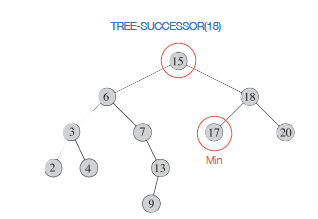
\includegraphics[width=0.75\linewidth]{immagini/tree8.png}
\end{figure}

    




\chapter{Hash Tables}

\section{Direct-Address Table}
Direct addressing is a simple and efficient method when the universe \( U \) of possible keys is relatively small. A direct-address table \( T \) is an array where:
\[
T[i] = \text{value associated with key } i
\]
Given \( U = \{0, 1, \dots, m-1\} \), \( T \) is of size \( m \).

\subsection{Operations}
\begin{figure}[H]
    \centering
    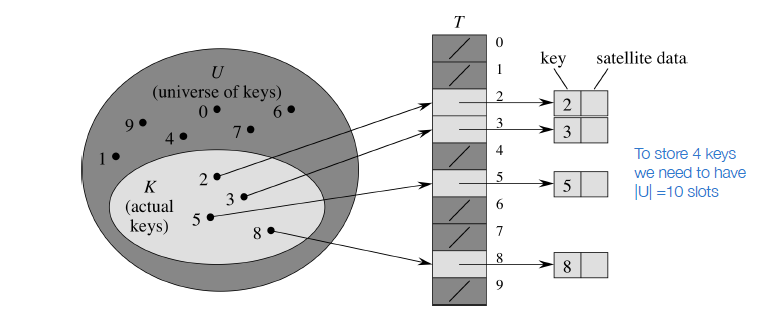
\includegraphics[width=0.75\linewidth]{direct-adress table.png}
    \label{fig:enter-label}
\end{figure}

\begin{itemize}
    \item \texttt{Direct-Table-Search(T, k):} Returns \( T[k] \), \( O(1) \).
    \item \texttt{Direct-Table-Insert(T, x):} Returns \( T[x.key] = x \), \( O(1) \).
    \item \texttt{Direct-Table-Delete(T, x):} Returns \( T[x.key] = NIL \), \( O(1) \).
\end{itemize}



While the first is a time-efficient approach, the 2nd and 3rd approaches becomes space-inefficient if \( |U| \gg |K| \), where \( K \) is the actual set of keys.

\section{Hash Tables}
Hash tables address the inefficiency of direct addressing by using a hash function \( h: U \to \{0, 1, \dots, m-1\} \), which maps keys to slots of a fixed-size table \( T[0,1,...,m-1] \). $\\$



\title{Hash Tables Overview}

\begin{itemize}
    \item Hash tables use a table size proportional to \( |K| \), losing the direct address ability.
    \item Direct-addressing maps \( k \to T[k] \), but wastes space if \( U \) (key space) is large.
    \item A \textbf{hash function} \( h \) maps keys to table slots:
    \[
    h : U \to \{ 0, 1, \dots, m-1 \}
    \]
    \item Keys are placed in \( T[h(k)] \) instead of \( T[k] \), optimizing storage.
\end{itemize}




\subsection{Hash Function}
A hash function should:
\begin{itemize}
    \item Be simple and fast to compute.
    \item Avoid collisions.
    \item Distribute keys evenly among cells.
\end{itemize}
Example: Let \( h(k) = k \mod 6 \), \( T[0..5] \):
\begin{itemize}
    \item Insert 7: \( 7 \mod 6 = 1 \)
    \item Insert 18: \( 18 \mod 6 = 0 \)
    \item Insert 41: \( 41 \mod 6 = 5 \)
    \item Insert 34: \( 34 \mod 6 = 4 \)
    \item Insert 10: \( 10 \mod 6 = 4 \) (collision with \( 34 \)).
\end{itemize}

\begin{figure}[H]
    \centering
    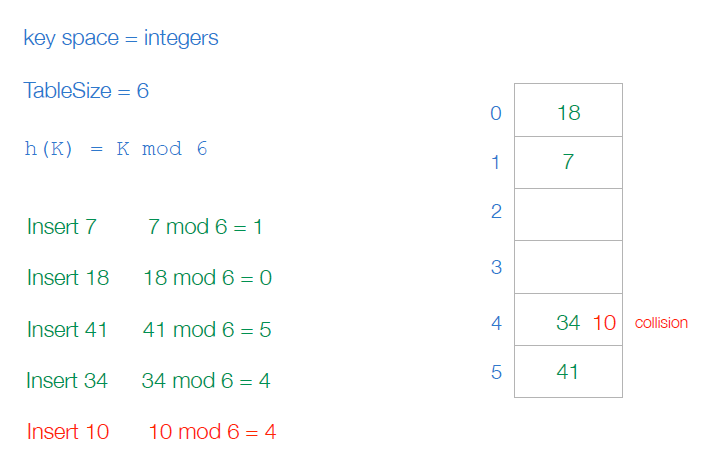
\includegraphics[width=0.75\linewidth]{hash function exam.png}
    \label{fig:enter-label}
\end{figure}


\section{Collision Resolution Strategies}

\subsection{Separate Chaining}
Collisions are resolved by maintaining a linked list at each slot.
\begin{itemize}
    \item \texttt{Insert:} \( O(1) \) if the element is unique, otherwise \( O(1 + \text{SEARCH}) \).
    \item \texttt{Search:} Proportional to the list length at the slot.
    \item \texttt{Delete:} \( O(1 + \text{SEARCH}) \).
\end{itemize}
Performance depends on the \textbf{load factor} \( \alpha = \frac{n}{m} \), where \( n \) is the number of elements and \( m \) is the size of the table. $\\$
The load factor is the average number of elements stored in a hash table where \(\alpha \in[0,1]\). Therefore the worst case is $\Theta (n)$.

\begin{figure}[H]
    \centering
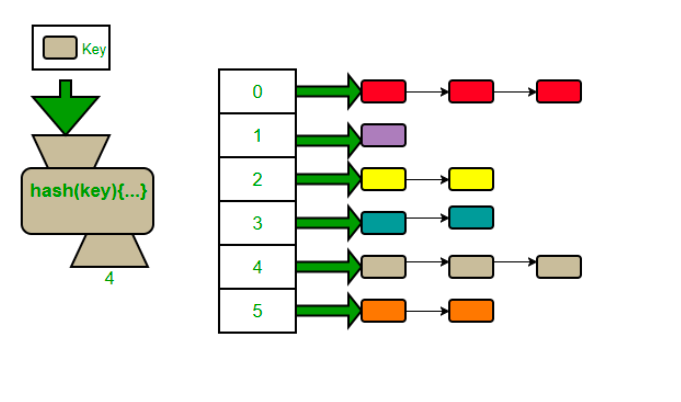
\includegraphics[width=0.75\linewidth]{separe chaining.png}
\end{figure}



\section{Simple Uniform Hashing}

\begin{itemize}
    \item For \( j = 0, 1, \dots, m-1 \), let \( T[j] \) denote the list corresponding to slot \( j \) with length \( n_j \), such that:
    \[
    n = n_0 + n_1 + \dots + n_{m-1}.
    \]
    \item The expected value of \( n_j \) is:
    \[
    \mathbb{E}[n_j] = \alpha = \frac{n}{m},
    \]
    where \( \alpha \) is the load factor.
    \item The average running time for a successful search in a hash table using chaining and assuming simple uniform hashing is:
    \[
    \Theta(1 + \alpha).
    \]
    \item If \( m \) is proportional to \( n \), then \( n = O(m) \) and:
    \[
    \alpha = \frac{n}{m} = \frac{O(m)}{m} = O(1).
    \]
\end{itemize}



\subsection*{Division Method}
The hash function is defined as:
\[
h(k) = k \mod m
\]
where \( k \) is the key, and \( m \) is the table size. 
\begin{itemize}
    \item Choose \( m \) as a prime number not close to a power of 2.
    \item Example: For \( n = 2000 \) keys and 3 collisions per list, estimate \( m \approx 666 \). A good choice is \( m = 701 \).
\end{itemize}

\subsection{Alternative Methods}
\begin{itemize}
    \item \textbf{Multiplication Method}:
    \[
    h(k) = \lfloor m \cdot (kA \mod 1) \rfloor
    \]
    where \( A \approx 0.61803 \) (Knuth's suggestion).
   \item \textbf{Squaring Method}:
    \begin{itemize}
        \item Square the key and extract middle bits.
        \item Often use \( m = 2^p \) for simpler computation.
    \end{itemize}

\end{itemize}







\subsection{Open Addressing}
Instead of linked lists (which requires the implementation of a second data structure), all data is stored directly in the table (we need a bigger table and the load factor should be below 0.5). When a collision occurs, alternative cells are probed until an empty slot is found.
Strategies include:
\begin{enumerate}
    \item \textbf{Linear Probing:} \( h_i(k) = (h(k) + i) \mod m \).
    \item \textbf{Quadratic Probing:} \( h_i(k) = (h(k) + i^2) \mod m \).
    \item \textbf{Double Hashing:} \( h_i(k) = (h(k) + i \cdot g(k)) \mod m \), where \( g \) is a second hash function.
\end{enumerate}

\subsubsection{Linear Probing Example}

\textbf{Probe Sequence:}  
When resolving collisions using linear probing, the probe sequence is defined as follows:

\begin{itemize}
    \item \( 0^\text{th} \) probe: \( h(k) = k \mod \text{TableSize} \),
    \item \( 1^\text{st} \) probe: \( (h(k) + 1) \mod \text{TableSize} \),
    \item \( 2^\text{nd} \) probe: \( (h(k) + 2) \mod \text{TableSize} \),
    \item \(\dots\),
    \item \( i^\text{th} \) probe: \( (h(k) + i) \mod \text{TableSize} \).
\end{itemize}
\textbf{Key Properties:}
\begin{itemize}
    \item A function of \( i \) is added to the original hash value to resolve collisions.
    \item Any key that hashes into an existing cluster:
    \begin{enumerate}
        \item Will require multiple attempts to resolve the collision.
        \item Will contribute to the cluster, increasing its size.
    \end{enumerate}
\end{itemize}


\begin{figure}[H]
    \centering
    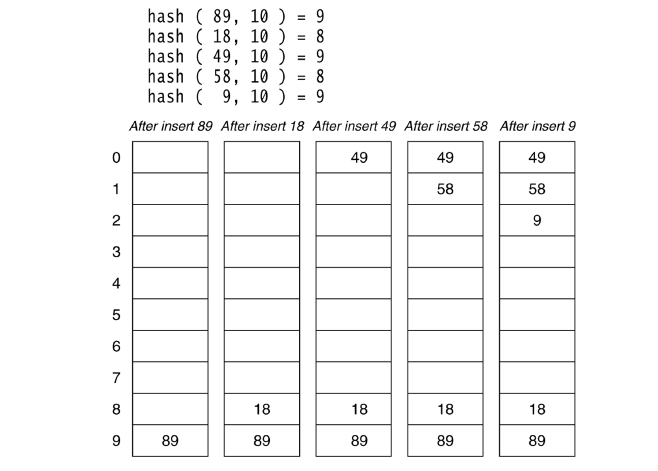
\includegraphics[width=0.75\linewidth]{linear probing.png}
\end{figure}




\subsection{Open Addressing: Search and Insertion}  

In open addressing, the search process uses the same probe sequence as insertion. For example, searching for 58 takes 4 probes, while searching for 19 takes 5.  

The average number of cells examined during insertion with linear probing is:  
\[
\frac{1 + \frac{1}{(1 - \alpha)^2}}{2}
\]  
The cost of successfully searching for an element equals the cost of its insertion.  

When the table is half full (\( \alpha = 0.5 \)), the average insertion cost is 2.5, and this remains true for future searches.  

For unsuccessful searches, the average cost is:  
\[
\frac{1 + \frac{1}{(1 - \alpha)^2}}{2}
\]  
For successful searches:  
\[
\frac{1 + \frac{1}{1 - \alpha}}{2}
\]  
At \( \alpha = 0.5 \), insertion typically examines 2.5 cells.  

Primary clustering worsens as the table fills, but when half empty, the effect is minimal.  

\subsection{Linear Probing Example:}
\begin{figure}[H]
    \centering
    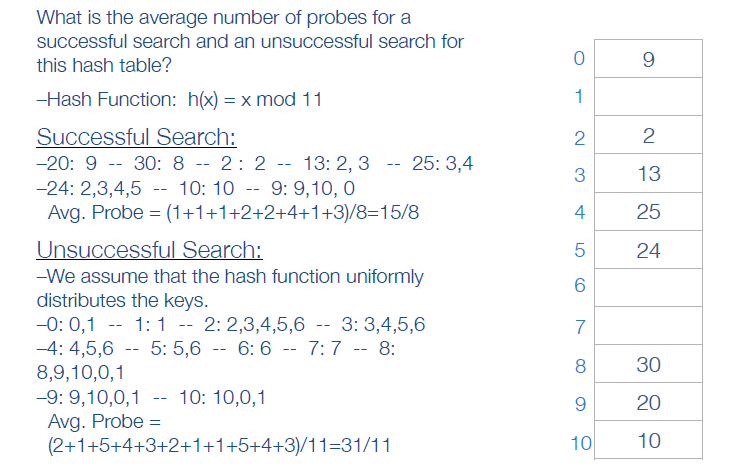
\includegraphics[width=0.75\linewidth]{LP example.png}
\end{figure}

\subsubsection{Primary Clustering}
It works pretty well for an empty table and gets worse as the table fills up.
If a bunch of elements hash to the same spot, they clash with each other. But, worse, if a bunch of elements hash to the same area of the table, they keep clashing! (Even though the hash function isn’t producing lots of collisions!)$\\$
This phenomenon is called primary clustering and Linear probing suffers from \textbf{primary clustering}, where elements form clusters that grow, increasing the likelihood of future collisions.

\begin{figure}[H]
    \centering
    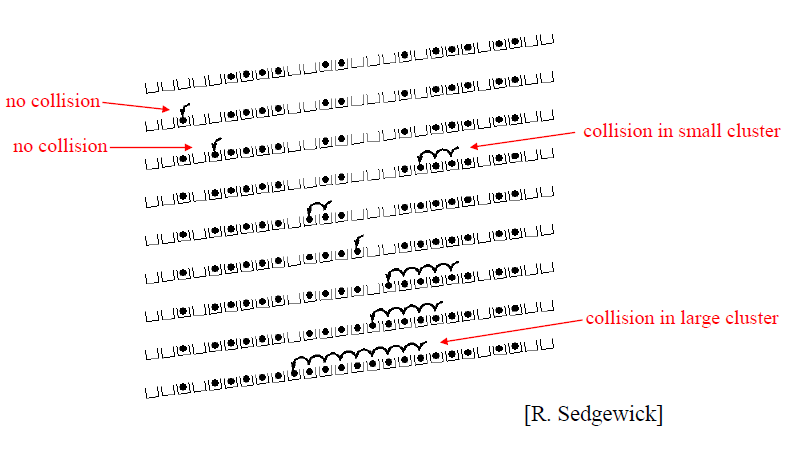
\includegraphics[width=0.75\linewidth]{primary clustering.png}
    \caption{Enter Caption}
    \label{fig:enter-label}
\end{figure}

\subsubsection{Quadratic Probing}
\textbf{Reduces Primary Clustering:} Keys that hash to nearby slots do not follow the same probe sequence.

Reduces clustering but may encounter \textbf{secondary clustering} where keys hashing to the same slot follow identical probe sequences. \( h_i(k) = (h(k) + i^2) \mod m \).

There are cases in which, due to probing, there is no available spot. If there are numbers in the same place those will cause infinite collisions. For example
\begin{align}
47 \hspace{1mm} \text{mod} \hspace{1mm} 7 =  5 \rightarrow & 5+(i^2) \\
                                               \rightarrow & 5+(i+1)^2 \\
                                               \rightarrow & 5+(i+2)^2 ...    
\end{align}
but also
\begin{align}
75 \hspace{1mm} \text{mod} \hspace{1mm} 7 =  5 \rightarrow & 5+(i^2) \\
                                               \rightarrow & 5+(i+1)^2 \\
                                               \rightarrow & 5+(i+2)^2 ...    
\end{align}
\begin{figure}[h!]
    \centering
    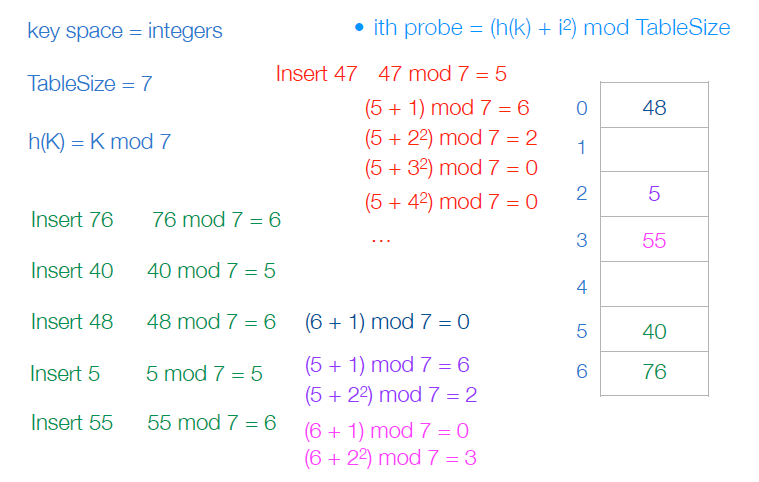
\includegraphics[width=0.75\linewidth]{quadratic probing example.png}
    \label{fig:enter-label}
\end{figure}

\subsubsection{Double Hashing Example}
Hash function \( h(k) = k \mod 7 \), \( g(k) = 5 - (k \mod 5) \):
Insert 76, 93, 40, 47, 10, 55. \newline
\textbf{Table Size:}  
 Optimal load factor \( \alpha = \frac{1}{2} \) (table twice as large as expected elements).  \newline
\textbf{Probe Calculation} Next probe:  
    \[
    (i+1)^2 - i^2 = 2i + 1
    \]
For \( \alpha < \frac{1}{2} \), an empty slot is always found. If \( \alpha > \frac{1}{2} \), a slot may not exist.  

\begin{figure}[h!]
    \centering
    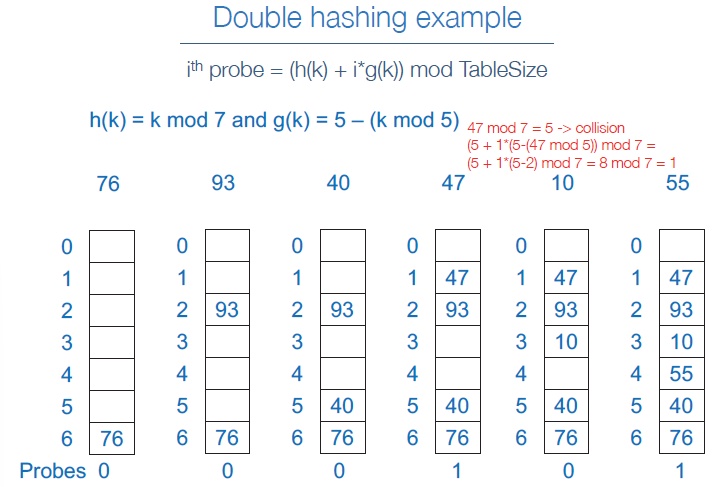
\includegraphics[width=0.75\linewidth]{immagini/doublehahing.png}
\end{figure}
\section{Rehashing}
When the table is too full (\( \alpha > 0.5 \)), rehashing is required:
\begin{itemize}
    \item Create a new table, typically twice as large.
    \item Recompute hash values for all non-deleted keys.
\end{itemize}
Rehashing costs \( O(n) \) but occurs infrequently.

\section{Python Hash Tables}
Python dictionaries are implemented as hash tables using \textbf{open addressing:}  with random probing. Collisions are handled by comparing both the hash and the key. If the hash and key match, the entry is skipped, otherwise probing continues until an empty slot is found. 
$\\$

When a new dictionary is created, it starts with 8 slots. The table resizes when it becomes two-thirds full to maintain efficiency. Each slot can store one entry, and if the slot is occupied, Python checks for a match using the == operator (not is). If no match is found, random probing selects the next slot in a pseudo-random order, continuing until the entry is placed. 
$\\$

This design ensures efficient insertion, lookup, and handling of collisions, keeping Python dictionaries fast and reliable.

\chapter{Heaps and Heapsort}

\section{Introduction to Heaps}
\begin{figure}[h!]
    \centering
    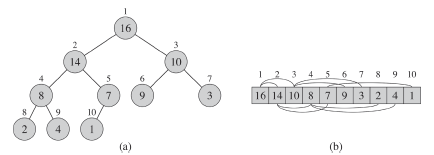
\includegraphics[width=0.75\linewidth]{immagini/heap1.png}
\end{figure}
Heaps are a foundational data structure in computer science used for efficient sorting and priority management. They offer:
\begin{itemize}
    \item Sorting algorithm with \( O(n \log n) \) complexity.
    \item An in-place sorting mechanism.
    \item A design that uses a specific data structure to manage information during execution.
    \item Applications in sorting (\textit{Heapsort}) and other efficient structures like priority queues.
\end{itemize}

\section{The Heap Data Structure}
A \textbf{heap} is an array-based data structure often represented as a nearly complete binary tree:
\begin{itemize}
    \item The tree is filled level by level, with the last level filled from left to right. The first element will always be the root.
    \item An array \( A \) representing a heap has attributes:
    \begin{itemize}
        \item \texttt{length[A]}: Total size of the array.
        \item \texttt{heap-size[A]}: Number of elements in the heap, with \( \texttt{heap-size[A]} \leq \texttt{length[A]} \).
    \end{itemize}
\end{itemize}
\begin{figure}[H]
    \centering
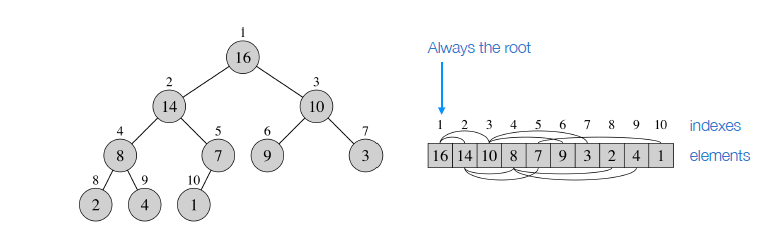
\includegraphics[width=0.8\linewidth]{Heap structure.png}
    \caption{}
    \label{fig:enter-label}
\end{figure}


\subsection{Heap Properties}
\begin{itemize}
    \item The root is stored at \( A[1] \).
    \item For an element at index \( i \):
    \begin{itemize}
        \item Parent: \( A[\lfloor i/2 \rfloor] \).
        \item Left child: \( A[2i] \).
        \item Right child: \( A[2i+1] \).
    \end{itemize}
    \item \textbf{Max-heap property:} \( A[\text{parent}(i)] \geq A[i] \).
    \item \textbf{Min-heap property:} \( A[\text{parent}(i)] \leq A[i] \).
\end{itemize}
\subsection{exercise}
\begin{figure}[h!]
    \centering
    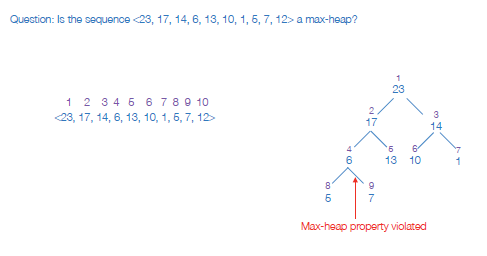
\includegraphics[width=1\linewidth]{immagini/heap2.png}
\end{figure}

\begin{figure}[H]
    \centering
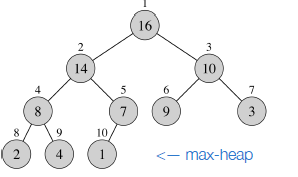
\includegraphics[width=0.5\linewidth]{heap prop.png}
    \label{fig:enter-label}
\end{figure}


\section{Max-Heapify}
The \textbf{Max-Heapify} operation ensures the max-heap property by adjusting the heap from a specific index downward.

\subsection{Algorithm: Max-Heapify}
\begin{verbatim}
MAX-HEAPIFY(A, i)
l = left(i)
r = right(i)
if l <= heap-size[A] and A[l] > A[i] then
    largest = l
else
    largest = i
if r <= heap-size[A] and A[r] > A[largest] then
    largest = r
if largest != i then
    exchange A[i] with A[largest]
    MAX-HEAPIFY(A, largest)
\end{verbatim}

\textbf{Complexity:} \( O(\log n) \), proportional to the height of the tree.
\begin{figure}[h!]
    \centering
    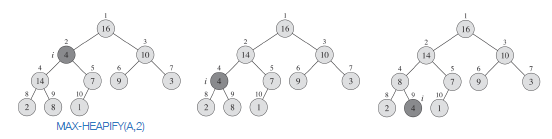
\includegraphics[width=1\linewidth]{immagini/heap3.png}
\end{figure}
\section{Building a Max-Heap}
\textbf{BUILD-MAX-HEAP} constructs a max-heap from an unordered array.

\subsection{Algorithm: Build-Max-Heap}
\begin{verbatim}
BUILD-MAX-HEAP(A)
heap-size[A] = length[A]
for i = floor(length[A]/2) downto 1 do
    MAX-HEAPIFY(A, i)
\end{verbatim}
\textbf{Complexity:} \( O(n) \). This is more efficient than the naive \( O(n \log n) \) bound because most heap levels have fewer nodes. \newline
\textbf{How does it work?} The algorithm starts checking from the element $\lfloor len(A)/2 \rfloor$ and then works its way back up. In each step, it fixes everything before moving on. Note that the system always looks down and not up, using \textbf{MAX-HEAPIFY(A,1)} we always consider the first element that looks at the entire graph.
\subsection{Exercise}
    \begin{figure}[h!]
        \centering
        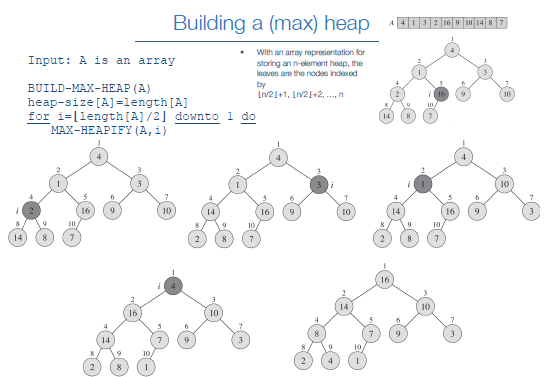
\includegraphics[width=1\linewidth]{immagini/heap4.png}
    \end{figure}
The loop could not go from 1 to floor(length[A]/2) because it could not guarantee the maxheap property. E.g. A [2,1,1,3] then MAX-HEAPIFY won’t exchange 2 with it’s children (1’s). However, when MAX-HEAPIFY is called on the left child, 1, it will swap 1 with 3. This violates the max-heap property because now 2 is the parent of 3. An upper bound of the running time is O(n log n) because MAX-HEAPIFY costs O(log n) and we call it O(n) times. It is possible to derive a tighter upper bound by observing that the time required by MAXHEAPIFY varies with the height of the node and most heights are small. It can be proved that BUILD-MAX-HEAP run in O(n).
    
\section{Heapsort}
\textbf{Heapsort} is a sorting algorithm that uses a heap to organize data efficiently.

\subsection{Algorithm: Heapsort}
\begin{verbatim}
HEAPSORT(A)
BUILD-MAX-HEAP(A) #O(n)
for i = len(A) downto 2 do #O(n-1)
    exchange A[1] with A[i] #O(1)
    A.heap-size = A.heap-size - 1 #O(1)
    MAX-HEAPIFY(A, 1) #O(logn)
\end{verbatim}
\textbf{Complexity:} \( O(n) + O((n-1)(\log n)) = O(n \log n) \).

\subsection{Exercise 1}
    \begin{figure}[h!]
        \centering
        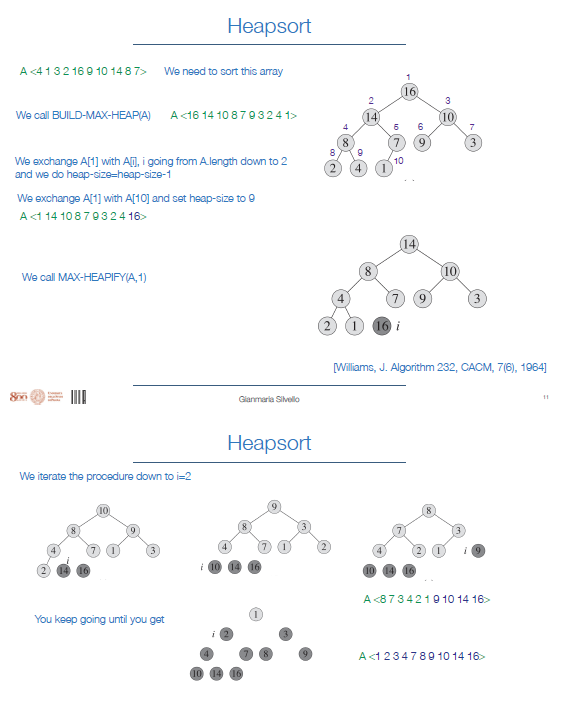
\includegraphics[width=1\linewidth]{immagini/heap5.png}
    \end{figure}
\newpage
\subsection{Exercise 2}
    \begin{figure}[h!]
        \centering
        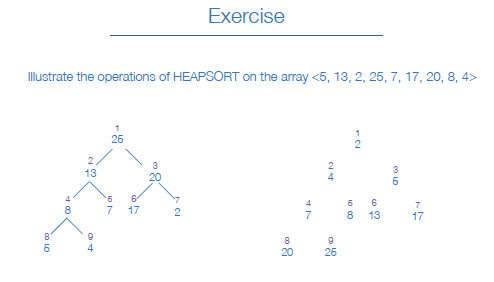
\includegraphics[width=0.8\linewidth]{immagini/heap6.png}
    \end{figure}

\section{Priority Queues}
Priority queues are abstract data structures for managing elements with associated priorities.

\subsection{Operations}
\begin{itemize}
    \item \texttt{INSERT(S, x)}: Add element \( x \) to \( S \).
    \item \texttt{MAXIMUM(S)}: Return the element with the maximum key.
    \item \texttt{EXTRACT-MAX(S)}: Remove and return the element with the maximum key.
    \item \texttt{INCREASE-KEY(S, x, k)}: Increase the key of \( x \) to \( k \) (\( k \geq \) current key).
\end{itemize}

\subsection{Complexity}
If implemented with a heap:
\begin{itemize}
    \item \texttt{INSERT(S, x)}: \( O(\log n) \).
    \item \texttt{MAXIMUM(S)}: \( O(1) \).
    \item \texttt{EXTRACT-MAX(S)}: \( O(\log n) \).
\end{itemize}
\chapter{Introduction to Dynamic Programming}

Dynamic programming (DP) is a method to solve complex problems by breaking them into smaller overlapping subproblems and building up solutions incrementally. It is essentially a technique for optimizing certain inefficient recursive algorithms by caching intermediate results for later reuse. 

\subsection{Key Concepts}
\begin{itemize}
    \item \textbf{Inefficiency in Recursion}: Many recursive algorithms are inefficient because they repeatedly solve the same subproblems.
    \item \textbf{Caching Results}: By storing intermediate results in a table (e.g., a hash table), we can avoid recalculating the same subproblem multiple times.
    \item \textbf{Efficiency}: This approach skips repeated recursive calls, speeding up the algorithm significantly.
\end{itemize}

\section{Elements of Dynamic Programming}

To effectively apply dynamic programming, the problem should have the following properties:

\begin{itemize}
    \item \textbf{Simple Subproblems}: The problem can be broken into smaller subproblems with the same structure.
    \item \textbf{Optimal Substructure}: The optimal solution of the overall problem depends on the optimal solutions of its subproblems.
    \item \textbf{Overlapping Subproblems}: Subproblems are solved multiple times during the computation.
\end{itemize}

\section{Case Study: Rod Cutting}
\begin{figure}[h!]
    \centering
    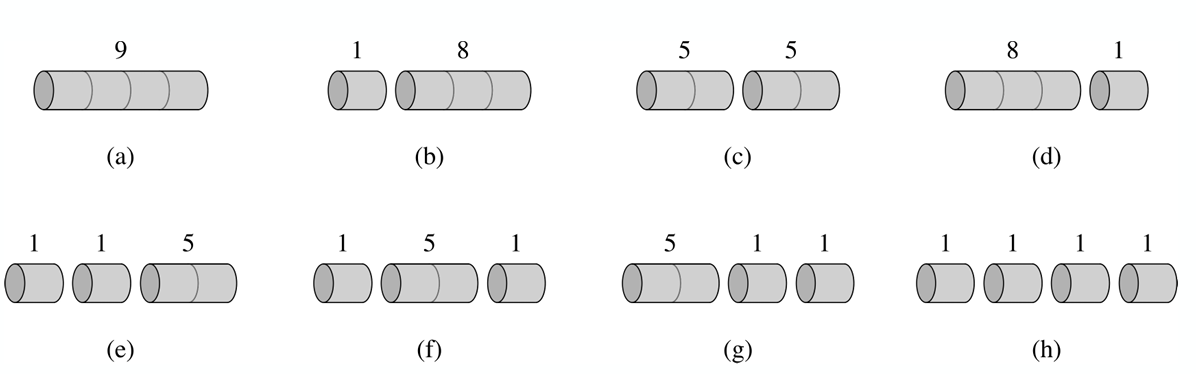
\includegraphics[width=1\linewidth]{immagini//capitolo 13/13_2.png}
    \caption{Enter Caption}
    \label{Example 1, here we show eight possible ways to cut a rod of lenght 4, the prices are shown on top}
\end{figure}
\subsection{Problem Statement}
Given a rod of length \(n\) inches and a table of prices \(p_i\) for rods of length \(i\), determine the maximum revenue obtainable by cutting the rod into smaller pieces and selling them.
\begin{figure}[h!]
    \centering
    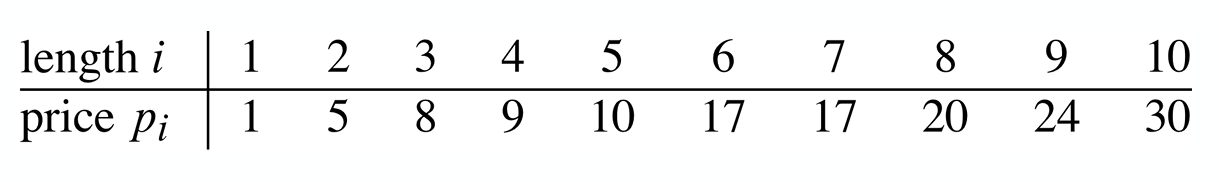
\includegraphics[width=1\linewidth]{immagini//capitolo 13/13_1.png}
    \caption{Another example of possible table of prices}
    \label{fig:enter-label}
\end{figure}
\textbf{Key Points:}
\begin{itemize}
    \item Rod cuts are integral lengths, and cutting incurs no cost.
    \item The solution involves finding the optimal way to cut the rod to maximize revenue.
\end{itemize}
The general formula for the maximum revenue \(r_n\) is:
\[
r_n = \max \big( p_n, r_1 + r_{n-1}, r_2 + r_{n-2}, \dots, r_{n-1} + r_1 \big) = \max_{1 \leq i \leq n} \big( p_i + r_{n-i} \big)
\]

\begin{itemize}
    \item \( p_n \): This represents the revenue obtained by selling the rod as is, without making any cuts. It is the simplest case.
    \item For the other \( n-1 \) arguments in the maximization formula, these correspond to the maximum revenue obtained by making an initial cut of the rod into two pieces of size \( i \) and \( n-i \), for each \( i = 1, 2, \dots, n-1 \).
    \item Once the rod is cut into two pieces, the revenues \( r_i \) and \( r_{n-i} \) are obtained by optimally cutting up those two pieces further.
    \item After making the first cut, the two resulting pieces can be treated as independent instances of the rod-cutting problem.
    \item The overall optimal solution incorporates the optimal solutions to these two related subproblems, maximizing the revenue from each of the two pieces. This ensures that the global solution is composed of optimal solutions to the subproblems.
\end{itemize}
In summary, the rod-cutting problem uses a divide-and-conquer strategy where the maximum revenue for a rod of length \( n \) is calculated by exploring all possible initial cuts, solving the subproblems for each resulting piece, and combining the results to achieve the maximum total revenue.

\subsection{Recursive Algorithm}

\begin{verbatim}
CUT-ROD(p, n):
    if n == 0:
        return 0  # No revenue is possible for a rod of length 0, so CUT-ROD return 0
    q = -infty
    for i = 1 to n:
        q = max(q, p[i] + CUT-ROD(p, n - i))  # Recursive call on the second piece
    return q
\end{verbatim}

\textbf{Explanation of the Code:}
\begin{itemize}
    \item \texttt{CUT-ROD} recursively computes the maximum revenue for a rod of length \(n\).
    \item The loop considers all possible first cuts (length \(i\)) and recursively solves for the remaining rod of length \(n-i\).
    \item It calls itself recursively many times with the same parameter values. 
    \item The result is the maximum revenue over all possible first cuts.
    \item This algorithm has an exponential running time \(T(n) = 2^n\), as it repeatedly solves the same subproblems.
\end{itemize}

\begin{figure}[h!]
    \centering
    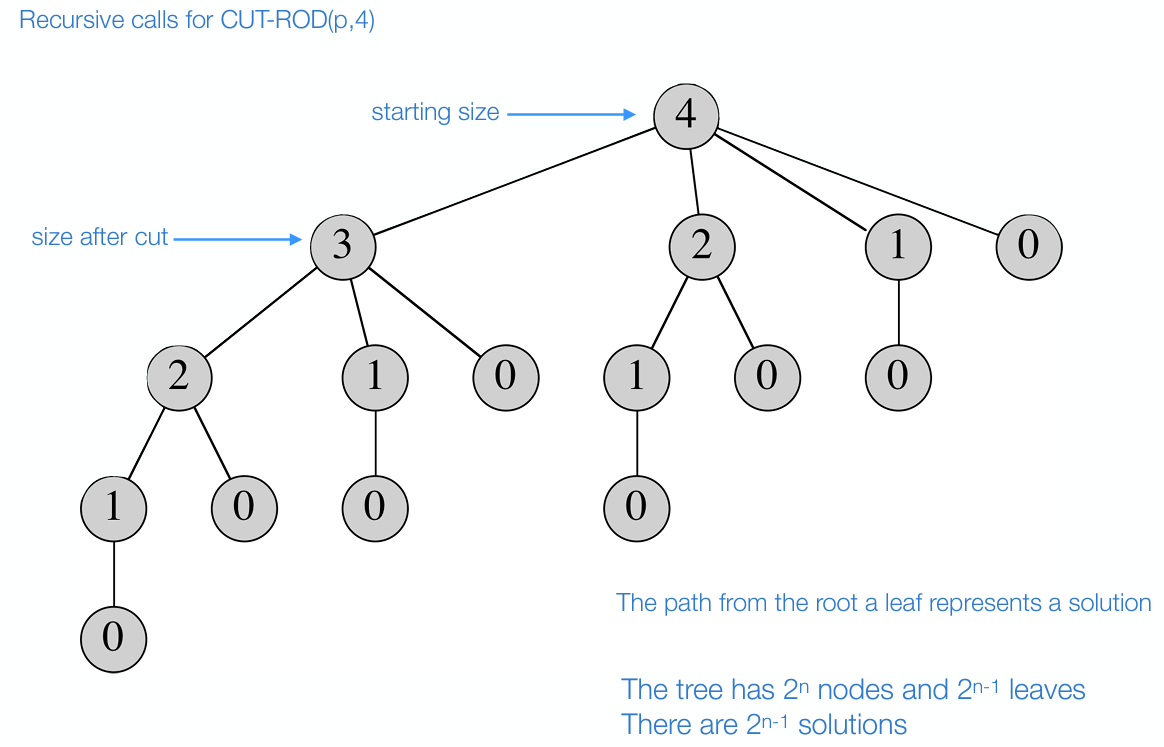
\includegraphics[width=1\linewidth]{immagini//capitolo 13/13_3.png}
    \label{CUT}
\end{figure}

\section{Improving Efficiency with Dynamic Programming}

\textbf{Key Idea:} Organize the algorithm to solve each subproblem only once, storing the solution in an appropriate data structure for reuse.

\begin{itemize}
    \item Use a data structure (e.g., array or hash table) to store solutions to subproblems.
    \item Retrieve stored solutions whenever a previously solved subproblem is encountered.
    \item Trade-off: Use more memory to store solutions but significantly reduce computation time.
\end{itemize}
\textbf{Performance:} Dynamic programming reduces the time complexity to polynomial when:
\begin{itemize}
    \item The input size is polynomial.
    \item The number of distinct subproblems is polynomial.
    \item Each subproblem can be solved in polynomial time.
\end{itemize}


\section{Memoization}

Memoization is a technique used in dynamic programming to store the solutions of subproblems to avoid redundant computations. There are two primary approaches to memoization. Both approaches have equivalent running times, but their implementations differ. Note that \textbf{memoization} is not the same as \textbf{memorization}.

\subsection{Top-Down Memoization}
In this approach, we solve the problem recursively in the usual way but store the solutions to subproblems as we compute them. This ensures that whenever we encounter a previously solved subproblem, we can simply retrieve the stored solution.

\subsection{Bottom-Up Memoization}
In this approach, we explicitly define the subproblems, order them by size in increasing order, and solve them iteratively. The solutions to smaller subproblems are used to solve larger ones. This approach avoids recursion and generally has lower constant factors compared to the top-down approach. This strategy usually has lower constant factors.



\section{Top-Down Memoization: Implementation}

\begin{verbatim}
MEMOIZED-CUT-ROD(p, n):
    let r[0, ..., n] be a new array
    for i = 0 to n:
        r[i] = -infinity
    return MEMOIZED-CUT-ROD-AUX(p, n, r)

MEMOIZED-CUT-ROD-AUX(p, n, r):
    if r[n] >= 0:  # Check for the stored solution
        return r[n]
    if n == 0:
        q = 0
    else:
        q = -infinity
        for i = 1 to n:
            q = max(q, p[i] + MEMOIZED-CUT-ROD-AUX(p, n - i, r))
    r[n] = q  # Store the solution for n
    return q
\end{verbatim}





\begin{figure}[h]
    \centering
    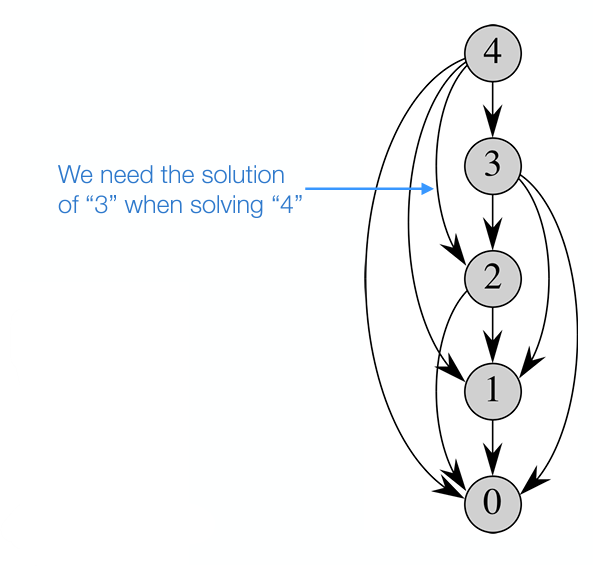
\includegraphics[width=0.75\linewidth]{immagini//capitolo 13/13_4.png}
    \caption{example of top-down memoization}
    \label{fig:enter-label}
\end{figure}

\textbf{Explanation of the Code:}
\begin{itemize}
    \item \texttt{MEMOIZED-CUT-ROD} initializes an array \texttt{r} to store solutions to subproblems.
    \item \texttt{MEMOIZED-CUT-ROD-AUX} performs the actual computation and checks if the solution for a given \(n\) is already stored. If so, it retrieves the solution; otherwise, it computes it recursively and stores it.
\end{itemize}
\newpage

\section{Bottom-Up Memoization: Implementation}

The bottom-up approach solves subproblems iteratively using their natural ordering. A subproblem of size \(i\) is solved before any subproblem of size \(j\) where \(i < j\).

\begin{verbatim}
BOTTOM-UP-CUT-ROD(p, n):
    let r[0, ..., n] be a new array
    r[0] = 0
    for j = 1 to n:
        q = -infinity
        for i = 1 to j:
            q = max(q, p[i] + r[j - i])  # Use the stored solution, no recursion
        r[j] = q
    return r[n]
\end{verbatim}

\textbf{Explanation of the Code:}
\begin{itemize}
    \item \texttt{BOTTOM-UP-CUT-ROD} initializes an array \texttt{r} to store solutions iteratively.
    \item Instead of recursive calls, the solution for \(r[j]\) is computed explicitly using stored solutions for smaller subproblems.
\end{itemize}
\textbf{Running Time:} The time complexity of both the top-down and bottom-up approaches is \(\Theta(n^2)\). Each subproblem is solved only once, and the time required is proportional to the number of subproblems.

\section{Printing the Optimal Solution}
To retrieve the cuts that produce the optimal solution, we extend the bottom-up approach to store the size of the first piece cut for each subproblem.

\begin{verbatim}
EXTEND-BOTTOM-UP-CUT-ROD(p, n):
    let r[0, ..., n] and s[1, ..., n] be new arrays
    r[0] = 0
    for j = 1 to n:
        q = -infinity
        for i = 1 to j:
            if q < p[i] + r[j - i]:
                q = p[i] + r[j - i]
                s[j] = i  # Store the optimal size i of the first piece to cut off 
                            when solving a subproblem of size j
        r[j] = q
    return r and s

PRINT-CUT-ROD-SOLUTION(p, n):
    (r, s) = EXTEND-BOTTOM-UP-CUT-ROD(p, n)
    while n > 0:
        print s[n]
        n = n - s[n]
\end{verbatim}

\textbf{Explanation of the Code:}
\begin{itemize}
    \item \texttt{EXTEND-BOTTOM-UP-CUT-ROD} calculates the maximum revenue \(r[j]\) and stores the size of the first cut \(s[j]\) for each subproblem.
    \item \texttt{PRINT-CUT-ROD-SOLUTION} reconstructs and prints the sequence of cuts leading to the optimal solution.
\end{itemize}

\begin{figure}[h!]
    \centering
    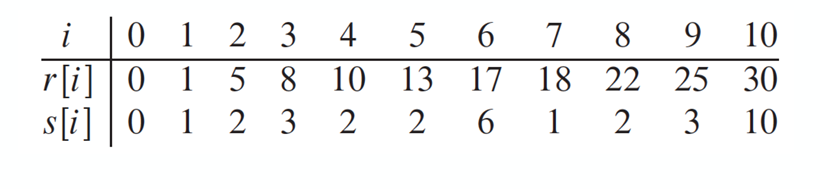
\includegraphics[width=1\linewidth]{immagini//capitolo 13/13_5.png}
    \caption{Result printed}
    \label{fig:enter-label}
\end{figure}

\section{Longest Common Subsequence (LCS)}

The Longest Common Subsequence (LCS) problem involves finding the longest subsequence that is common to two sequences \(x\) and \(y\), where a subsequence is a sequence derived from another sequence by deleting some elements without changing the order of the remaining elements.

\subsection{Problem Definition}
Given two sequences:
\begin{itemize}
    \item \(x = [a, b, c, b, d, a, b]\)
    \item \(y = [b, d, c, a, b, a]\)
\end{itemize}
Determine a longest common subsequence. For the example above, the LCS can be one of \(\{\text{bdab, bcab, bcba}\}\), each of length 4.

\subsection{Brute Force Algorithm}
A brute force approach checks every subsequence of \(x[1, \dots, m]\) to see if it is also a subsequence of \(y[1, \dots, n]\). \newline
\textbf{Analysis:}
\begin{itemize}
    \item Checking if a subsequence of \(x\) is a subsequence of \(y\) takes \(O(n)\), as it involves scanning \(y\).
    \item The number of subsequences of \(x\) is \(2^m\) because for each element I have two option: include it o don't include it.
    \item Therefore, the total cost is \(O(n \cdot 2^m)\).
\end{itemize}

\subsection{Simplification}
To simplify, we focus on the length of the LCS, \(c[x, y]\), which is unique. Using this, we can extend the algorithm to find one LCS. The strategy involves considering prefixes of \(x\) and \(y\), and expressing the length of their LCS in terms of smaller prefixes. \newline
\textbf{Definition:} \(c[i, j] = |\text{LCS}(x[1, \dots, i], y[1, \dots, j])|\)
\begin{itemize}
    \item \(c[i, j]\) is the length of the LCS for prefixes \(x[1, \dots, i]\) and \(y[1, \dots, j]\).
    \item Our goal is to compute \(c[m, n]\), the length of the LCS of \(x\) and \(y\). We want to express it in terms of other c[i,j] which we have previously calculate  $\forall i,j\in n,m$
\end{itemize}

\section{Proof of the Longest Common Subsequence (LCS) Algorithm}
\begin{align*}
    c[i, j] = \begin{cases}
        0, & \text{if } i = 0 \text{ or } j = 0, \\
        c[i-1, j-1] + 1, & \text{if } x[i] = y[j], \\
        \max\{c[i, j-1], c[i-1, j]\}, & \text{otherwise.}
    \end{cases}
\end{align*}

\subsection{Base Case}
\begin{itemize}
    \item \( c[i,j] = 0 \): This is true when one of the two sequences is empty because they have no elements in common.
\end{itemize}

\subsection{Case 1: \( x[i] = y[j] \)}
\begin{itemize}
    \item Assume there exists a common subsequence \( z[1,\dots,k] = \text{LCS}(x[1,\dots,i], y[1,\dots,j]) \) where \( c[i,j]=k \).
    \item Since \( x[i] = y[j] \), we can conclude that \( z[k] = x[i] = y[j] \). This is because if \( z \) does not include \( x[i] \) or \( y[j] \), then we could add this character to \( z \) to make it longer, contradicting the fact that \( z \) is the longest common subsequence (LCS).
    \item Hence, \( z[1,\dots,k-1] \) is a common subsequence (CS) of \( x[1,\dots,i-1] \) and \( y[1,\dots,j-1] \).
    \item \textbf{Claim}: \( z[1,\dots,k-1] \) is a \textit{longest} common subsequence (LCS) of \( x[1,\dots,i-1] \) and \( y[1,\dots,j-1] \).
\end{itemize}

\subsection{Proof of the Claim}
\begin{itemize}
    \item By contradiction, assume that \( w \) is a longer common subsequence than \( z \), such that \( |w| > k-1 \).
    \item Using a \textit{cut-and-paste argument}, concatenate \( w \) with \( z[k] \), forming \( w|z[k]| \).
    \item \( w|z[k]| \) is a common subsequence of \( x[1,\dots,i] \) and \( y[1,\dots,j] \) with a length greater than \( k \), which contradicts the assumption that \( z \) is the LCS.
    \item Therefore, \( c[i-1,j-1] = k-1 \), which implies \( c[i,j] = c[i-1,j-1] + 1 \).
\end{itemize}

\subsection{Case 2: \( x[i] \neq y[j] \)}
\begin{itemize}
    \item The proof for this case follows a similar reasoning and shows that:
    \[
    c[i,j] = \max(c[i-1,j], c[i,j-1])
    \]
\end{itemize}

\subsection{Optimal Substructure}
\begin{itemize}
    \item The problem exhibits \textit{optimal substructure}, meaning that the solution to the overall problem is composed of optimal solutions to its subproblems.
    \item If \( z = \text{LCS}(x, y) \), then any prefix of \( z \) is an LCS of a prefix of \( x \) and a prefix of \( y \).
\end{itemize}

\subsection{Recursive Algorithm}
\begin{verbatim}
LCS(x, y, i, j):
    # i, j are the last indices of x and y
    if i == 0 or j == 0:
        return 0  # Base case: one sequence is empty
    if x[i] == y[j]:
        return LCS(x, y, i-1, j-1) + 1  # Characters match
    else:
        return max(LCS(x, y, i-1, j), LCS(x, y, i, j-1))
\end{verbatim}

\textbf{Explanation of the Code:}
\begin{itemize}
    \item The function computes \(c[i, j]\) recursively based on the cases in the formula.
    \item Base cases handle when one sequence is empty.
    \item When \(x[i] = y[j]\), the LCS includes this character, and we compute the LCS for the remaining prefixes.
    \item When \(x[i] \neq y[j]\), the LCS is the maximum of excluding either \(x[i]\) or \(y[j]\).
\end{itemize}

\section{Worst Case Analysis for LCS}

The main computational challenge in the recursive LCS algorithm arises from the \texttt{else} clause, where two recursive calls are made. This creates an exponential growth in the number of subproblems solved. To illustrate, consider the case where $n=7$ and $m=6$. The recursion tree is as follows:

\begin{figure}[h!]
    \centering
    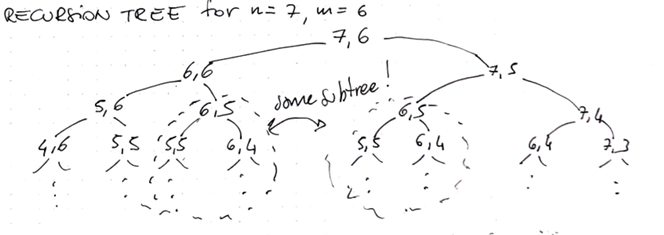
\includegraphics[width=1\linewidth]{immagini//capitolo 13/13_6.png}
    \label{fig:enter-label}
\end{figure}
As we observe, there are repeated subtrees, which indicate redundant computations. This redundancy can be eliminated using dynamic programming. The height of the recursion tree is $m+n$. Since it is a binary tree, each level introduces $2^i$ work, leading to a time complexity of $O(2^{m+n})$. However, LCS contains only $m \cdot n$ distinct subproblems. By storing the results of these subproblems, we avoid redundant computations. \newpage
The recurrence relation for the LCS problem is:
\[
T(n,m) = \begin{cases}
    T(n-1,m-1) + O(1), & \text{if } x[n] = y[m], \\
    T(n-1,m) + T(n,m-1) + O(1), & \text{otherwise}.
\end{cases}
\]
This exponential growth motivates the need for a bottom-up approach.

\subsection{Bottom-Up Memoized Algorithm}

The bottom-up approach systematically computes solutions for smaller subproblems first and uses them to construct the solution for larger subproblems. The pseudocode is as follows:

\begin{verbatim}
LCS-LENGTH(x, y, m, n)
    let b[1,...,m, 1,...,n] and c[0,...,m, 0,...,n] be new tables
    for i = 1 to m do
        c[i,0] = 0
    for j = 0 to n do
        c[0,j] = 0 #define the matrix c to zero
    for i = 1 to m do
        for j = 1 to n do
            if x[i] == y[j] then
                c[i,j] = c[i-1,j-1] + 1
                b[i,j] = " "  # northwest arrow
            else if c[i-1,j] >= c[i,j-1] then #if element up is >= than element left than
                c[i,j] = c[i-1,j] #copy from up
                b[i,j] = "↑"  # north arrow
            else
                c[i,j] = c[i,j-1] #copy from left
                b[i,j] = "←"  # west arrow
    return c, b
\end{verbatim}

\textbf{Explanation:}
\begin{itemize}
    \item The \texttt{c} table stores the lengths of LCS for prefixes of $x$ and $y$. b and c are matrixes.
    \item The \texttt{b} table stores arrows that indicate the direction of the optimal solution (northwest, north, or west).
    \item Base cases initialize the first row and column to 0, as an empty sequence has no common subsequence with any other sequence.
    \item This is a bottom up memoization algorithm because I start with the base case by setting the matrix element to 0 if i of j is equal to zero. In addition to that there isn't recursion.
\end{itemize}
\newpage
\subsection{Exercise}
Consider the sequences:
\begin{itemize}
    \item $x = A B C B D A B$
    \item $y = B D C A B A$
\end{itemize}

\begin{figure}[h!]
    \centering
    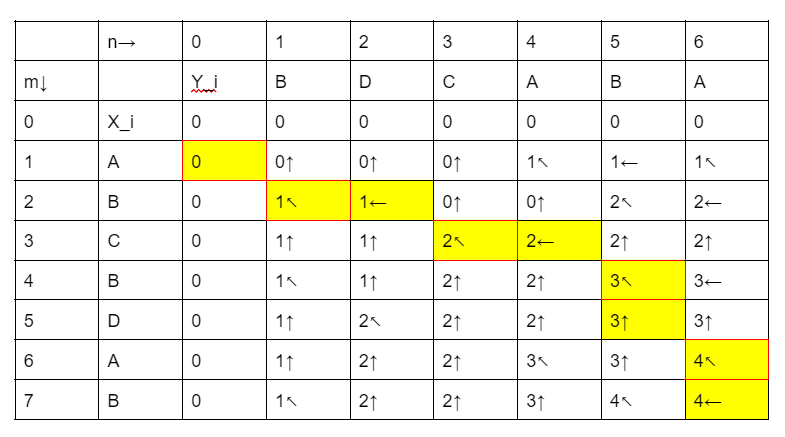
\includegraphics[width=1\linewidth]{immagini//capitolo 13/13_7.png}
    \label{fig:enter-label}
\end{figure}


\textbf{Instructions:}
\begin{itemize}
    \item If the characters at the current indexes match, copy the diagonal value and add 1.
    \item If they do not match, take the maximum value from the cell above or to the left. In case of a tie, prefer the top cell.
    \item Draw arrows in the \texttt{b} table to indicate the source of each value.
\end{itemize}

Starting from the bottom-right corner, trace back along the northwest arrows to construct the LCS and print a letter when you find the north-west arrow. Stop when a cell with value 0 is reached.

\subsection{Printing the LCS}

To print the LCS, we use the following recursive function:

\begin{verbatim}
PRINT-LCS(b, x, i, j)
    if i == 0 or j == 0
        return
    if b[i,j] == "↖ " then # north-west arrow 
        PRINT-LCS(b, x, i-1, j-1)
        print x[i]
    else if b[i,j] == "↑" then
        PRINT-LCS(b, x, i-1, j)  # Go up
    else
        PRINT-LCS(b, x, i, j-1)  # Go left
\end{verbatim}

\textbf{Explanation:}
\begin{itemize}
    \item The function recursively traverses the \texttt{b} table.
    \item It prints characters of $x$ only when a northwest arrow is encountered starting from bottom left.
    \item This ensures the correct order of characters in the LCS.
\end{itemize}

\section{Dynamic Programming: Text Justification}

\subsection{Problem Statement}
Given a sequence of words and a limit on the number of characters per line (\textit{line width}), we aim to insert line breaks in the sequence such that the lines are printed neatly.
\begin{figure}[h!]
    \centering
    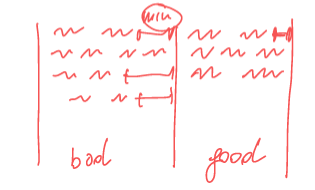
\includegraphics[width=0.75\linewidth]{immagini//capitolo 13/13_8.png}
    \label{fig:enter-label}
\end{figure}
\paragraph{Input:} An array of words $l = w[0, \ldots, n-1]$, where $|l| = n$.

\paragraph{Scoring Rule:} 
Suppose we consider the words from index $i$ to $j$ ($w[i], w[i+1], \ldots, w[j]$). We define the \textbf{badness} of this justification as:
\[
\text{badness}(i, j) =
\begin{cases}
+\infty & \text{if } j+1-i > \text{page\_width}, \\
\big(\text{page\_width} - (len(w[i]+ w[i+1]+\ldots+w[j] + 1)\big)^2 & \text{otherwise.}
\end{cases}
\]
Our goal is to divide the words in order to minimize the total badness.

\subsection{Brute-Force Algorithm}
A naive algorithm examines all possible ways to divide the sequence into lines. This approach has a complexity of $\mathcal{O}(2^n)$, which is impractical for large inputs.

\subsection{Dynamic Programming Approach}
We can reduce the complexity by leveraging the structure of the problem.

\paragraph{Subproblems:} 
Define the cost $c[i]$ as the minimum badness of dividing the suffix $w[i, \ldots, n-1]$ into lines:
\[
c[i] = \min\big(\text{badness}(i, j) + c[j+1]\big) \quad \text{for all } j \in [i, n-1].
\]
Here:
\begin{itemize}
    \item Computing $\text{badness}(i, j)$ requires $\mathcal{O}(1)$ operations.
    \item The recurrence considers up to $n-i+1$ choices for $j$, so each $c[i]$ computation is $\mathcal{O}(n)$.
\end{itemize}
Thus, the overall complexity is $\mathcal{O}(n^2)$.

\subsection{Example}
Suppose we have the following \textbf{Words:} ``diamonds are girl's best friends'' and a
\textbf{Page Width} equal to 12.

\paragraph{Word Table:}
\[
\begin{array}{|c|c|c|}
\hline
i & \text{Word} & \text{Length} \\
\hline
0 & \text{diamonds} & 8 \\
1 & \text{are} & 3 \\
2 & \text{girls} & 5 \\
3 & \text{best} & 4 \\
4 & \text{friends} & 7 \\
\hline
\end{array}
\]

\paragraph{Greedy Approach:}
In this approach, we fill each line as much as possible before moving to the next line. The resulting layout and badness are as follows:

\[
\begin{array}{|c|c|}
\hline
\text{Line} & \text{Badness} \\
\hline
\text{diamonds are} & 0 \\
\text{girls best} & 2^2 \\
\text{friends} & 5^2 \\
\hline
\text{Total Badness} & 29 \\
\hline
\end{array}
\]

\paragraph{Dynamic Programming Approach:}
The dynamic programming solution minimizes the total badness. The resulting layout and badness are as follows:

\[
\begin{array}{|c|c|}
\hline
\text{Line} & \text{Badness} \\
\hline
\text{diamonds} & 4^2 \\
\text{are girls} & 3^2 \\
\text{best friends} & 0 \\
\hline
\text{Total Badness} & 25 \\
\hline
\end{array}
\]
In the DP approach, we compute the badness of all possible divisions and store intermediate results to avoid recomputation. This results in a more optimal layout than the greedy approach.

\subsection{Optimal Solution}
To find the best way to justify the text, we calculate the \textbf{badness matrix}, which stores the cost of fitting words from index $i$ to $j$ on one line. The process involves two main steps:
\begin{enumerate}
    \item Compute the badness for each possible grouping of words.
    \item Use dynamic programming to find the minimum cost and reconstruct the optimal solution.
\end{enumerate}

\paragraph{Badness Matrix Table:}
\[
\begin{array}{|c|c|c|c|c|c|}
\hline
i \downarrow \backslash j \rightarrow & 0 \, (\text{diamonds}) & 1 \, (\text{are}) & 2 \, (\text{girls}) & 3 \, (\text{best}) & 4 \, (\text{friends}) \\
\hline
0 & 16 & 0 & \infty & \infty & \infty \\
1 & - & 81 & 9 & \infty & \infty \\
2 & - & - & 49 & 4 & \infty \\
3 & - & - & - & 64 & 0 \\
4 & - & - & - & - & 25 \\
\hline
\end{array}
\]
The matrix is half-empty because it represents only valid groupings of words.

\paragraph{Dynamic Programming Arrays:}
We define two arrays:
\begin{itemize}
    \item \textbf{minCost:} Stores the minimum cost for justifying the suffix starting at word $i$.
    \item \textbf{index:} Stores the index used to reconstruct the optimal solution.
\end{itemize}

\subsection{Step-by-Step Computation}
\begin{figure}[h!]
    \centering
    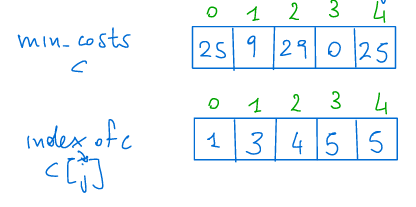
\includegraphics[width=1\linewidth]{immagini//capitolo 13/13_9.png}
    \label{fig:enter-label}
\end{figure}


\begin{itemize}
    \item \textbf{First Iteration:} By default we start from the last word (\textit{friends}), we set the last element of minCost with the value of the badness(n-1,n-1) e index[n-1] = n, where n is the number of words. Therefore $minCost[4] = 25$ and $index[4] = 5$. 
    \item \textbf{Second Iteration:} From now on, we compute for each $i$ from $n-2$ to 0 the quantity $\text{badness}(i,j) + \text{minCost}[j+1]$ for all $j \in (i, n-1)$ and select the minimum. This will be $\text{minCost}[i]$, and we set $\text{index}[i] = j+1$ where $j$ is the index used to obtain $\text{minCost}[i]$. In our calculations, we may encounter cases where we compute $\text{minCost}[j^*]$ where $j^* > n-1$; in this case, set $\text{minCost}[j^*] = 0$. \newline
    Now i = n-2=3 and j$\in (3,4)$. We compute:
    \begin{align*}
         &\text{badness}(3,3) + minCost[4] = 64 + 25 = 89 \\
         &\text{badness}(3,4) + minCost[5] = 0 + 0   = 0
    \end{align*}
    We set minCost[3] = 0 and index[3] = 5. 
    \item \textbf{Third Iteration:} Now i = 2 and j$\in (2,3,4)$. We compute:
    \begin{align*}
        &\text{badness}(2,2) + minCost[3] = 49 + 0 = 49 \\
        &\text{badness}(2,3) + minCost[4] = 4 + 25 = 29 \\
        &\text{badness}(2,4) + minCost[5] = \infty + 0 = \infty
    \end{align*}
    We set minCost[2] = 29 and index[2] = 4. 
    \item \textbf{Fourth Iteration:} Now i = 1 and j$\in (1,2,3,4)$. We compute:
    \begin{align*}
        &\text{badness}(1,1) + minCost[2] = 81 + 29 = 110 \\
        &\text{badness}(1,2) + minCost[3] = 9 + 0 = 9 \\
        &\text{badness}(1,3) + minCost[4] = \infty + 25= \infty \\
        &\text{badness}(1,4) + minCost[5] = \infty + 0 = \infty
    \end{align*}
    We set minCost[1] = 9 and index[1] = 3. 
    \item \textbf{Fifth Iteration:} Now i = 0 and j$\in (0,1,2,3,4)$. We compute:
    \begin{align*}
        &\text{badness}(0,0) + minCost[1] = 16 + 9 = 25 \\
        &\text{badness}(0,1) + minCost[2] = 0 + 29 = 29 \\
        &\text{badness}(0,2) + minCost[3] = \infty + 0 = \infty \\
        &\text{badness}(0,3) + minCost[4] = \infty + 25= \infty \\
        &\text{badness}(0,4) + minCost[5] = \infty + 0 = \infty
    \end{align*}
    We set minCost[0] = 25 and index[0] = 1.
\end{itemize}

\paragraph{Optimal Layout:}
To print the words, we look at the first element of the $\text{index}$ vector. This indicates the index up to which we can print the words. For example, if the element $\text{index}[0]$ is 1, it means that we can print the words up to word 1 excluded, therefore only word 0, which is "diamond", and then go to a new line. To understand how many words to place on the second line, we use the element that was in the previously examined position, i.e., 1, as the index of the vector. $\text{index}[1] = 3$, so we can print words 1 and 2, which are "are girls". We apply this procedure again and obtain that in the third line we can put the words up to number $\text{index}[3] = 5$, therefore words 3 and 4. If we had had other words, we could have continued.
\paragraph{Optimal Justification:}
\begin{verbatim}
diamonds
are girls
best friends
\end{verbatim}

\subsection{Pseudocode}
\textbf{Main Algorithm:}
\begin{verbatim}
TEXT-JUSTIFICATION(W, page_width)
input: an array of words W and page_width
output: minimum Cost and list of indexes for optimal justification

// Initialize the badness matrix
let badness[0 .. len(W)-1, 0 .. len(W)-1] be empty
for i <- 0 to len(W)-1 do
    badness[i,i] <- page_width - len(W[i])
    for j <- i+1 to len(W)-1 do
        badness[i,j] <- badness[i,j-1] - len(W[j]) - 1

// Compute badness values
for i <- 0 to len(W)-1 do
    for j <- i to len(W)-1 do
        if badness[i,j] < 0 then
            badness[i,j] <- infinity
        else:
            badness[i,j] <- badness[i,j]^2

// Calculate minCost and index arrays
let minCost[0 .. len(W)-1], index[0 .. len(W)-1] be empty
for i <- len(W)-1 to 0 do
    minCost[i] <- badness[i, len(W)-1]
    index[i] <- len(W)-1
    for j <- len(W)-1 to i+1 do
        if badness[i,j-1] != infinity and minCost[i] > badness[i,j-1] + minCost[j] then
            minCost[i] <- badness[i,j-1] + minCost[j]
            index[i] <- j
return (minCost, index)
\end{verbatim}

\textbf{Text Printing Algorithm:}
\begin{verbatim}
PRINT-JUSTIFIED-TEXT(W, page_width)
(minCost, index) <- TEXT-JUSTIFICATION(W, page_width)
i <- 0
do:
    j <- index[i]
    for k <- i to j-1 do:
        if k != j-1 then
            print(W[k] + " ") // Add space for all but last word
        else:
            print(W[k]) // Print last word in the line
    print("\n") // Move to the next line
    i <- j
while i < len(W)
\end{verbatim}

\section{All Pairs Shortest Path Problem}
The \textbf{All Pairs Shortest Path (APSP)} problem involves finding the shortest path between every pair of vertices in a graph \( G = (V, E) \). 

The \textbf{Floyd-Warshall Algorithm} solves the APSP problem in \( \Theta(V^3) \) time, which is efficient for dense graphs. This algorithm:
\begin{itemize}
    \item Works with directed graphs with weighted edges.
    \item Handles negative weights but requires that there are no negative weight cycles.
    \item Considers intermediate vertices in paths.
\end{itemize}

\subsection{Intermediate Vertices and Paths}
To compute the shortest path, the algorithm considers intermediate vertices in a path. Let:
\[
p = \langle v_1, v_2, \dots, v_l \rangle
\]
represent a path, where intermediate vertices are:
\[
\{v_2, v_3, \dots, v_{l-1}\}.
\]

\subsection{Key Lemma}
\textbf{Lemma 1:}  
Given a weighted directed graph \( G = (V, E) \) with \( w: E \to \mathcal{R} \), let:
\[
p = \langle v_0, v_1, \dots, v_k \rangle
\]
be the \textbf{Shortest Path (SP)} from \( v_0 \) to \( v_k \). For any \( i, j \) such that \( 0 \leq i \leq j \leq k \), the subpath:
\[
p_{ij} = \langle v_i, v_{i+1}, \dots, v_j \rangle
\]
is the shortest path from \( v_i \) to \( v_j \).

\textbf{Proof:}  
If a shorter path \( p'_{ij} \) exists, \( p \) would no longer be the shortest path. Thus, \( p_{ij} \) must also be the shortest path.

\subsection{Intermediate Nodes in Shortest Paths}

Given \( V = \{v_1, v_2, \dots, v_n\} \), consider a subset \( \{v_1, v_2, \dots, v_k\} \) for some \( k < n \). For any \( i, j \in V \), consider all paths from \( i \) to \( j \) whose intermediate vertices are drawn from \( \{v_1, \dots, v_k\} \), and let \( p \) be the shortest path (SP) among them.

Now consider the subset \( \{v_1, v_2, \dots, v_{k-1}\} \):
\begin{itemize}
    \item If \( k \) is \textbf{not an intermediate node of \( p \)}, then all intermediate nodes of \( p \) are in \( \{v_1, v_2, \dots, v_{k-1}\} \). In this case, the SP from \( i \) to \( j \) with intermediates in \( \{v_1, v_2, \dots, v_{k-1}\} \) is also the SP with intermediates in \( \{v_1, v_2, \dots, v_k\} \).

    \item If \( k \) \textbf{is an intermediate node of \( p \)}, then the path can be expressed as \( p = i \to k \to j \). Here, \( p_1 = i \to k \) and \( p_2 = k \to j \) are subpaths of \( p \). By Lemma 1, \( p_1 \) is the SP from \( i \) to \( k \) with intermediates in \( \{v_1, \dots, v_k\} \), and \( p_2 \) is the SP from \( k \) to \( j \) with intermediates in \( \{v_1, \dots, v_k\} \).
\end{itemize}

This observation leads directly to the recurrence relation that will be used to compute the shortest paths incrementally as we consider more intermediate nodes.

\subsection{Recursive Solution}
Let \( d^{(k)}_{ij} \) represent the weight of the shortest path from \( i \) to \( j \) using only the vertices \( \{v_1, v_2, \dots, v_k\} \) as intermediate vertices.

\paragraph{Base Case (\( k = 0 \)):}
\[
d^{(0)}_{ij} = 
\begin{cases} 
w(i, j), & \text{if } (i, j) \in E, \\
0, & \text{if } i = j, \\
\infty, & \text{otherwise.}
\end{cases}
\]

\paragraph{Recursive Step (\( k \geq 1 \)):}
\[
d^{(k)}_{ij} = 
\min\big(d^{(k-1)}_{ij}, d^{(k-1)}_{iK} + d^{(k-1)}_{Kj}\big).
\]

Here:
\begin{itemize}
    \item \( d^{(k-1)}_{ij} \): The shortest path without using vertex \( k \) as an intermediate.
    \item \( d^{(k-1)}_{iK} + d^{(k-1)}_{Kj} \): The path through vertex \( k \).
\end{itemize}

\paragraph{Final Answer:}  
The matrix \( D^{(n)} \) gives \( d^{(n)}_{ij} = \delta(i, j) \) for all \( i, j \in V \).

\subsection{Algorithm Description}
The input is a weight matrix \( W \) where:
\[
w_{ij} = 
\begin{cases} 
0, & \text{if } i = j, \\
w(i, j), & \text{if } (i, j) \in E, \\
\infty, & \text{otherwise.}
\end{cases}
\]
The output is a matrix \( D^{(n)} \) containing shortest path distances. \newline
\textbf{Pseudocode:}
\begin{verbatim}
FLOYD-WARSHALL(W)
    n = rows[W]
    D^(0) <- W
    for k = 1 to n do
        for i = 1 to n do
            for j = 1 to n do
                D^(k)[i][j] = min(D^(k-1)[i][j], 
                                  D^(k-1)[i][k] + D^(k-1)[k][j])
    return D^(n)
\end{verbatim}

\paragraph{Explanation:}
\begin{itemize}
    \item \( D^{(0)} \): Initialize using the weight matrix \( W \).
    \item For each intermediate vertex \( k \), update the distance matrix \( D \) by considering paths through \( k \).
    \item The algorithm iterates over all \( i, j \) pairs for each \( k \), resulting in a cubic complexity \( \Theta(V^3) \).
\end{itemize}

\subsection{Complexity Analysis}
The Floyd-Warshall Algorithm has a time complexity of:
\[\Theta(V^3)\] which is efficient for dense graphs. It computes the shortest paths for all vertex pairs in \( V \), making it a versatile algorithm for graph analysis.

\section{Purpose of the \( \Pi \)-Matrix in Floyd-Warshall Algorithm}

The \( \Pi \)-matrix (or predecessor matrix) is used in the Floyd-Warshall algorithm to reconstruct the shortest paths between all pairs of vertices. While the \( D \)-matrix stores the minimum distances, the \( \Pi \)-matrix tracks the predecessors in the shortest paths.

\subsection{Role of the \( \Pi \)-Matrix}
\begin{itemize}
    \item \textbf{Path Reconstruction:}
    The entry \( \Pi[i][j] \) represents the vertex immediately before \( j \) in the shortest path from \( i \) to \( j \). By following the predecessor chain in the \( \Pi \)-matrix, it is possible to reconstruct the shortest path.

    \item \textbf{Initialization:}
    \begin{itemize}
        \item If there is an edge from \( i \) to \( j \), \( \Pi[i][j] \) is initialized to \( i \) because \( i \) is the predecessor of \( j \).
        \item If there is no direct edge between \( i \) and \( j \), \( \Pi[i][j] \) is initialized to \( \text{None} \) or \( -1 \) to indicate that no path exists initially.
    \end{itemize}

    \item \textbf{Update Rule:}
    During the algorithm's execution, whenever a shorter path from \( i \) to \( j \) through \( k \) is found, \( \Pi[i][j] \) is updated to reflect the new predecessor:
    \[
    \Pi[i][j] = \Pi[k][j]
    \]
\end{itemize}

\subsection{Example of Use}
Suppose the following \( \Pi \)-matrix is obtained after running the Floyd-Warshall algorithm:
\[
\Pi = 
\begin{bmatrix}
- & 1 & 1 & 2 \\
2 & - & 2 & 2 \\
3 & 3 & - & 3 \\
4 & 4 & 4 & -
\end{bmatrix}
\]

To find the shortest path from vertex \( 1 \) to \( 4 \):
\begin{enumerate}
    \item Start at vertex \( 4 \) (the destination).
    \item Look at \( \Pi[1][4] = 2 \), which means the predecessor of \( 4 \) in the shortest path is \( 2 \).
    \item Now look at \( \Pi[1][2] = 1 \), which means the predecessor of \( 2 \) in the shortest path is \( 1 \).
    \item Thus, the shortest path is \( 1 \to 2 \to 4 \).
\end{enumerate}

\subsection{Benefits}
The \( \Pi \)-matrix provides the following advantages:
\begin{itemize}
    \item It complements the \( D \)-matrix: while \( D \) gives the shortest distances, \( \Pi \) enables the reconstruction of the actual paths.
    \item It avoids recomputing the path dynamically by storing the predecessor information during the algorithm execution.
\end{itemize}

\subsection{Summary}
The \( \Pi \)-matrix ensures that the Floyd-Warshall algorithm not only computes the shortest distances but also provides a way to determine the actual sequence of vertices in each shortest path. This is particularly useful in applications requiring explicit paths, such as navigation systems or route planning.


\section{Floyd-Warshall Algorithm: Example and Solution}

\subsection{Problem Description}
We are given a directed weighted graph \( G = (V, E) \) with the following edges and weights:
\begin{itemize}
    \item \( 1 \to 2 \): Weight = 3
    \item \( 1 \to 5 \): Weight = -4
    \item \( 2 \to 3 \): Weight = 4
    \item \( 2 \to 5 \): Weight = 7
    \item \( 3 \to 4 \): Weight = -5
    \item \( 4 \to 2 \): Weight = 1
    \item \( 5 \to 4 \): Weight = 6
\end{itemize}
The goal is to compute the shortest paths between all pairs of vertices using the Floyd-Warshall algorithm.

\subsection{Graph Representation}
The graph can be represented as follows:

\subsection{Algorithm Description}
The Floyd-Warshall algorithm computes the shortest path between all pairs of vertices by iteratively considering intermediate vertices. The key recurrence relation is:
\[
d^{(k)}_{ij} = \min\big(d^{(k-1)}_{ij}, d^{(k-1)}_{iK} + d^{(k-1)}_{Kj}\big),
\]
where \( d^{(k)}_{ij} \) represents the shortest path from vertex \( i \) to vertex \( j \), considering the first \( k \) vertices as potential intermediates.

\subsection{Initialization}
The initial distance matrix \( D^{(0)} \) and predecessor matrix \( \Pi^{(0)} \) are defined as follows:

\subsection{Conclusion}
After all iterations, the final \( D^{(n)} \) matrix contains the shortest path distances between all pairs of vertices, and the \( \Pi^{(n)} \) matrix contains the predecessors for reconstructing the paths.
\begin{figure}[h!]
    \centering
    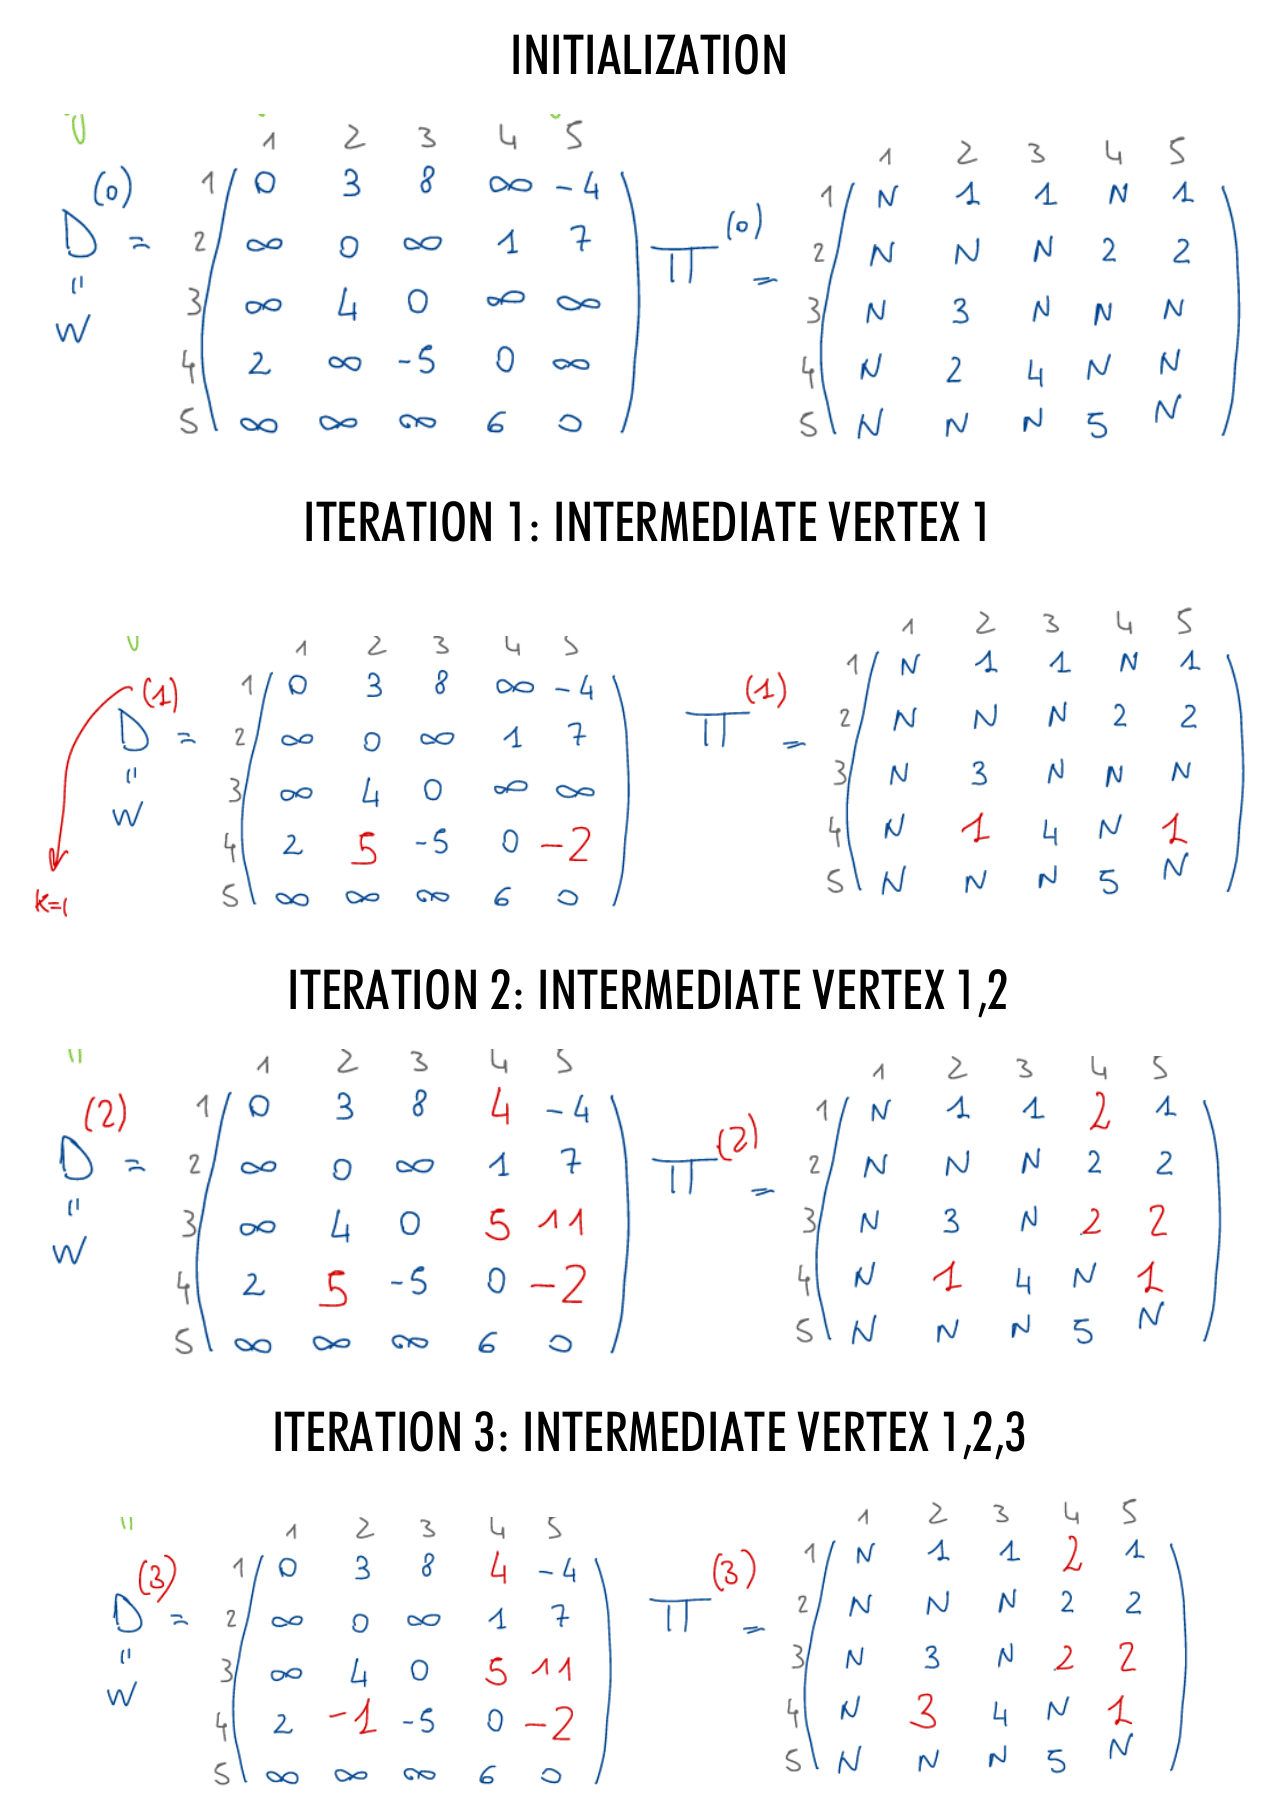
\includegraphics[width=0.7\linewidth]{immagini//capitolo 14 esercizio/INITIALIZATION-1.png}
    \caption{Enter Caption}
    \label{fig:enter-label}
\end{figure}

\newpage
\begin{figure}[h!]
    \centering
    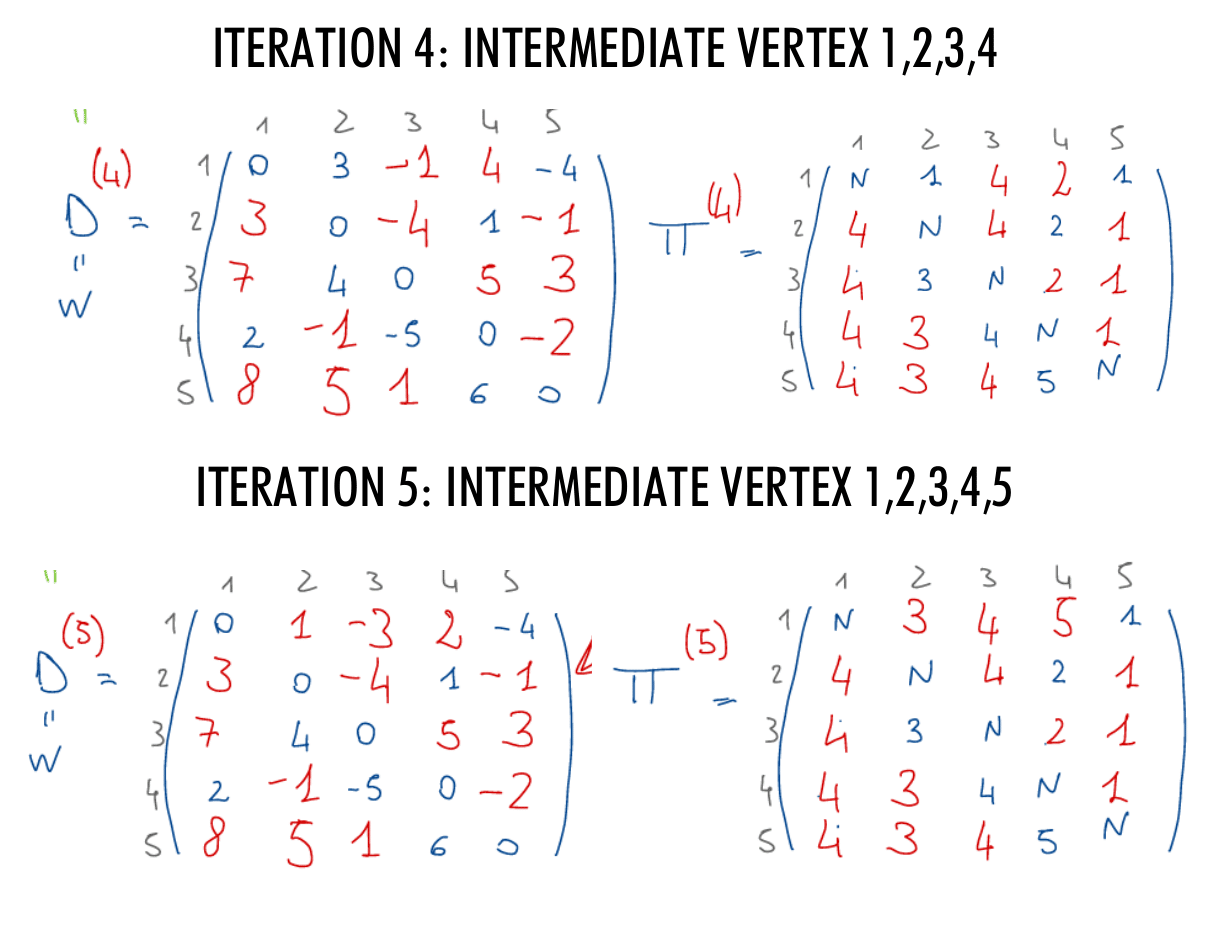
\includegraphics[width=0.75\linewidth]{immagini//capitolo 14 esercizio/INITIALIZATION-2.png}
    \caption{Enter Caption}
    \label{fig:enter-label}
\end{figure}

\begin{figure}[h!]
    \centering
    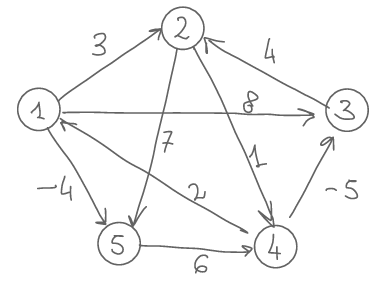
\includegraphics[width=0.75\linewidth]{immagini//capitolo 14 esercizio/14_grafo.png}
\end{figure}




\chapter{Basic Graph Algorithm}

\section{Outline}
In this document, we will explore some fundamental algorithms and representations used in graph theory. We will cover the following topics:
\begin{itemize}
    \item How to represent graphs (Graph Representation)
    \item Breadth-First Search (BFS), a method for exploring graphs layer by layer
    \item Depth-First Search (DFS), which dives deeply into one branch before backtracking
    \item Directed Acyclic Graphs (DAGs), a special kind of directed graph with no cycles
\end{itemize}

\section{Graph Basics}
A graph is a structure that consists of two main components:
\begin{itemize}
    \item A set of vertices $V$ (also called nodes)
    \item A set of edges $E$, which connect pairs of vertices
\end{itemize}

Graphs can be used to model a wide range of real-world problems, from social networks to transportation systems. Let's break down some of the different types of graphs you might encounter.

\subsection{Types of Graphs}
Graphs can vary greatly in their structure and properties. Here are some important types:
\begin{itemize}
    \item \textbf{Undirected Graphs:} In an undirected graph, edges have no direction. This means if there is an edge between vertices $u$ and $v$, you can travel from $u$ to $v$ and vice versa. Formally, $(u, v) = (v, u)$. Self-loops (e.g. (v,v)) are not allowed.
    \item \textbf{Directed Graphs:} In directed graphs, edges have a specific direction. If there is an edge from $u$ to $v$, you cannot travel back from $v$ to $u$ unless a separate edge exists. This is written as $u \to v$. Self-loops are allowed.
    \item \textbf{Weighted Graphs:} In weighted graphs, each edge carries a value or cost, often representing distance or time. A weight function $w : E \to \mathbb{R}$ assigns a real number to each edge.
    \item \textbf{Dense and Sparse Graphs:} A graph is dense if it has a large number of edges, close to $|V|^2$. Conversely, a sparse graph has far fewer edges, often closer to $|V|$. $|E|$ = O($|V|^2$)
    \item \textbf{Connected Graphs:} A graph is \textbf{connected} if there is a path between every pair of vertices. In simpler terms, you can get from any vertex to any other vertex by following a series of edges. For a connected graph, the number of edges is at least $|V| - 1$. If the graph has exactly $|V| - 1$ edges and is connected, it forms a special structure called a tree.
\end{itemize}
When two vertices are connected by an edge, we say they are \textit{adjacent}. This relationship is symmetric in undirected graphs but not necessarily so in directed graphs.



\section{Graph Representation}
There are two main ways to represent graphs in computer programs: adjacency lists and adjacency matrices.

\begin{figure}[h]
    \centering
    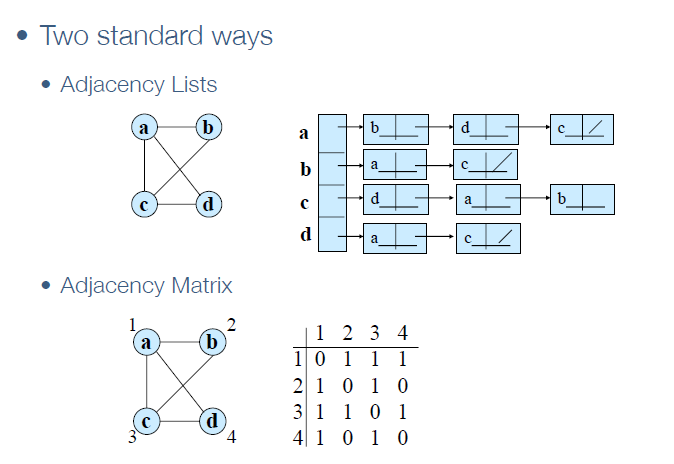
\includegraphics[width=0.75\linewidth]{graph representation.png}

\end{figure}

\subsection{Adjacency List Representation}
\begin{figure}[h!]
    \centering
    \includegraphics[width=0.75\linewidth]{adjacency list representation.png}

\end{figure}
Adjacency lists provide an efficient way to store graphs, especially when the graph is sparse. Here's how it works:
\begin{itemize}
    \item We maintain an array of lists, one for each vertex.
    \item Each list contains all the vertices adjacent to that vertex ( e.g. For u $\in V$, Adj[u] consists of all vertices adjacent to u).
    \item For directed graphs, the sum of the lengths of all adjacency lists equals the number of edges $|E|$. For undirected graphs, the sum is $2|E|$ because each edge appears in two lists.
    \item The storage requirement for adjacency lists is $\Theta(|V| + |E|)$.
\end{itemize}
This representation is space-efficient when the graph is sparse and has few edges relative to the number of vertices. \newline
The Cons of Adjacency Lists are:
\begin{itemize}
    \item Determining if an edge $(u,v) \in G$ is not efficient
    \item Have to search in u’s adjacency list. $\Theta(degree(u))$ time, $\Theta(V)$ in the worst case.
\end{itemize}

\subsection{Adjacency Matrix Representation}
An adjacency matrix is a more straightforward, but often less efficient, way to represent graphs:
\begin{itemize}
    \item We use a $|V| \times |V|$ matrix $A$.
        \[
        A[i, j] = 
        \begin{cases}
            1 & \text{if (i,j)$\in$ E} \\
            0 & \text{otherwise } 
        \end{cases}
        \]
    \item If there is an edge between vertices $i$ and $j$, then $A[i, j] = 1$. Otherwise, $A[i, j] = 0$.
    \item The matrix requires \textbf{ $\Theta(V^2)$ space}, which can be wasteful for large graphs with few edges.
    \item However, checking if an edge exists between two vertices takes constant time, $\Theta(1)$.
\end{itemize}
\begin{figure}[h!]
    \centering
    \includegraphics[width=0.75\linewidth]{Adjacency matrix.png}[h]

\end{figure}

\section{Graph Nomenclature}
Let's go over some basic terminology that will help when working with graphs:
\begin{itemize}
    \item A \textbf{path} of length $k$ from vertex $u$ to vertex $v$ in a graph=$G=(V,E)$ is a sequence of edges $p=<u,u1,u2, … , v> $ where $(u,u1)$, $(u1,u2)$ and
so on belongs to E; $|p|$ = k.
    \item Vertex $v$ is \textbf{reachable} from $u$ if there exists a path connecting them.
    \item A path is \textbf{simple} if no vertex is repeated.
    \item A graph is \textbf{strongly connected} if there is a path between every pair of vertices in both directions.
\end{itemize}
\section{Graph Search Algorithms}
\subsection{Breadth-First Search (BFS)}
Breadth-First Search (BFS) is one of the most fundamental graph traversal algorithms. It explores a graph layer by layer, starting from a specified source vertex $s\in V$.

\textbf{How BFS Works:}
\begin{itemize}
    \item We begin at vertex $s$ and mark it as discovered.
    \item All vertices directly connected to $s$ are discovered next.
    \item We continue exploring vertices one layer at a time until all reachable vertices are visited.
    \item BFS builds a tree rooted at $s$ that includes all reachable vertices.
\end{itemize}

\textbf{Key Outputs:}
\begin{itemize}
    \item $d[v]$: The shortest distance (in terms of the number of edges) from $s$ to $v$. If $v$ is not reachable from $s$, $d[v] = \infty$.
    \item $\pi[v]$: The predecessor of $v$ on the shortest path from $s$.
\end{itemize}

To keep track of progress during the search, vertices are colored:
\begin{itemize}
    \item White: Undiscovered
    \item Gray: Discovered but not finished
    \item Black: Finished
\end{itemize}
\begin{figure}[h]
    \centering
\includegraphics[width=0.75\linewidth]{Breadth-Firs-Search.png}

\end{figure}
BFS is useful for finding the shortest path in unweighted graphs and discovering the overall structure of a graph.

\newpage
\section{Breadth-First and Depth-First Search}

\textbf{Breadth-First Tree}
When performing a Breadth-First Search (BFS) on a graph $G = (V, E)$ starting from a source vertex $s$, we can construct a subgraph known as the \textbf{Breadth-First Tree}. This subgraph provides valuable insights into the shortest paths from $s$ to other vertices.

\subsection{Definition}
The predecessor subgraph $G_\pi$ of $G$ is defined as:
\begin{itemize}
    \item $V_\pi = \{v \in V : \pi[v] \neq \text{NIL}\} \cup \{s\}$
    \item $E_\pi = \{(\pi[v], v) \in E : v \in V_\pi - \{s\} \}$
\end{itemize}
In simpler terms:
\begin{itemize}
    \item $V_\pi$ contains all vertices reachable from $s$.
    \item $E_\pi$ contains edges that link each vertex to its predecessor.
\end{itemize}
The predecessor subgraph $G_\pi$ forms a Breadth-First Tree if:
\begin{itemize}
    \item $V_\pi$ consists of vertices reachable from $s$.
    \item For each $v \in V_\pi$, there exists a unique simple path from $s$ to $v$, which is also the shortest path in $G$.
\end{itemize}
The edges in $E_\pi$ are referred to as \textbf{tree edges}, and the tree will have $|E_\pi| = |V_\pi| - 1$ edges.

\section{BFS Algorithm and Analysis}
\subsection{BFS Pseudocode}
\textbf{BFS(G, s)}
\begin{figure}[h]
    \centering
\includegraphics[width=1\linewidth]{BFS Pseudo code.png}

\end{figure}

\subsection{Analysis of BFS}
The BFS algorithm ensures that each vertex is enqueued and dequeued at most once. This results in a time complexity of $O(V)$ for queue operations. Additionally:
\begin{itemize}
    \item The adjacency list of each vertex is scanned at most once.
    \item Summing the lengths of all adjacency lists results in $O(E)$ operations.
    \item With the BFS method, we visit a number equal to the number of predecessors that discovered it, which corresponds to the in-degree.
\end{itemize}
Thus, the total running time of BFS is $O(V + E)$, which is linear with respect to the size of the graph.

\subsection{BFS:Example:}
\begin{figure}[h!]
    \centering
\includegraphics[width=0.75\linewidth]{BFS Ex. 1.png}
\end{figure}
\begin{figure} [h!]
    \centering
\includegraphics[width=0.75\linewidth]{BFS EX. 2.png}
\end{figure}
\newpage
\section{Depth-First Search (DFS)}

Depth-First Search (DFS) is a fundamental graph traversal algorithm used to explore all vertices and edges of a graph. The algorithm delves as deeply as possible along each branch before backtracking. It is particularly useful for tasks such as cycle detection, topological sorting, and connected component identification.

\subsection{Algorithm Overview}
The DFS algorithm explores edges out of the most recently discovered vertex \(v\). When all edges of \(v\) have been explored, it backtracks to the vertex from which \(v\) was discovered, continuing the process. This strategy embodies the principle: \emph{``Search as deep as possible first.''}

The process continues until all vertices reachable from the original source have been visited. If any undiscovered vertices remain, one of them is chosen as a new source, and the search is repeated.

\subsection{Input and Output}
\begin{itemize}
    \item \textbf{Input:} A graph \(G = (V, E)\), which can be directed or undirected. Unlike Breadth-First Search (BFS), no source vertex is specified initially.
    \item \textbf{Output:} 
    \begin{itemize}
        \item Two timestamps for each vertex:
        \begin{itemize}
            \item \(d[v]\): Discovery time, when \(v\) is first visited (color changes from white to gray).
            \item \(f[v]\): Finishing time, when the exploration of \(v\) is complete (color changes from gray to black).
        \end{itemize}
        \item \(\pi[v]\): Predecessor of vertex \(v\). For each vertex \(v\), \(\pi[v] = u\), where \(u\) is the vertex from which \(v\) was discovered.
    \end{itemize}
\end{itemize}

\subsection{Coloring Scheme}
DFS uses a coloring scheme to track the state of each vertex:
\begin{itemize}
    \item \textbf{White:} Vertex has not been discovered.
    \item \textbf{Gray:} Vertex has been discovered but is not yet fully explored.
    \item \textbf{Black:} Vertex and all its adjacent vertices have been fully explored.
\end{itemize}

\subsection{Key Steps of DFS}
\begin{enumerate}
    \item Initialize all vertices as white (unvisited), with \(\pi[v] = \text{NIL}\) and no timestamps.
    \item Start from an arbitrary vertex and mark it gray, recording its discovery time.
    \item Explore each unvisited adjacent vertex recursively.
    \item When all adjacent vertices of a vertex have been visited, mark it black and record its finishing time.
    \item Repeat the process for any remaining white vertices.
\end{enumerate}

\subsection{Applications of DFS}
DFS serves as the foundation for several advanced graph algorithms, including:
\begin{itemize}
    \item \textbf{Cycle detection:} Identifying cycles in directed or undirected graphs.
    \item \textbf{Topological sorting:} Ordering vertices in a Directed Acyclic Graph (DAG).
    \item \textbf{Connected components:} Finding connected subgraphs in an undirected graph.
    \item \textbf{Pathfinding:} Identifying paths between specific vertices.
\end{itemize}

\subsection{DFS Pseudocode}
The following pseudocode outlines the DFS algorithm:
\begin{verbatim}
DFS(G):
    for each vertex u in V[G]:
        color[u] ← white
        π[u] ← NIL
    time ← 0
    for each vertex u in V[G]:
        if color[u] == white:
            DFS-Visit(u)

DFS-Visit(u):
    color[u] ← gray
    time ← time + 1
    d[u] ← time
    for each v in Adj[u]:
        if color[v] == white:
            \pi[v] ← u
            DFS-Visit(v)
    color[u] ← black
    f[u] ← time
    time ← time + 1
\end{verbatim}

\subsection{Time Complexity}
The DFS algorithm operates in \(O(V + E)\) time for a graph \(G = (V, E)\) represented as an adjacency list. This efficiency arises because:
\begin{itemize}
    \item Each vertex is visited exactly once.
    \item Each edge is traversed at most twice (once for each vertex it connects).
\end{itemize}

\subsection{Classification of edges}
\begin{itemize}
    \item Tree edge: in the depth-first forest. Found by exploring (u, v). 
    \item Back edge: (u, v), where u is a descendant of v (in the depth-first tree). From v we can arrive to u. It is a back edge if the node is part of the tree and the edge leads to another node that is its ancestor.
    \item  Forward edge: (u, v), where v is a descendant of u, but not a tree edge. From v we can arrive in u but not in this case. It is a forward edge if the edge leads to a descendant that is not a tree edge.
    \item  Cross edge: any other edge. Can go between vertices in same depth-first tree or in different depth-first trees.
\end{itemize}

\subsection{DFS:EXAMPLE}
\begin{figure}[h]
    \centering
    \includegraphics[width=0.75\linewidth]{DFS Example.png}
\end{figure}

\begin{figure}[h]
    \centering
    \includegraphics[width=0.75\linewidth]{DFS example 2.png}
\end{figure}
\newpage

\section{DFS Trees}
\begin{itemize}
    \item Predecessor subgraph defined slightly differently from that of BFS.
    \item The predecessor subgraph of DFS is \( G_{\pi} = (V_{\pi}, E_{\pi}) \) where
    \[
    E_{\pi} = \{ (\pi[v], v) : v \in V \text{ and } \pi[v] \neq \text{NIL} \}.
    \]
    \item The predecessor subgraph \( G_{\pi} \) forms a depth-first forest composed of several depth-first trees.
    \item The edges in \( E_{\pi} \) are called tree edges.
\end{itemize}

\section{Graph Algorithms:Single Source Shortest Path}
The Shortest Path algorithm calculates the shortest (weighted) path between a pair of nodes. It’s useful for user interactions and dynamic workflows because it works in real time. $\\$
Use Shortest Path to find optimal routes between a pair of nodes, based on either the number of hops or any weighted relationship value.
It can provide real-time answers about degrees of separation, the shortest distance between points, or the least expensive route.$\\$
Let \( G = (V, E) \) be a weighted graph such that there exists a weight function \( w : E \to \mathbb{R} \).  
We define a direct path from \( v_1 \) to \( v_k \), denoted \( v_1 \rightsquigarrow v_k \), as  
\[ p = v_1 \to v_2 \to \dots \to v_{k-1} \to v_k. \]  
The weight of \( p \) is given by  
\[ w(p) = \sum_{i=1}^{k-1} w(v_i, v_{i+1}). \]  
The weights can be negative, positive, or zero.  

The shortest path from \( u \) to \( v \) is the path \( p_{u,v} \) with minimum weight. A simplification of this problem is to calculate the weight of the shortest path rather than the path itself. We denote the shortest path weight as  
\[ \delta(u, v) = \min \{ w(p) : p \text{ is a path from } u \text{ to } v \}. \]

\subsection{Dijkstra Algorithm (GREEDY)}
Dijkstra’s Shortest Path algorithm operates by first finding the lowest-weight relationship from the start node to directly connected nodes. It keeps track of those weights and moves to the “closest” node.  It then performs the same calculation, but now as a cumulative total from the start node. The algorithm continues to do this, evaluating a “wave” of cumulative weights and always choosing the lowest weighted cumulative path to advance along, until it reaches the destination node.
\newline
The complexity is $O(n^2)$ if we start from an array.

\begin{figure}[H]
    \centering
    \includegraphics[width=0.75\linewidth]{dijkstra algorithm .png}
\end{figure}
\subsection{Dijkstra exercise}
\paragraph{How does it work?} I start with a set $Q$, a list of my nodes along with their initialization. I begin with the smallest node and extract it from the list; this node can no longer be directly considered for modifying its adjacent nodes. Taking a node $x$, I update its neighbors $y$. If $x.\text{value} + w(x, y)$ (the weight between $x$ and $y$) is smaller than $y.\text{value}$, then $y.\text{value} = x.\text{value} + w(x, y)$. I then move to the node with the smallest value and repeat the process. When $Q$ is empty, I stop. It is important to note that even though I follow the smallest path, I update all nodes that can be updated.
\newpage
\begin{figure}[H]
    \centering
    \includegraphics[width=0.75\linewidth]{dij ex 1.png}

\end{figure}

\begin{figure}[H]
    \centering
    \includegraphics[width=0.75\linewidth]{dij ex 2.png}

\end{figure}

\begin{figure}[H]
    \centering
    \includegraphics[width=0.75\linewidth]{dij ex 3.png}

\end{figure}

\begin{figure}[H]
    \centering
\includegraphics[width=0.75\linewidth]{dij ex 4.png}

\end{figure}
\begin{figure}[H]
    \centering
\includegraphics[width=0.75\linewidth]{dij ex 5.png}

\end{figure}
\begin{figure}[H]
    \centering
\includegraphics[width=0.75\linewidth]{dij ex 6.png}

\end{figure}



\section{Graph Algorithms: Properties and Concepts}

The Single Source Shortest Path (SSSP) problem is fundamental in graph theory and provides insights into various properties that help solve it efficiently:

\begin{itemize}
    \item \textbf{Triangle Inequality:} For any edge $(u,v) \in E$, the inequality \( \delta(s,v) \leq \delta(s,u) + w(u,v) \) holds, where \( \delta(s,v) \) represents the shortest path distance from source \( s \) to \( v \).
    
    \item \textbf{Upper-Bound Property:} For all vertices \( v \in V \), we always have \( v.d \geq \delta(s,v) \). Once \( v.d \) reaches the value \( \delta(s,v) \), it does not change.

    \item \textbf{No-Path Property:} If there is no path between the source \( s \) and a vertex \( v \), then \( v.d = \delta(s,v) = \infty \).

    \item \textbf{Convergence Property:} If a shortest path \( s \to u \to v \) exists in \( G \) for vertices \( u \) and \( v \), and \( u.d = \delta(s,u) \) before relaxing edge \( (u,v) \), then \( v.d = \delta(s,v) \) after the relaxation.
\end{itemize}

\section{Minimum Spanning Tree (MST)}

Given a weighted graph \( G(V, E) \) with edge weights \( w: E \to \mathbb{R} \), a Minimum Spanning Tree is a subgraph that:
\begin{itemize}
    \item Connects all vertices in \( G \).
    \item Minimizes the total weight of the edges.
\end{itemize}

The first known algorithm for MST was developed by Otakar Bor\u{u}vka in 1926, followed by Prim's algorithm in 1957, which is widely used and resembles Dijkstra's algorithm but focuses on minimizing individual edge weights.

\subsection{Prim's Algorithm (GREEDY)}
Prim's algorithm starts from an arbitrary node and grows the MST iteratively:
\begin{enumerate}
    \item Begin with a tree containing one node.
    \item Add the edge with the smallest weight that connects a new node to the tree.
    \item Repeat until all nodes are included.
\end{enumerate}
\begin{figure}[H]
    \centering
    \includegraphics[width=0.75\linewidth]{Prim's MSt: main Steps.png}

\end{figure}

\subsection{Prim's Algorithm: Pseudo-Code}
 \begin{figure}[H]
     \centering
     \includegraphics[width=0.75\linewidth]{Prim's MSt pseudo.png}

 \end{figure}


\subsection{Applications of MST}
\begin{itemize}
    \item Optimal routing in scenarios where all nodes must be visited, such as network design.
    \item Approximation for problems like the Traveling Salesman Problem (TSP).
\end{itemize}

\section{Centrality Algorithms}

Centrality algorithms measure the importance of nodes within a graph. They provide insights into network dynamics such as influence, accessibility, and information flow.

\subsection{Types of Centrality Measures}
\begin{itemize}
    \item \textbf{Degree Centrality:} Counts the number of edges connected to a node. High degree centrality indicates popularity or influence.
    \item \textbf{Closeness Centrality:} Measures the average shortest path from a node to all others. Nodes with high closeness centrality are efficient at spreading information.
    \item \textbf{Betweenness Centrality:} Counts the number of shortest paths passing through a node, identifying nodes critical for information flow.
    \item \textbf{PageRank:} Evaluates a node's importance based on its neighbors and their connections.
\end{itemize}

\begin{figure}[H]
    \centering
    \includegraphics[width=0.75\linewidth]{centrality algorithms.png}

\end{figure}

\subsection{Formulas for Centrality Measures}
\begin{itemize}
    \item \textbf{Normalized Closeness Centrality:}
    \[
    C_{\text{norm}}(u) = \frac{n-1}{\sum_{v=1}^{n-1} \delta(u,v)}
    \]
    where \( \delta(u,v) \) is the shortest path between \( u \) and \( v \).
    \begin{figure}[H]
        \centering
        \includegraphics[width=0.75\linewidth]{image.png}
    
    \end{figure}
    
    \item \textbf{Wasserman-Faust Closeness Centrality:}
    \[
    C_{\text{WF}}(u) = \left(\frac{n-1}{N-1}\right) \cdot \left(\frac{n-1}{\sum_{v=1}^{n-1} \delta(u,v)}\right)
    \]
\begin{figure}[H]
    \centering
    \includegraphics[width=0.75\linewidth]{wes and f closs cent.png}

\end{figure}

    \item \textbf{Harmonic Centrality:}
    \[
    H(u) = \frac{\sum_{v=1}^{n-1} \frac{1}{\delta(u,v)}}{N-1}
    \]
\end{itemize}
\begin{figure}[H]
    \centering
    \includegraphics[width=0.75\linewidth]{Harmonic cent.png}

\end{figure}


\section{Conclusion}

Understanding graph algorithms and their properties is essential for solving problems related to network optimization, data flow, and centrality in complex systems. By applying these algorithms effectively, one can extract valuable insights and design efficient solutions in various domains.

\section{Betweenness Centrality}
\begin{figure}[h!]
    \centering
    \includegraphics[width=0.75\linewidth]{immagini/betcentr.png}
\end{figure}
Betweenness Centrality is a measure used to determine the influence a node exerts over the flow of information or resources within a graph. It helps identify nodes that serve as bridges, connecting different parts of the graph. This property is essential in understanding network dynamics and potential vulnerabilities.

The \textbf{Betweenness Centrality } algorithm works by calculating the shortest paths between all pairs of nodes in a connected graph. Each node receives a score based on the number of these shortest paths that pass through it. Nodes lying on a significant number of shortest paths are assigned higher scores.

A node is pivotal for two other nodes if it lies on every shortest path between them. Removing a pivotal node increases the cost or length of the shortest paths, highlighting its critical role in maintaining connectivity. Bridges in a graph, whether nodes or relationships, are crucial to network integrity. For example, removing a bridge might disconnect parts of the graph.

The formal definition of Betweenness Centrality for a node \( u \) in a graph \( G(V,E) \), where \( |V| = N \), is:
\[B(u) = \sum_{s \neq u \neq t} \frac{p(u)}{p},\]
where \( p(u) \) is the number of shortest paths between nodes \( s \) and \( t \) that pass through \( u \), and \( p \) is the total number of shortest paths between \( s \) and \( t \).

To compute Betweenness Centrality:
\begin{enumerate}
    \item Identify all shortest paths in the graph.
    \item Count the fraction of these paths that pass through each node.
    \item Sum these fractions to determine the node's Betweenness Centrality score.
\end{enumerate}

\textbf{Applications:}
\begin{itemize}
    \item Identifying key influencers in organizations, especially those in brokerage positions.
    \item Locating critical transfer points in networks like electrical grids.
    \item Designing strategies for spreading influence effectively on social platforms.
\end{itemize}

\section{PageRank}
PageRank is a widely recognized centrality algorithm that measures the transitive influence of nodes in a network. Unlike other algorithms that focus on direct influence, PageRank evaluates the influence of a node’s neighbors and their neighbors.

The algorithm was developed by Larry Page and is the foundation of Google’s search ranking system. Its core assumption is that a node with more incoming relationships, particularly from influential neighbors, is more credible.

The PageRank of a node \( u \) is defined recursively:
\[
PR(u) = (1 - d) + d \left[ \frac{PR(T_1)}{C(T_1)} + \cdots + \frac{PR(T_n)}{C(T_n)} \right],
\]
where:
\begin{itemize}
    \item \( d \) is the damping factor, typically set to 0.85, representing the probability that a user follows a link rather than navigating randomly.
    \item \( 1 - d \) represents the probability of landing directly on a page.
    \item \( C(T_n) \) is the out-degree of node \( T_n \), the number of links it provides.
\end{itemize}

PageRank iteratively updates the rank of each node until the values converge or a predefined number of iterations is reached. Conceptually, it assumes a web surfer navigating links or visiting random URLs. The damping factor mitigates issues like rank sinks (nodes without outgoing links) by introducing teleportation to random nodes.

\textbf{Challenges and Strategies:}
\begin{itemize}
    \item \textit{Rank sinks:} Nodes or subsets without outgoing links monopolize PageRank scores. To address this, outgoing relationships to all nodes are assumed, allowing teleportation.
    \item \textit{Circular references:} Nodes pointing exclusively to each other inflate their ranks. The damping factor mitigates this by introducing a probability for random visitation.
\end{itemize}

\textbf{Applications:}
\begin{itemize}
    \item Ranking web pages by relevance in search engines.
    \item Identifying influential nodes in social and communication networks.
    \item Prioritizing features in machine learning models.
\end{itemize}

\subsection{exercise}
\begin{figure}[h!]
    \centering
    \includegraphics[width=0.75\linewidth]{immagini/pagerank.png}
\end{figure}

\newpage

%%% questo è quello che abbiamo fatto l'ultima lezione fa sempre parte dei graphs, lo metto qui in fondo


\chapter{Final notes}
\begin{figure}
    \centering
    \includegraphics[width=\linewidth]{immagini/IMG-20250126-WA0027.jpg}
\end{figure}

\begin{figure}
    \centering
    \includegraphics[width=\linewidth]{immagini/IMG-20250126-WA0028.jpg}
\end{figure}

\end{document}